\begin{center}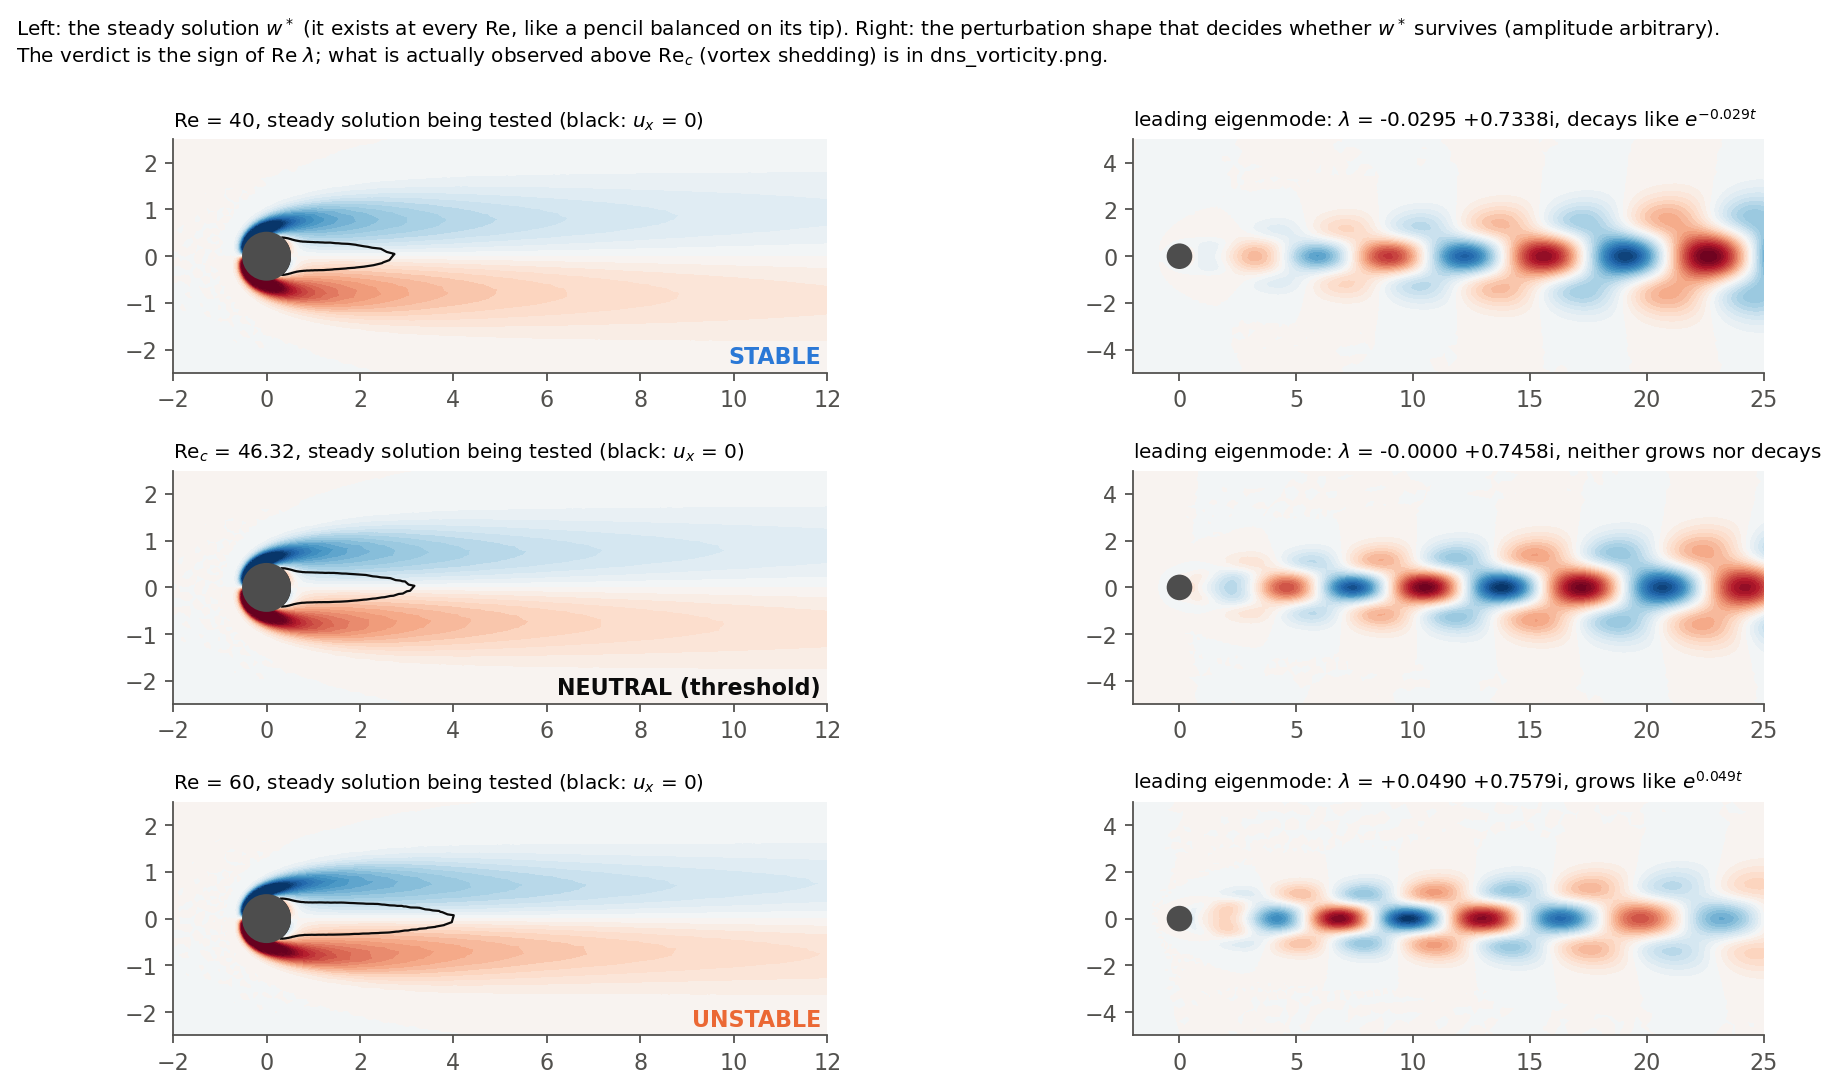
\includegraphics[width=\linewidth,height=182mm,keepaspectratio]{figures/wake_base_flow_and_eigenmode.png}\captionof{figure}[Archived figure]{Steady cylinder base flows and leading perturbations below, near, and above the Hopf threshold. The unstable symmetric steady solution is a valid base state even when nonlinear dynamics sheds vortices. \textit{Source:} \path{Ruben/Navier_Stokes_Inflow/stability/figures/base_flow_and_eigenmode.png}. First added 2026-09-29.}\end{center}
\clearpage
\begin{center}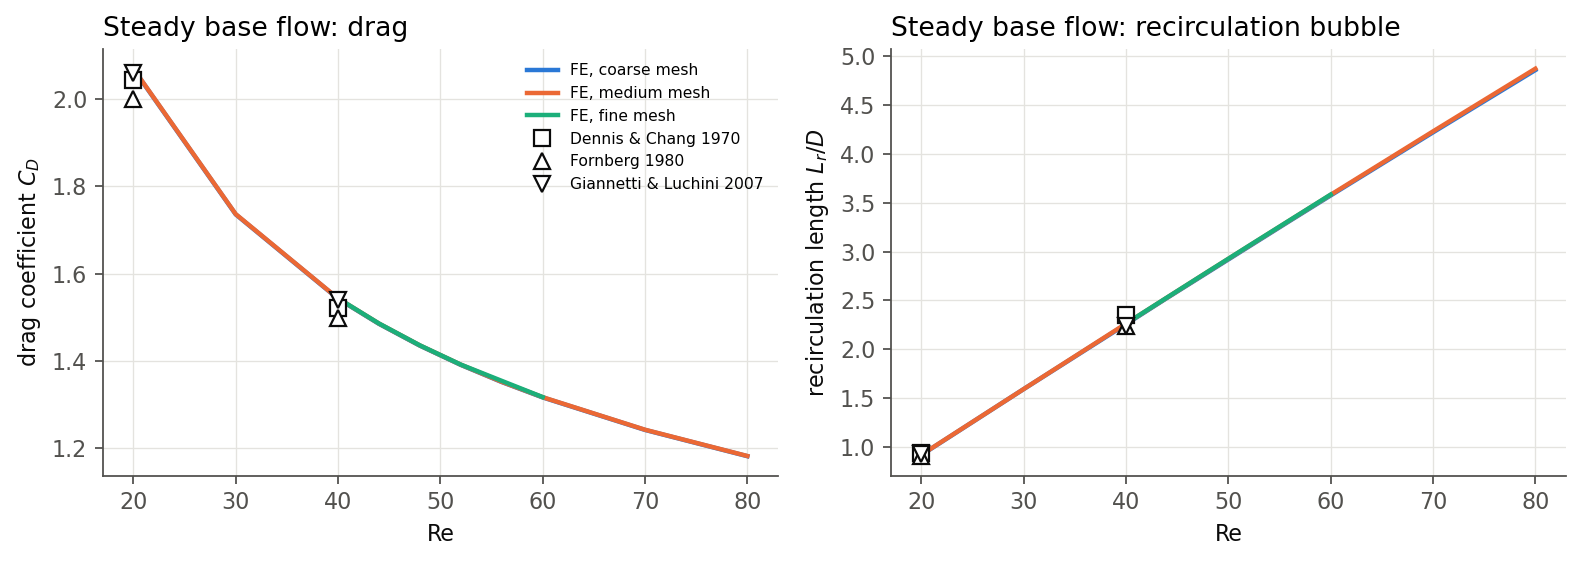
\includegraphics[width=\linewidth,height=86mm,keepaspectratio]{figures/wake_base_flow_validation.png}\captionof{figure}[Archived figure]{Cylinder drag and recirculation length compared with reference values. This tests the base solver independently of the eigensolver. \textit{Source:} \path{Ruben/Navier_Stokes_Inflow/stability/figures/base_flow_validation.png}. First added 2026-09-29.}\end{center}
\begin{center}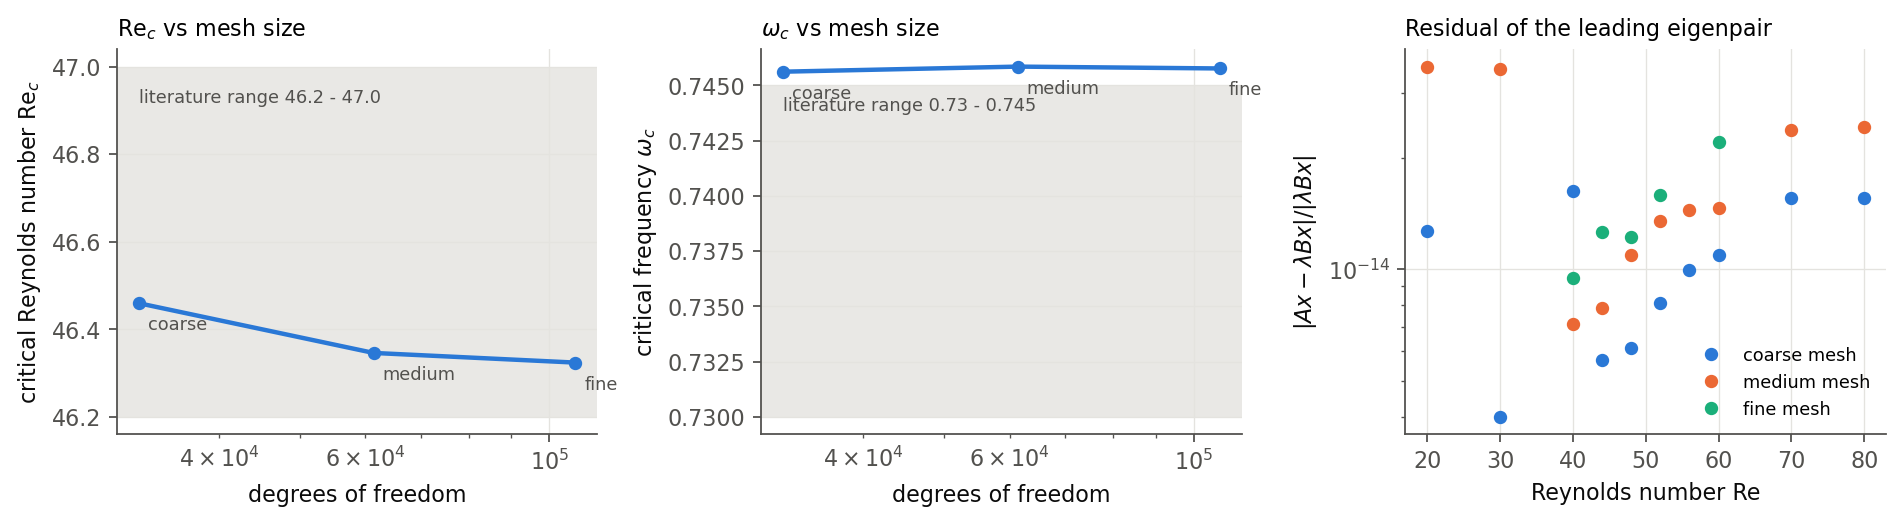
\includegraphics[width=\linewidth,height=86mm,keepaspectratio]{figures/wake_convergence_and_residuals.png}\captionof{figure}[Archived figure]{Cylinder onset, frequency, and eigenpair residuals under mesh refinement. The residual checks numerical solution of the discrete problem; mesh changes test its approximation to the continuum. \textit{Source:} \path{Ruben/Navier_Stokes_Inflow/stability/figures/convergence_and_residuals.png}. First added 2026-09-29.}\end{center}
\clearpage
\begin{center}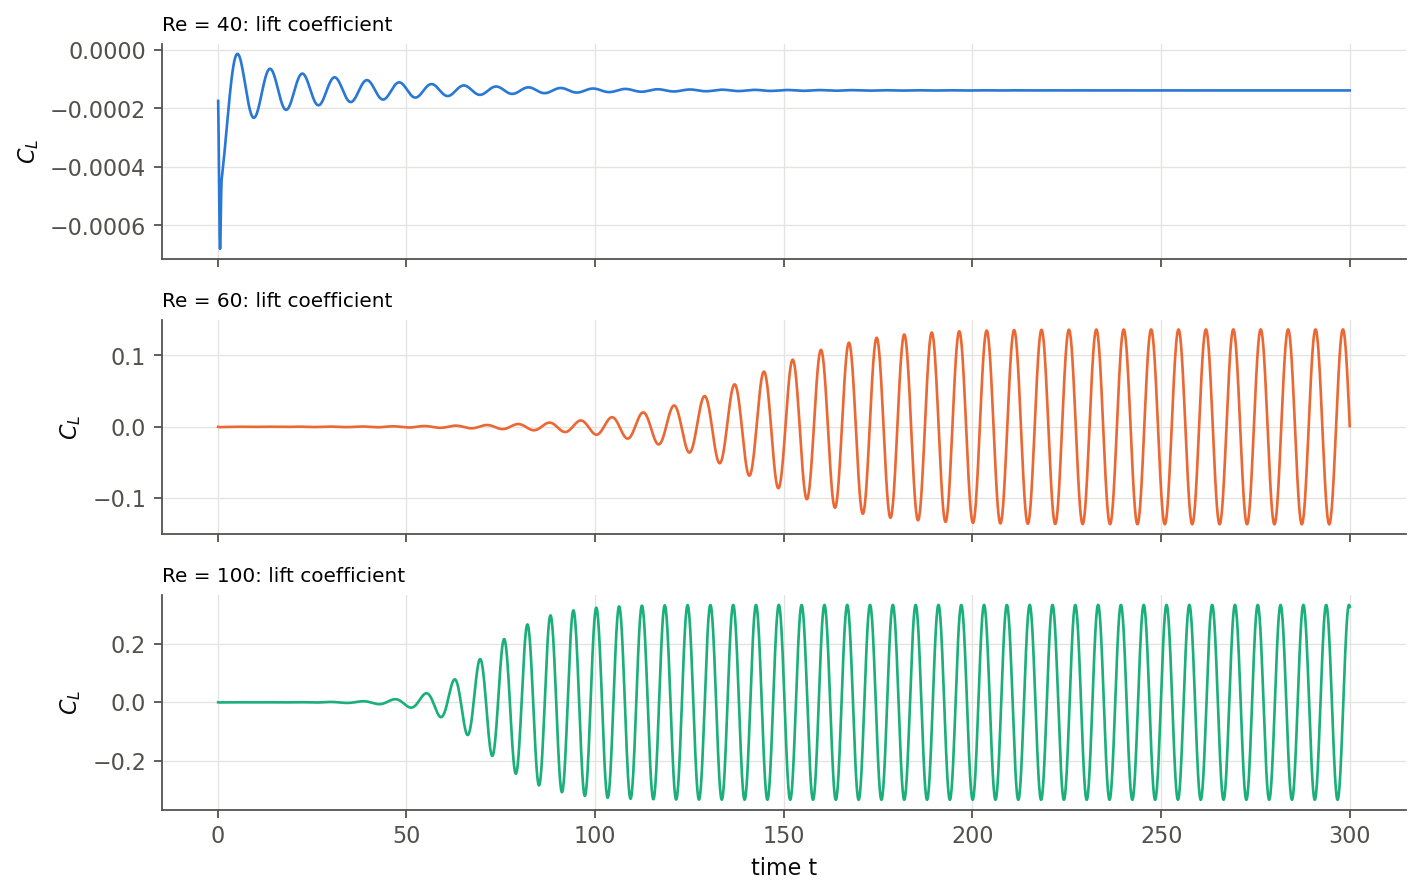
\includegraphics[width=\linewidth,height=182mm,keepaspectratio]{figures/wake_dns_lift.png}\captionof{figure}[Archived figure]{Lift time series at Reynolds numbers 40, 60, and 100. The low-Reynolds-number perturbation decays; the unstable cases grow and saturate in vortex shedding. \textit{Source:} \path{Ruben/Navier_Stokes_Inflow/stability/figures/dns_lift.png}. First added 2026-09-29.}\end{center}
\clearpage
\begin{center}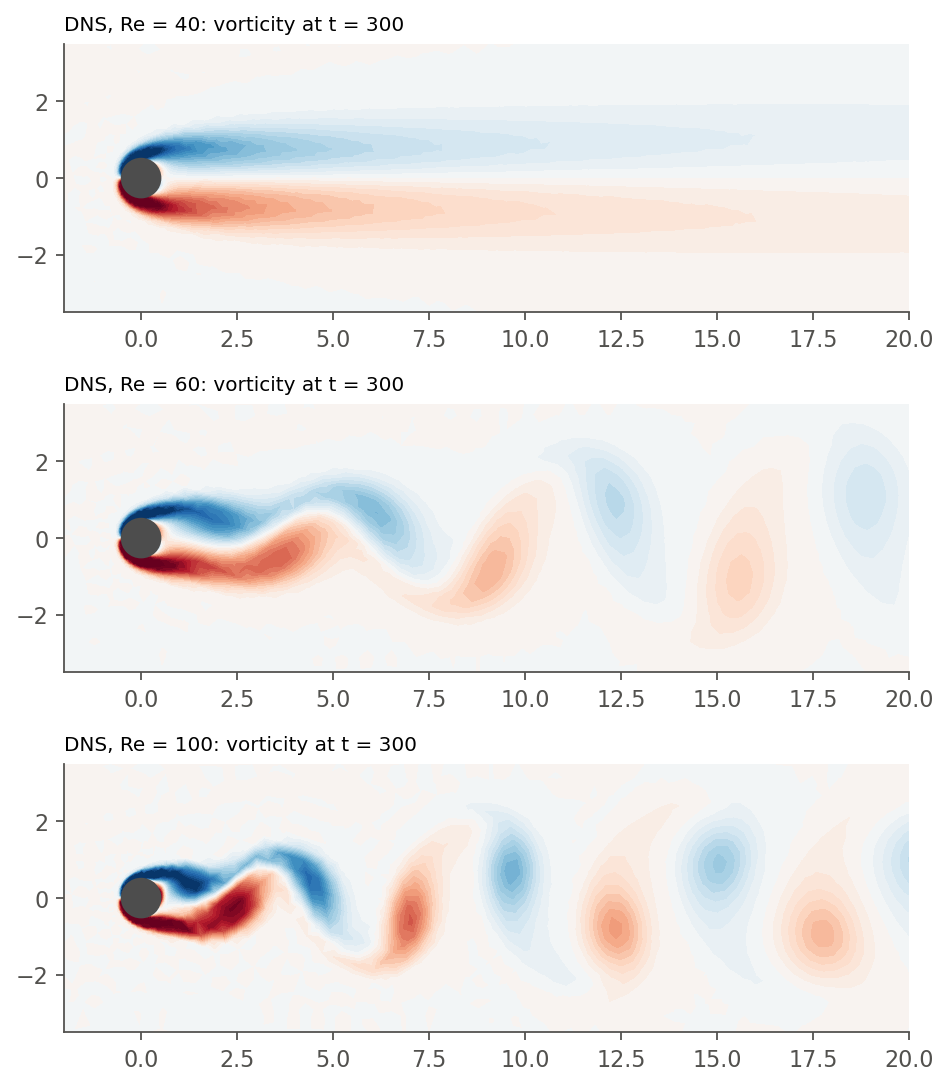
\includegraphics[width=\linewidth,height=182mm,keepaspectratio]{figures/wake_dns_vorticity.png}\captionof{figure}[Archived figure]{Nonlinear cylinder-wake snapshots for the benchmark runs. The vortex street above onset provides an independent dynamical check of the computed Hopf instability. \textit{Source:} \path{Ruben/Navier_Stokes_Inflow/stability/figures/dns_vorticity.png}. First added 2026-09-29.}\end{center}
\clearpage
\begin{center}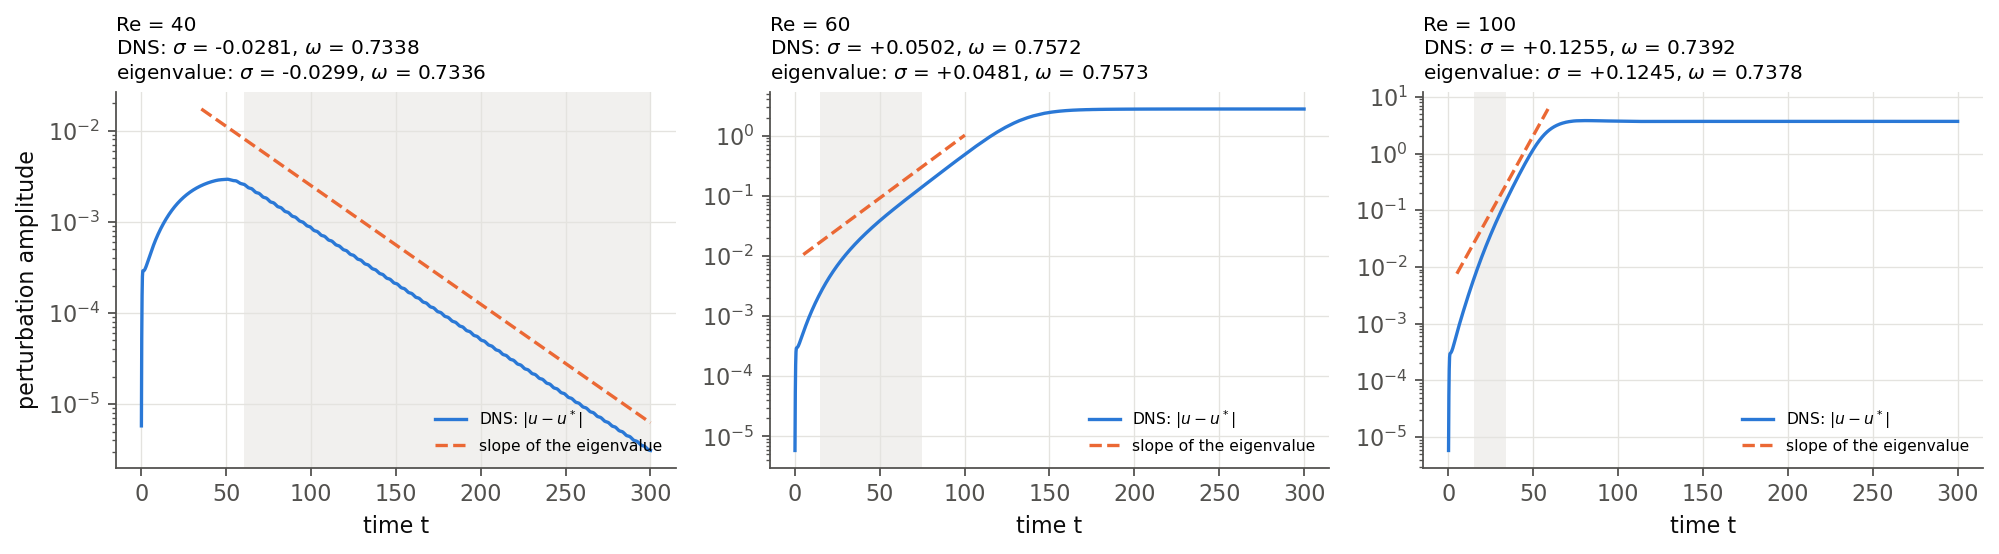
\includegraphics[width=\linewidth,height=182mm,keepaspectratio]{figures/wake_dns_vs_eigenvalues.png}\captionof{figure}[Archived figure]{Perturbation amplitude in cylinder DNS compared with exponential eigenvalue predictions. Growth is fitted in the linear interval before nonlinear saturation. \textit{Source:} \path{Ruben/Navier_Stokes_Inflow/stability/figures/dns_vs_eigenvalues.png}. First added 2026-09-29.}\end{center}
\clearpage
\begin{center}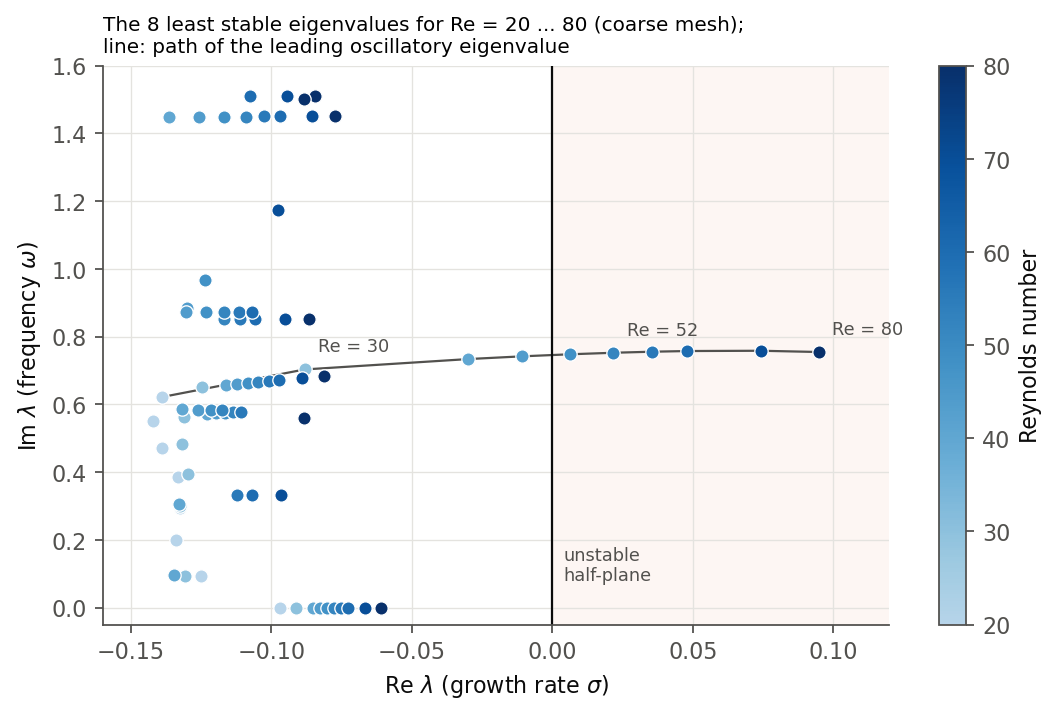
\includegraphics[width=\linewidth,height=182mm,keepaspectratio]{figures/wake_eigenvalue_trajectories.png}\captionof{figure}[Archived figure]{Cylinder eigenvalue trajectories as Reynolds number varies. The relevant oscillatory pair can be missed by searching only near the origin. \textit{Source:} \path{Ruben/Navier_Stokes_Inflow/stability/figures/eigenvalue_trajectories.png}. First added 2026-09-29.}\end{center}
\clearpage
\begin{center}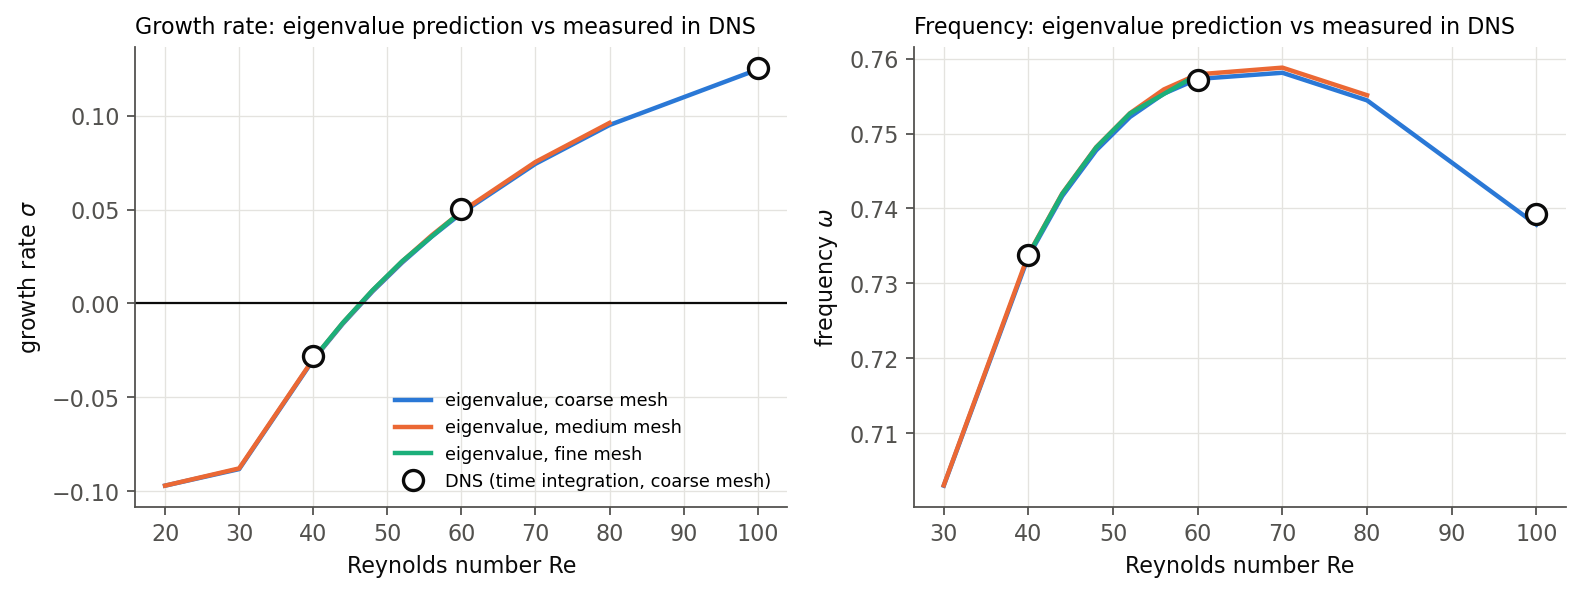
\includegraphics[width=\linewidth,height=86mm,keepaspectratio]{figures/wake_eigenvalues_vs_dns.png}\captionof{figure}[Archived figure]{Cylinder growth rates and frequencies from eigenanalysis and nonlinear time integration. Agreement is strongest for frequency and within a few percent for the fitted growth rates. \textit{Source:} \path{Ruben/Navier_Stokes_Inflow/stability/figures/eigenvalues_vs_dns.png}. First added 2026-09-29.}\end{center}
\begin{center}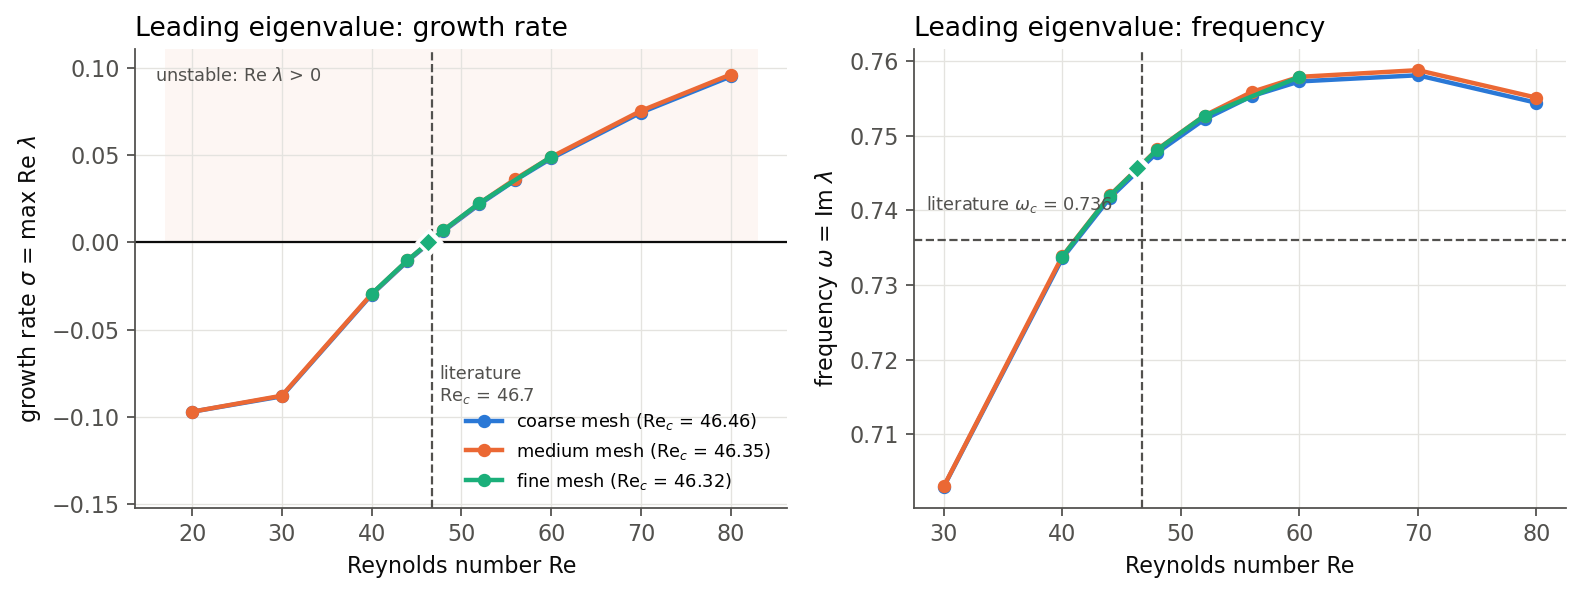
\includegraphics[width=\linewidth,height=86mm,keepaspectratio]{figures/wake_growth_rate_vs_Re.png}\captionof{figure}[Archived figure]{Leading cylinder growth rate and frequency versus Reynolds number on three meshes. The first instability occurs near Reynolds number 46.3. \textit{Source:} \path{Ruben/Navier_Stokes_Inflow/stability/figures/growth_rate_vs_Re.png}. First added 2026-09-29.}\end{center}
\clearpage
\begin{center}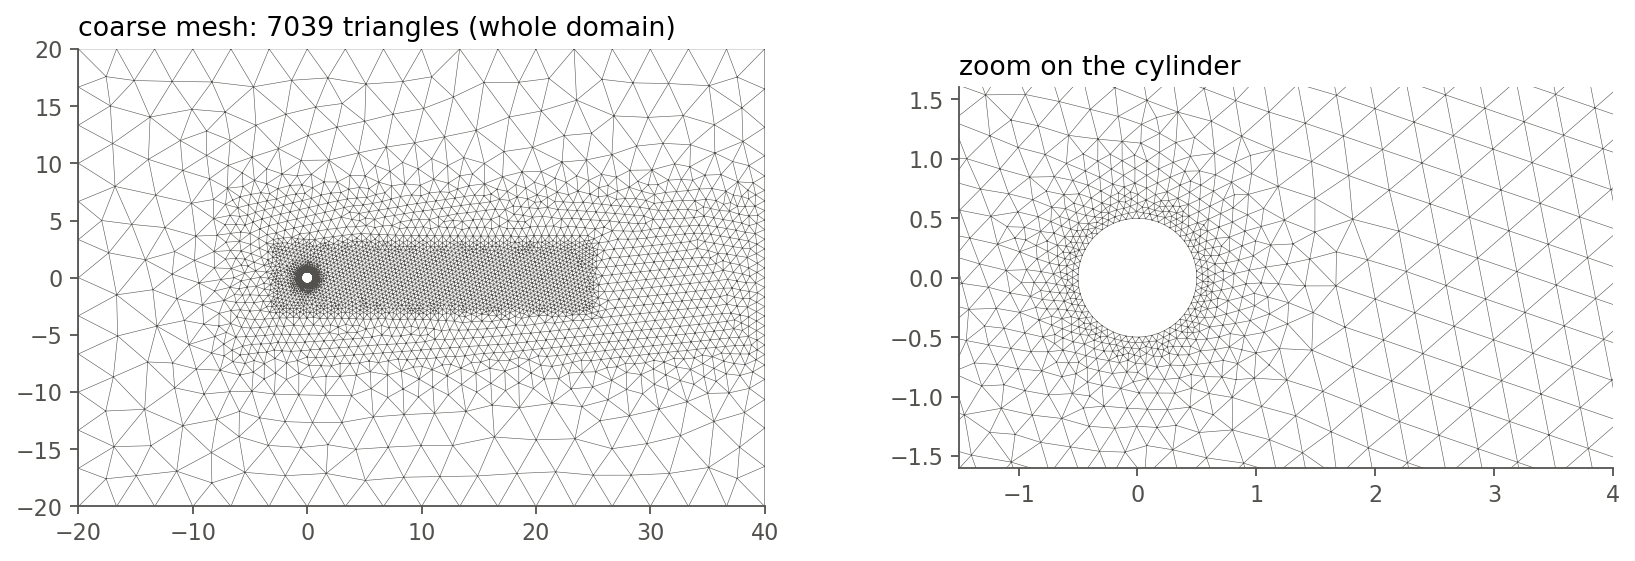
\includegraphics[width=\linewidth,height=86mm,keepaspectratio]{figures/wake_mesh_coarse.png}\captionof{figure}[Archived figure]{Coarse cylinder mesh, including a close view of the obstacle. This is the first of the three benchmark resolutions. \textit{Source:} \path{Ruben/Navier_Stokes_Inflow/stability/figures/mesh_coarse.png}. First added 2026-09-29.}\end{center}
\begin{center}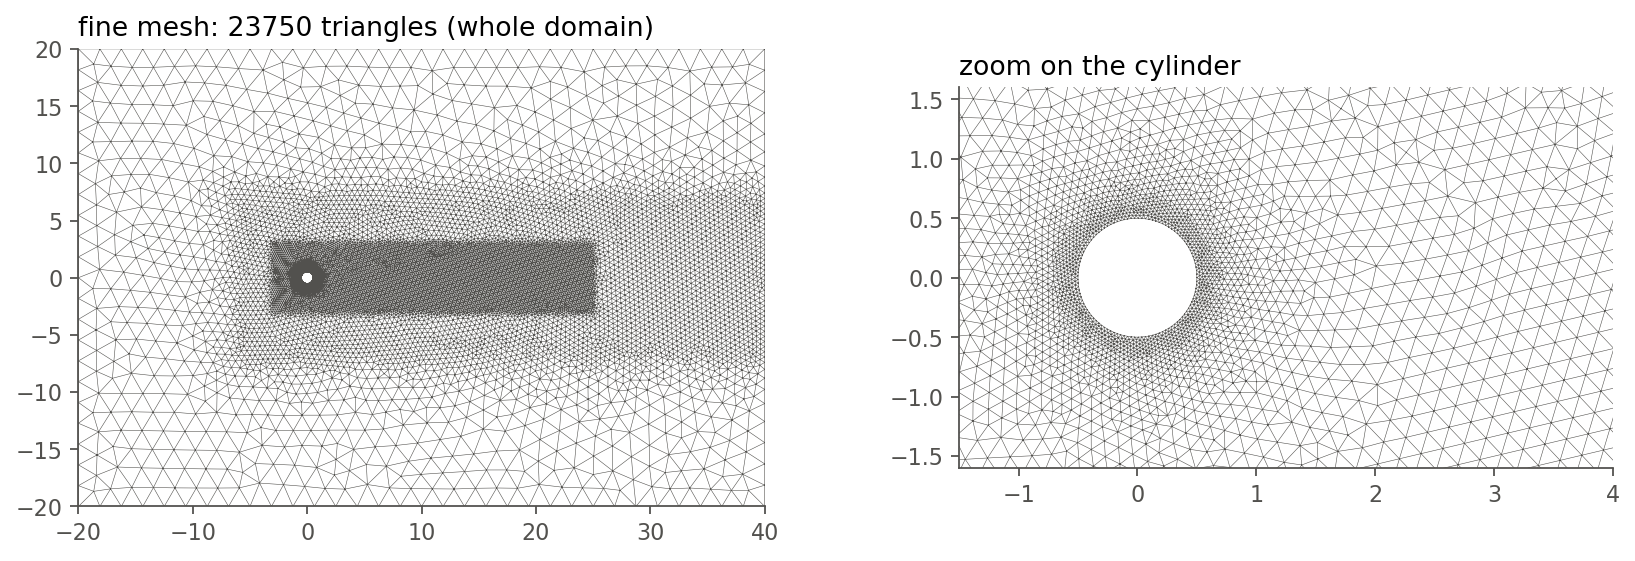
\includegraphics[width=\linewidth,height=86mm,keepaspectratio]{figures/wake_mesh_fine.png}\captionof{figure}[Archived figure]{Fine cylinder mesh and obstacle refinement. It gives the reported benchmark onset near Reynolds number 46.32. \textit{Source:} \path{Ruben/Navier_Stokes_Inflow/stability/figures/mesh_fine.png}. First added 2026-09-29.}\end{center}
\clearpage
\begin{center}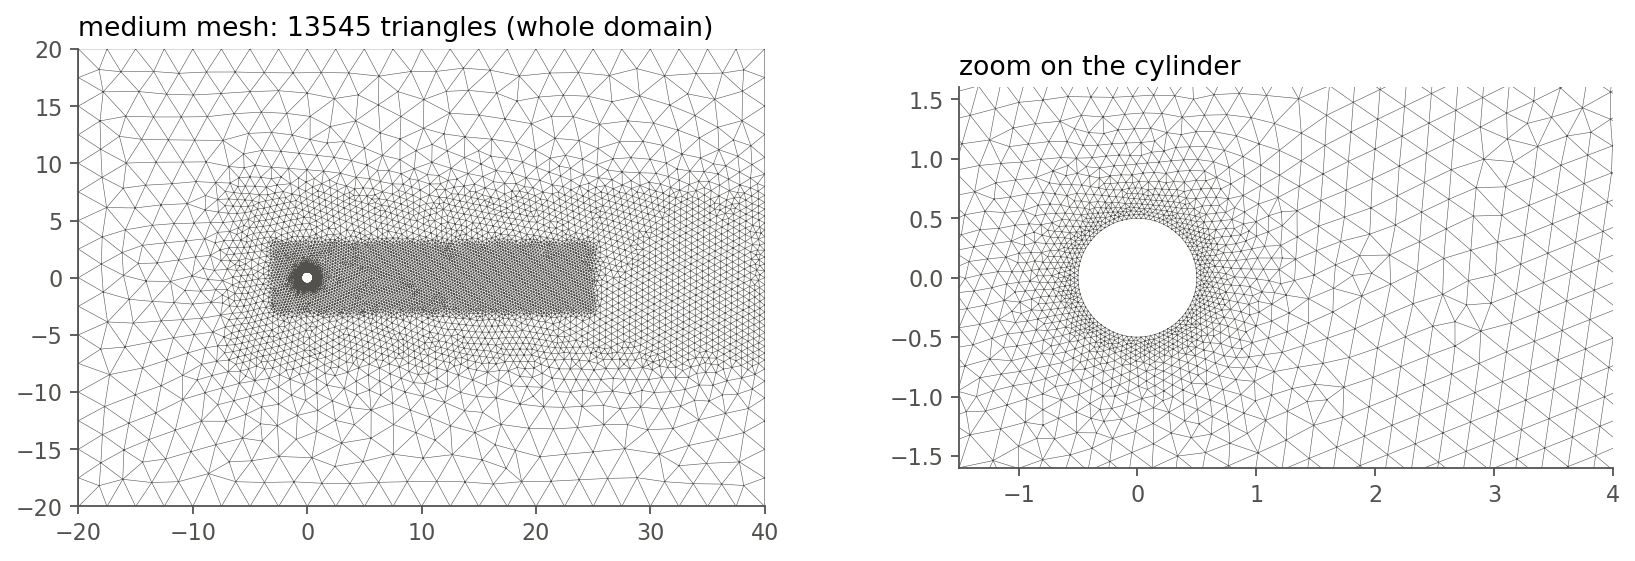
\includegraphics[width=\linewidth,height=86mm,keepaspectratio]{figures/wake_mesh_medium.png}\captionof{figure}[Archived figure]{Intermediate cylinder mesh and obstacle refinement. It supplies the middle point of the convergence sequence. \textit{Source:} \path{Ruben/Navier_Stokes_Inflow/stability/figures/mesh_medium.png}. First added 2026-09-29.}\end{center}
\begin{center}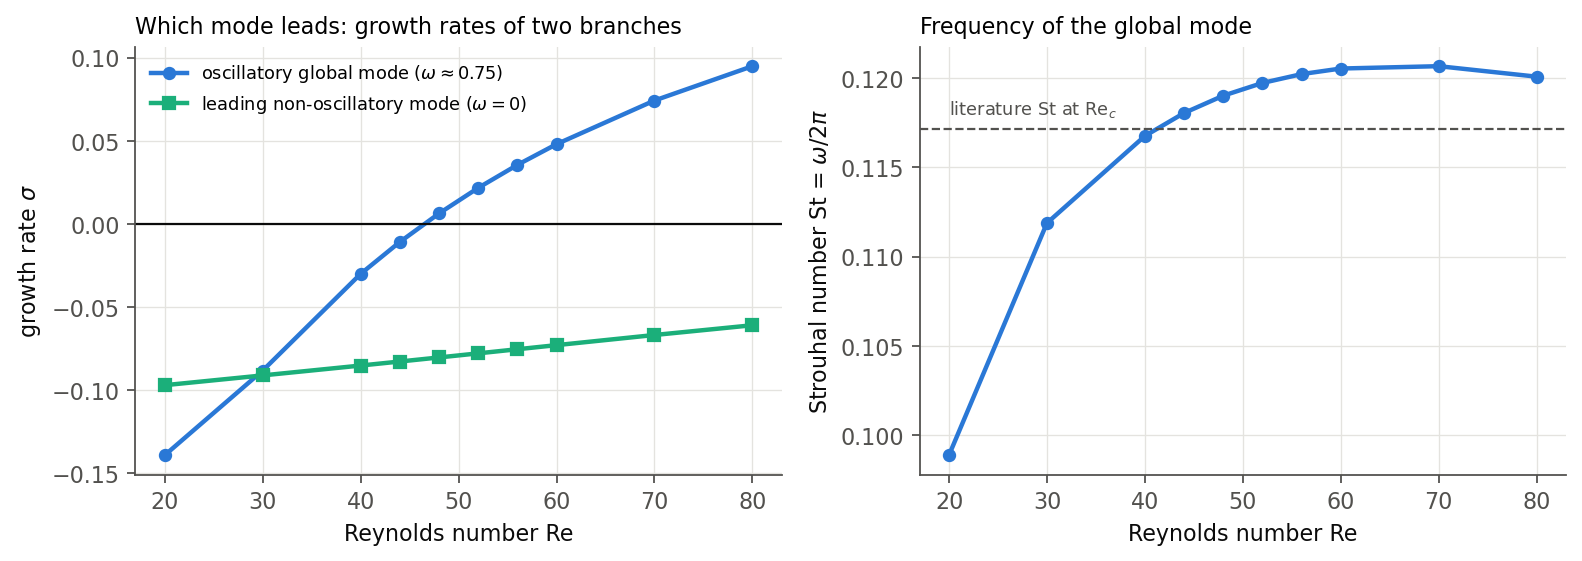
\includegraphics[width=\linewidth,height=86mm,keepaspectratio]{figures/wake_mode_branches_vs_Re.png}\captionof{figure}[Archived figure]{Competing cylinder growth-rate branches and the leading Hopf Strouhal number. Selecting the least damped returned eigenpair requires covering the relevant complex-frequency range. \textit{Source:} \path{Ruben/Navier_Stokes_Inflow/stability/figures/mode_branches_vs_Re.png}. First added 2026-09-29.}\end{center}
\clearpage
\begin{center}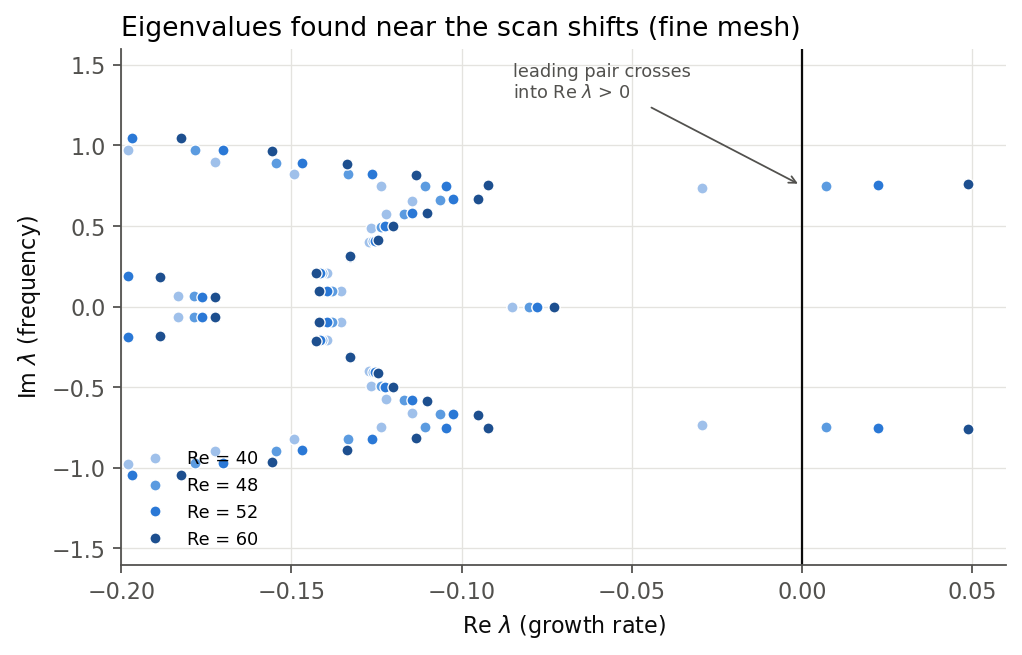
\includegraphics[width=\linewidth,height=182mm,keepaspectratio]{figures/wake_spectra.png}\captionof{figure}[Archived figure]{Cylinder spectra near the sampled complex shifts. The Hopf pair and dense damped cluster illustrate why a real shift alone is insufficient. \textit{Source:} \path{Ruben/Navier_Stokes_Inflow/stability/figures/spectra.png}. First added 2026-09-29.}\end{center}
\clearpage
\begin{center}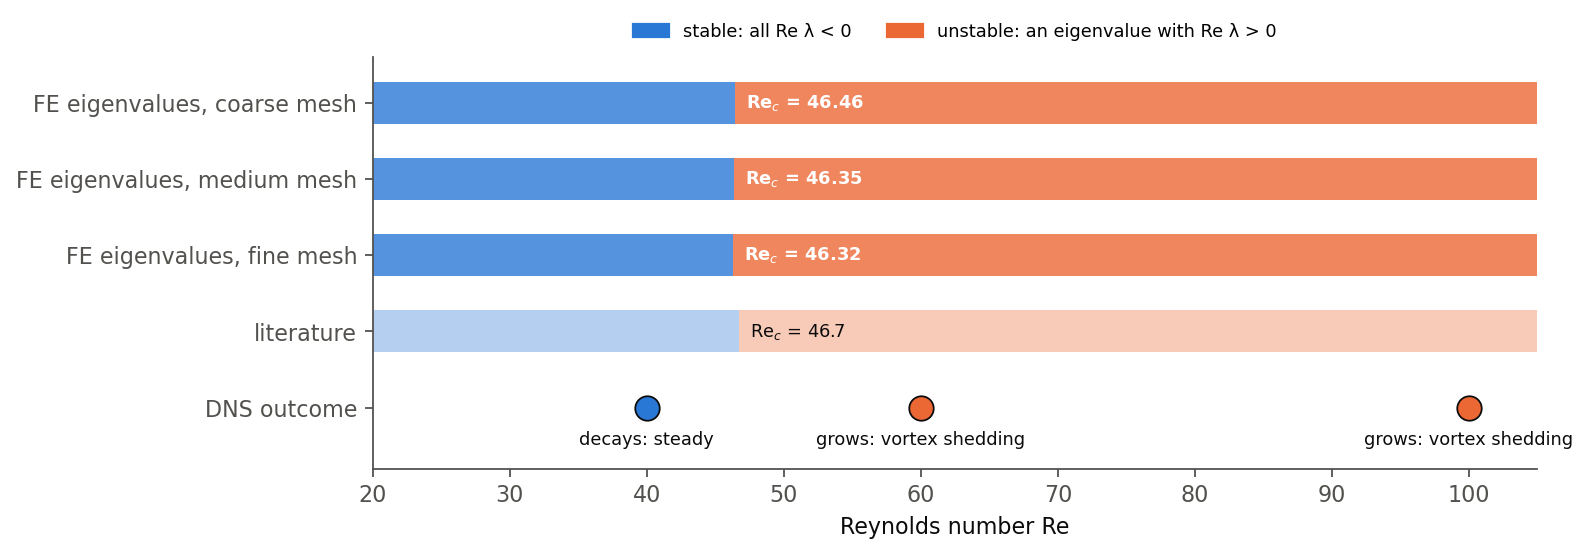
\includegraphics[width=\linewidth,height=86mm,keepaspectratio]{figures/wake_stability_map.png}\captionof{figure}[Archived figure]{Cylinder stable/unstable classification from eigenvalues and independent DNS outcomes. Threshold differences across meshes are small but remain measurable. \textit{Source:} \path{Ruben/Navier_Stokes_Inflow/stability/figures/stability_map.png}. First added 2026-09-29.}\end{center}
\begin{center}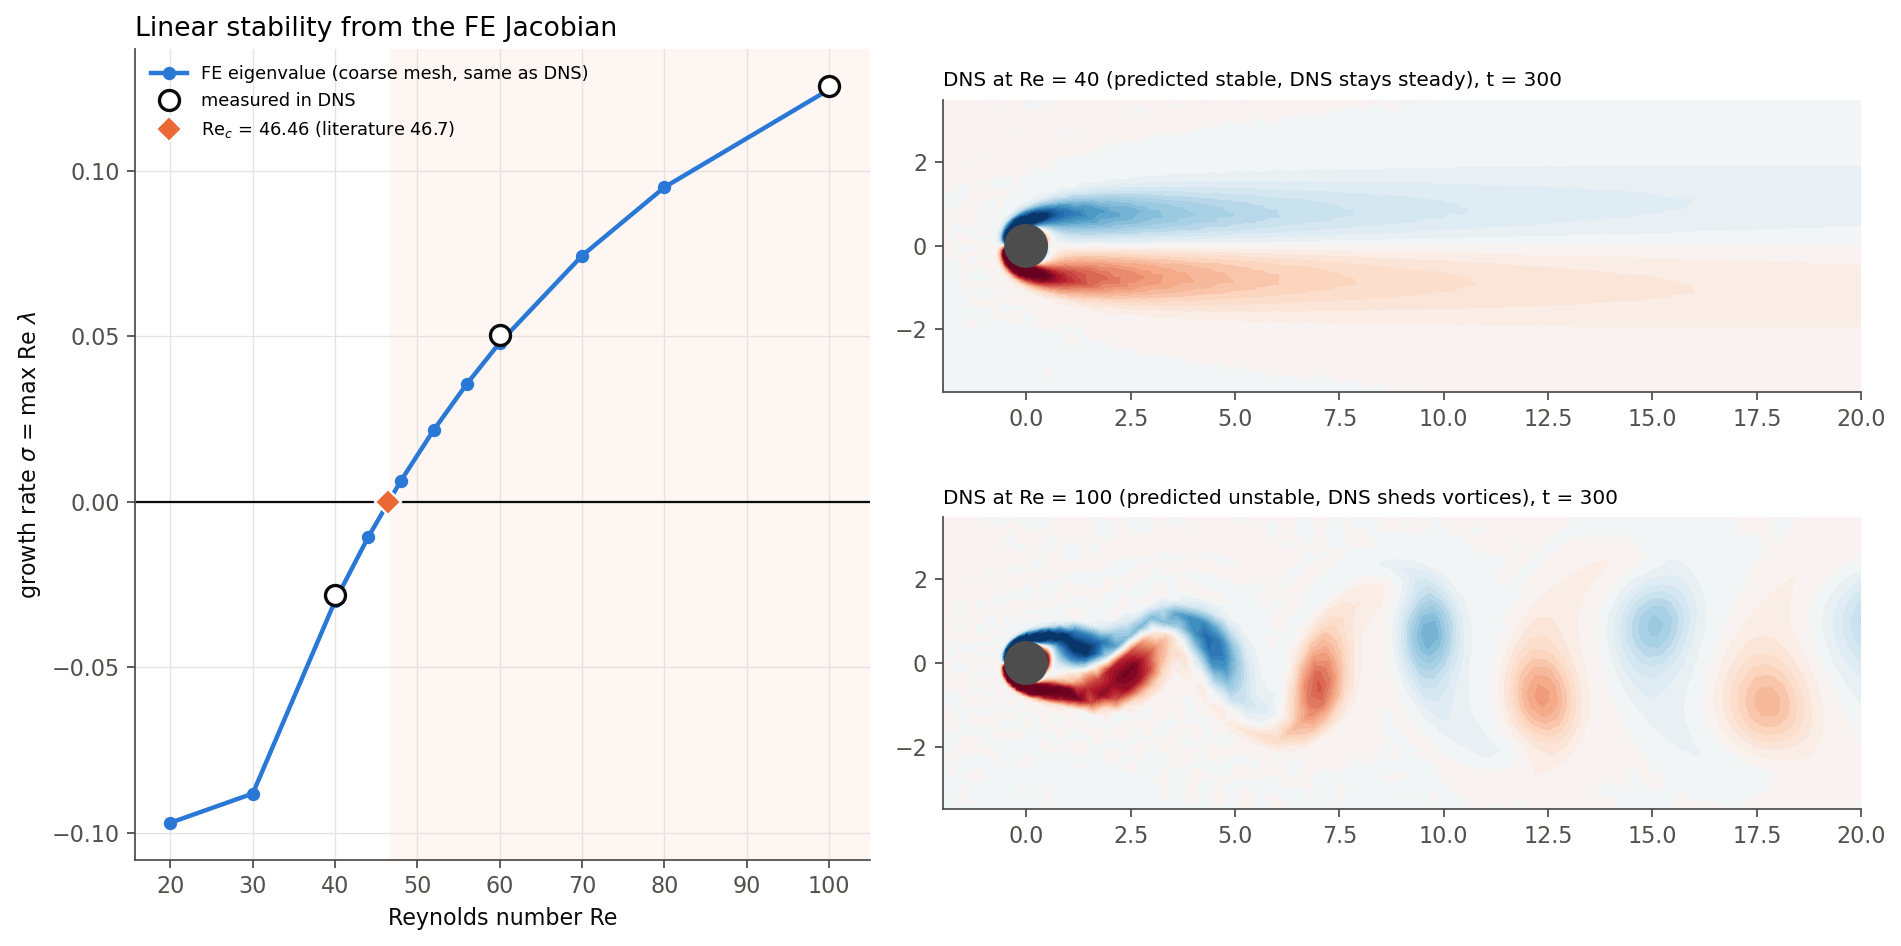
\includegraphics[width=\linewidth,height=86mm,keepaspectratio]{figures/wake_summary.png}\captionof{figure}[Archived figure]{Overview of the cylinder benchmark: leading growth rate, threshold, and contrasting nonlinear outcomes below and above onset. \textit{Source:} \path{Ruben/Navier_Stokes_Inflow/stability/figures/summary.png}. First added 2026-09-29.}\end{center}
\clearpage
\begin{center}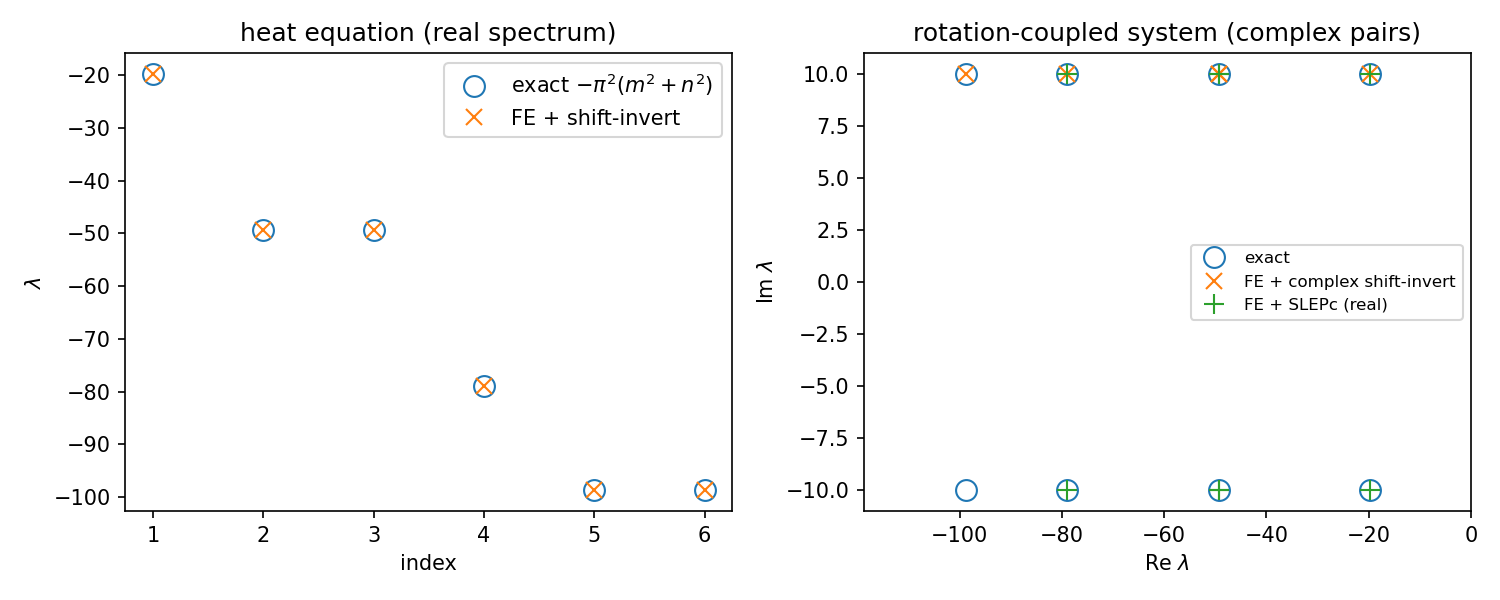
\includegraphics[width=\linewidth,height=182mm,keepaspectratio]{figures/wake_check_eigensolver.png}\captionof{figure}[Archived figure]{Generic eigensolver checks on a heat equation and a rotation-coupled system with complex eigenpairs. Both real and complex spectral calculations are tested against exact values. \textit{Source:} \path{Ruben/Navier_Stokes_Inflow/stability/solution/checks/check_eigensolver.png}. First added 2026-09-29.}\end{center}
\clearpage
\begin{center}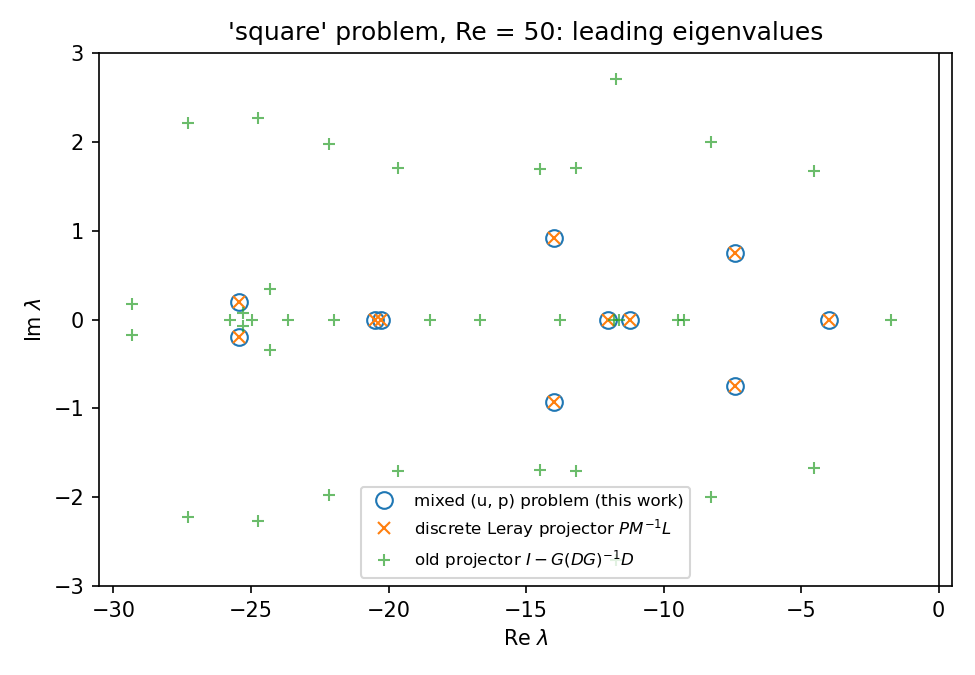
\includegraphics[width=\linewidth,height=182mm,keepaspectratio]{figures/wake_check_projector_equivalence.png}\captionof{figure}[Archived figure]{Mixed incompressible eigenproblem compared with the correct discrete Leray projector. A Euclidean projector is a different operator and produces different spectra. \textit{Source:} \path{Ruben/Navier_Stokes_Inflow/stability/solution/checks/check_projector_equivalence.png}. First added 2026-09-29.}\end{center}
\clearpage
\begin{center}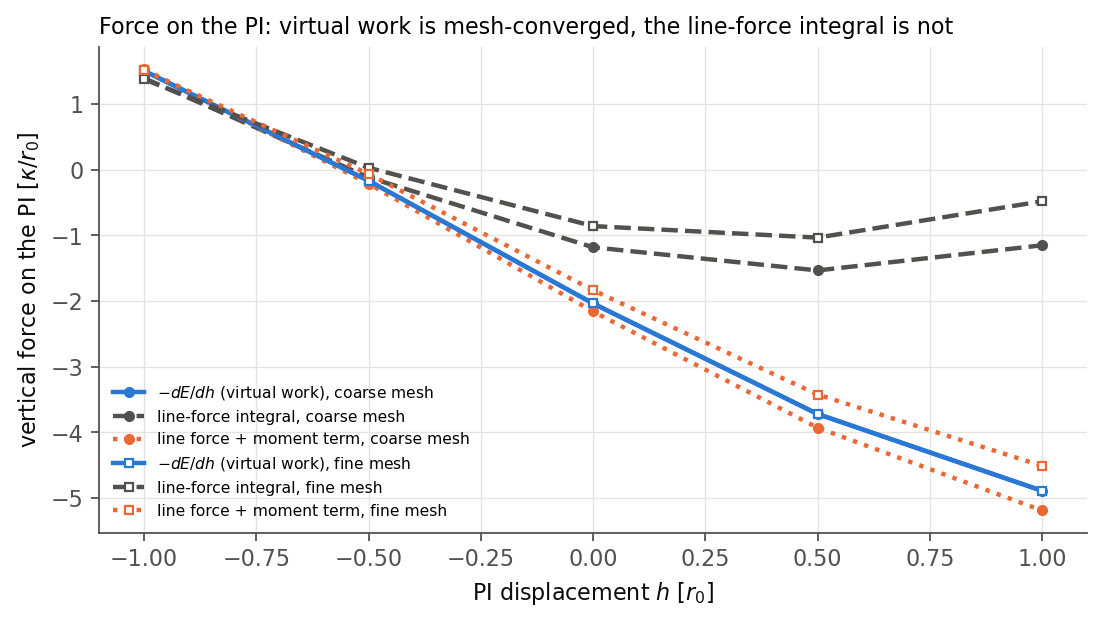
\includegraphics[width=\linewidth,height=182mm,keepaspectratio]{figures/membrane_check_force_methods.png}\captionof{figure}[Archived figure]{Ring force diagnostic under refinement. Virtual work converges; the original boundary line integral does not. Adding the moment term improves a coarse result but does not remove the boundary-derivative discretization error. \textit{Source:} \path{Ruben/membrane_stability/figures/check_force_methods.png}. First added 2026-09-29.}\end{center}
\clearpage
\begin{center}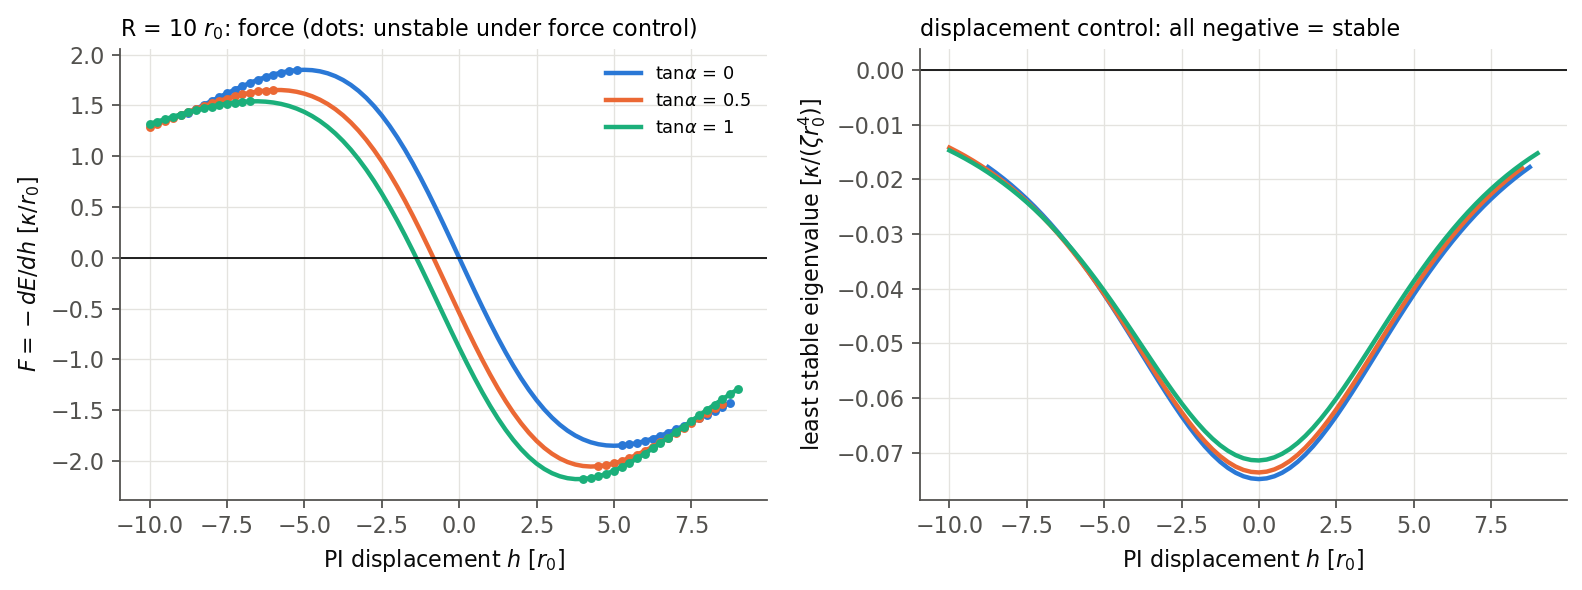
\includegraphics[width=\linewidth,height=86mm,keepaspectratio]{figures/membrane_contact_angle_R10.png}\captionof{figure}[Archived figure]{Contact-slope dependence of ring force and leading relaxation rate at outer radius ten. Force extrema shift, while the sampled height-controlled branches remain stable. \textit{Source:} \path{Ruben/membrane_stability/figures/contact_angle_R10.png}. First added 2026-09-29.}\end{center}
\begin{center}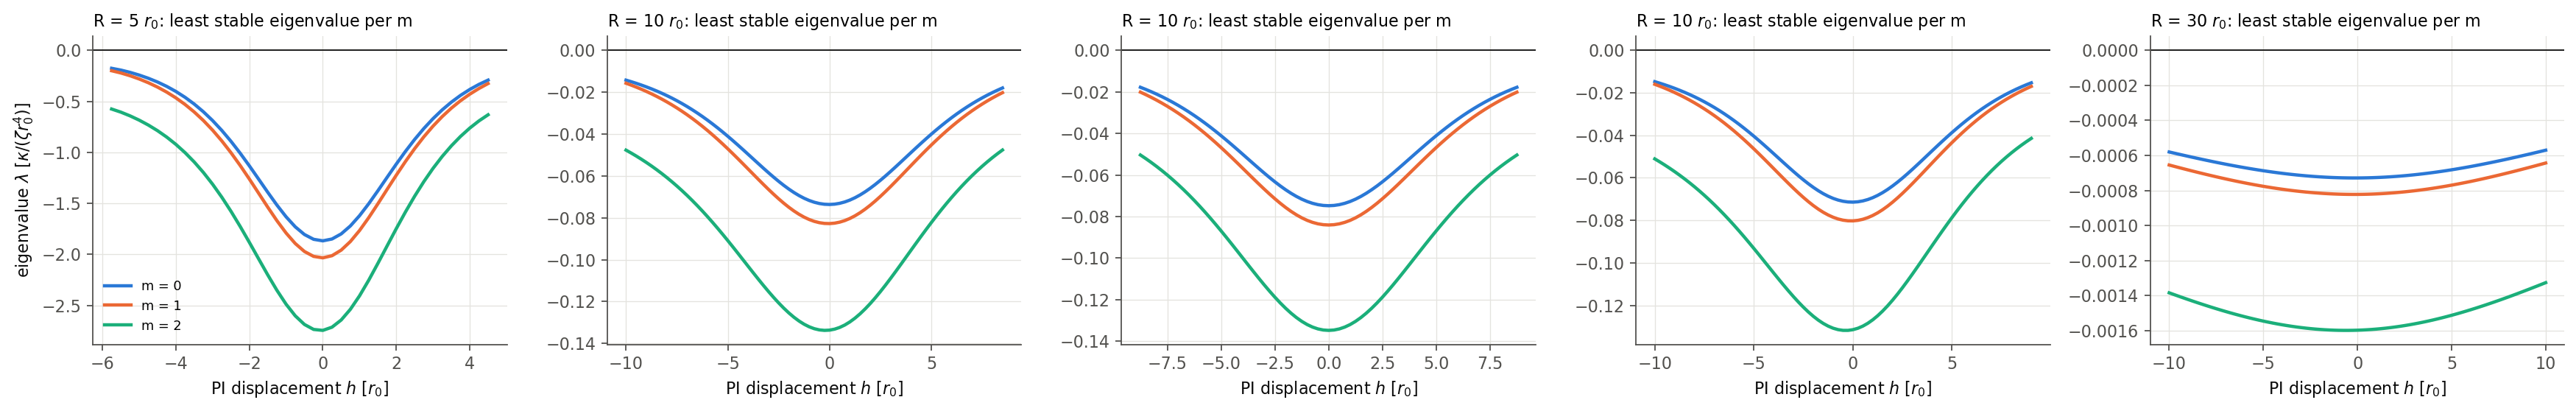
\includegraphics[width=\linewidth,height=86mm,keepaspectratio]{figures/membrane_eigenvalues_vs_h.png}\captionof{figure}[Archived figure]{Ring relaxation spectra versus protein height, resolved by azimuthal number. No growing fixed-height mode is found in these sampled branches; spectra soften as the neck becomes steep. \textit{Source:} \path{Ruben/membrane_stability/figures/eigenvalues_vs_h.png}. First added 2026-09-29.}\end{center}
\clearpage
\begin{center}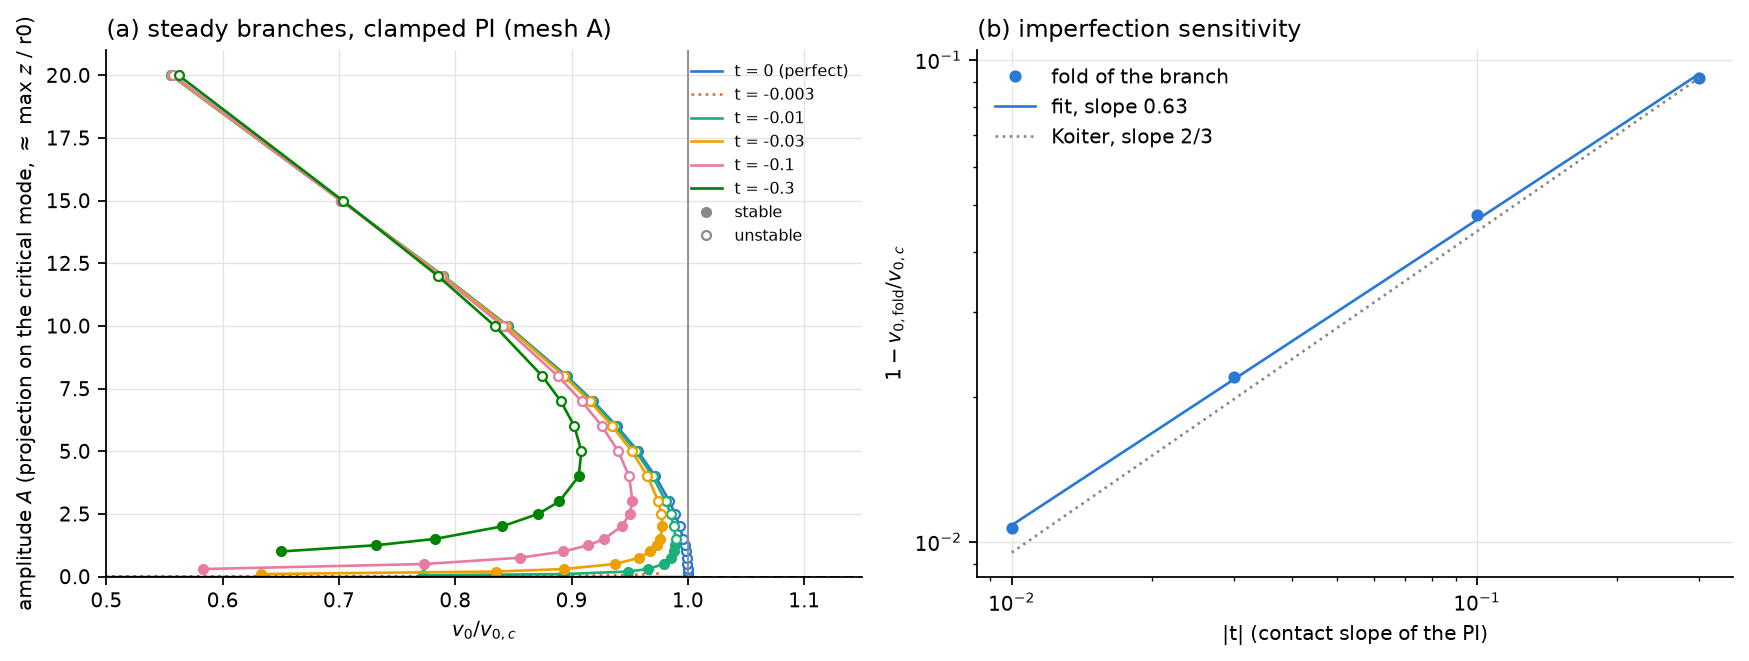
\includegraphics[width=\linewidth,height=86mm,keepaspectratio]{figures/membrane_flow2_bifurcation.png}\captionof{figure}[Archived figure]{Corrected clamped-protein continuation. The perfect branch is subcritical and a nonzero contact slope produces a fold; the fitted imperfection exponent is close to two thirds. The later projected theory supplies an independently computed prefactor. \textit{Source:} \path{Ruben/membrane_stability/figures/flow2_bifurcation.png}. First added 2026-09-30.}\end{center}
\begin{center}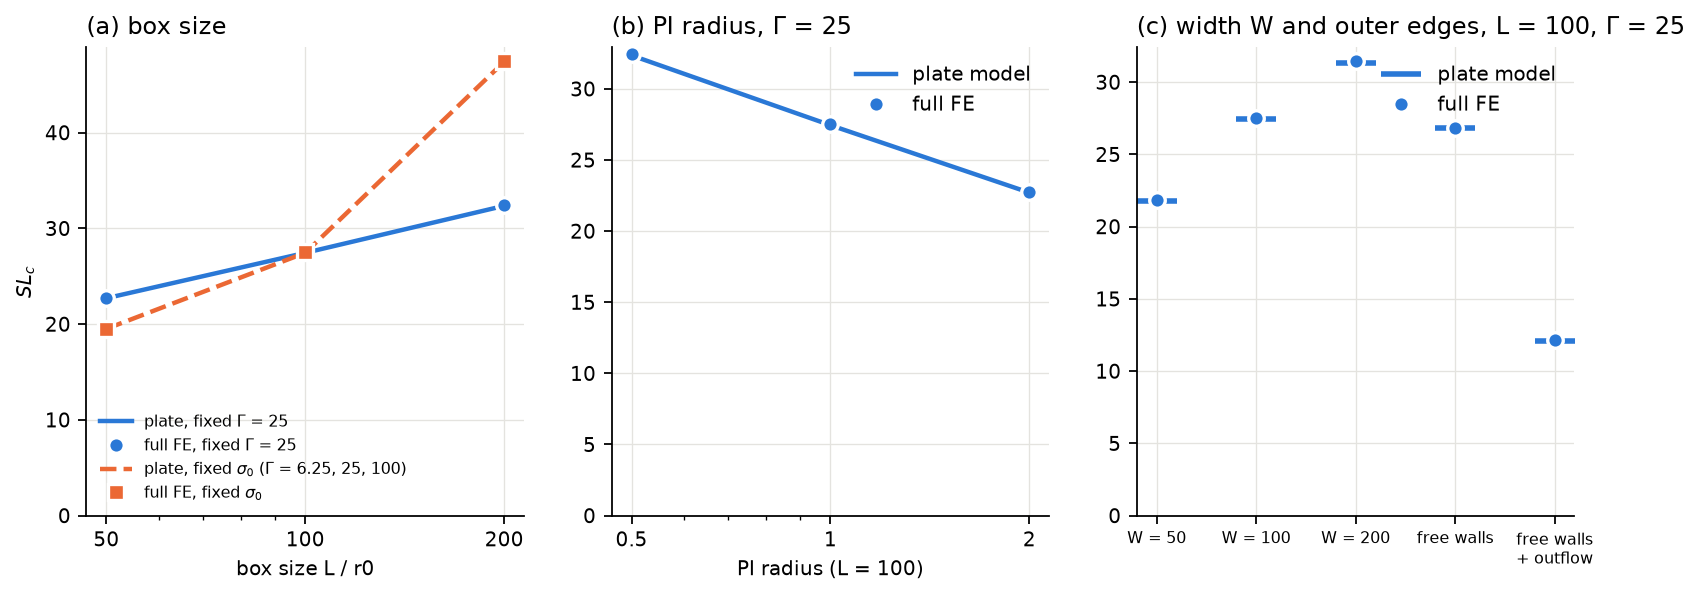
\includegraphics[width=\linewidth,height=86mm,keepaspectratio]{figures/membrane_flow2_domain.png}\captionof{figure}[Archived figure]{Corrected physical thresholds versus domain length, protein radius, width, and outer-height constraints. Fixed-tension and fixed-Gamma size sweeps are different experiments. \textit{Source:} \path{Ruben/membrane_stability/figures/flow2_domain.png}. First added 2026-09-30.}\end{center}
\clearpage
\begin{center}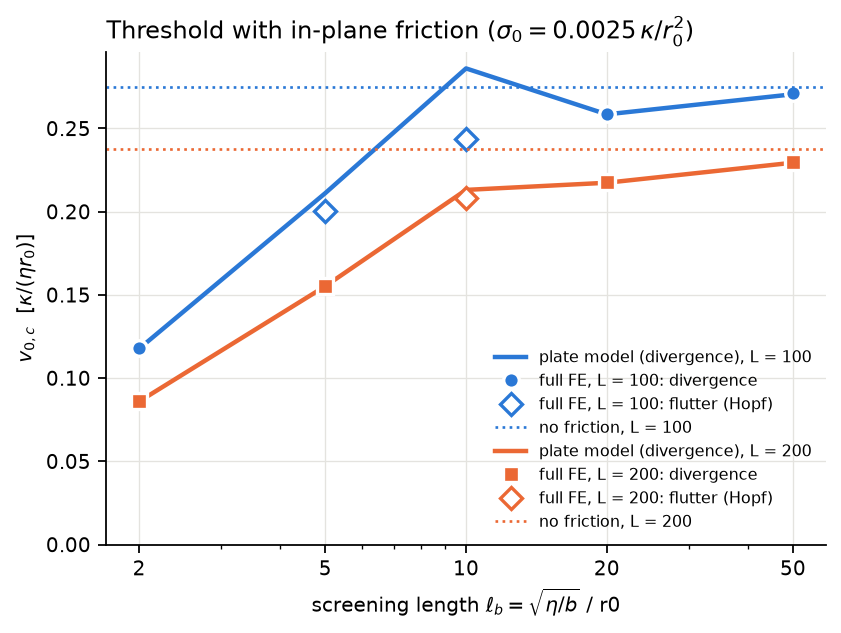
\includegraphics[width=\linewidth,height=182mm,keepaspectratio]{figures/membrane_flow2_friction.png}\captionof{figure}[Archived figure]{Early friction comparison showing divergence thresholds and full-equation flutter crossings. The real plate threshold curve alone is not the first onset when a complex pair crosses earlier; the later map in the archive resolves this. \textit{Source:} \path{Ruben/membrane_stability/figures/flow2_friction.png}. First added 2026-09-30.}\end{center}
\clearpage
\begin{center}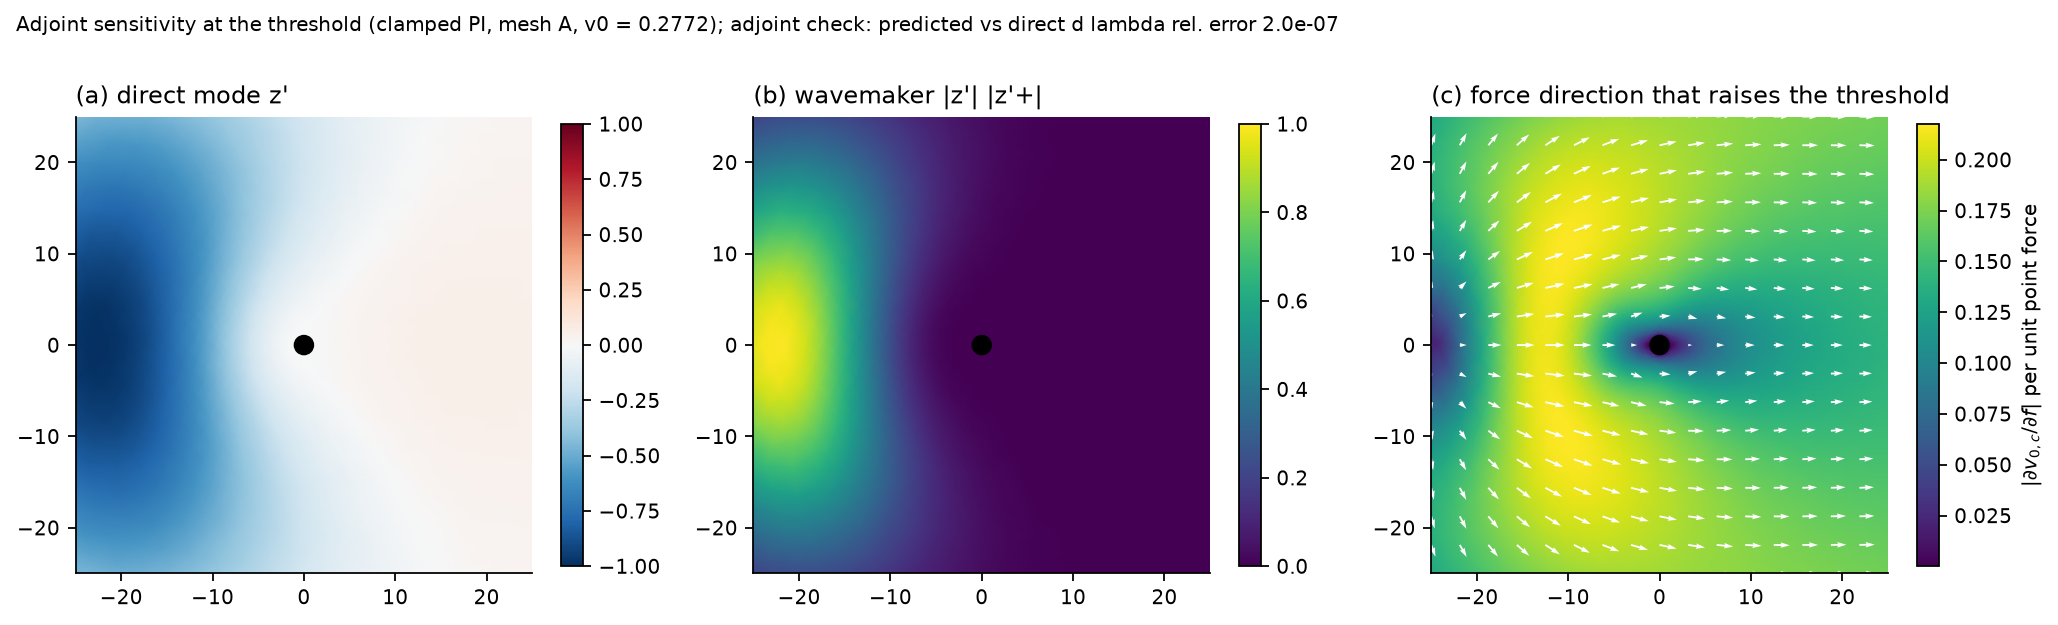
\includegraphics[width=\linewidth,height=86mm,keepaspectratio]{figures/membrane_flow2_sensitivity.png}\captionof{figure}[Archived figure]{Normal direct/adjoint shape, wavemaker, and tangential-force direction that increases the reference threshold. The strong response is located upstream of the inclusion. \textit{Source:} \path{Ruben/membrane_stability/figures/flow2_sensitivity.png}. First added 2026-09-30.}\end{center}
\begin{center}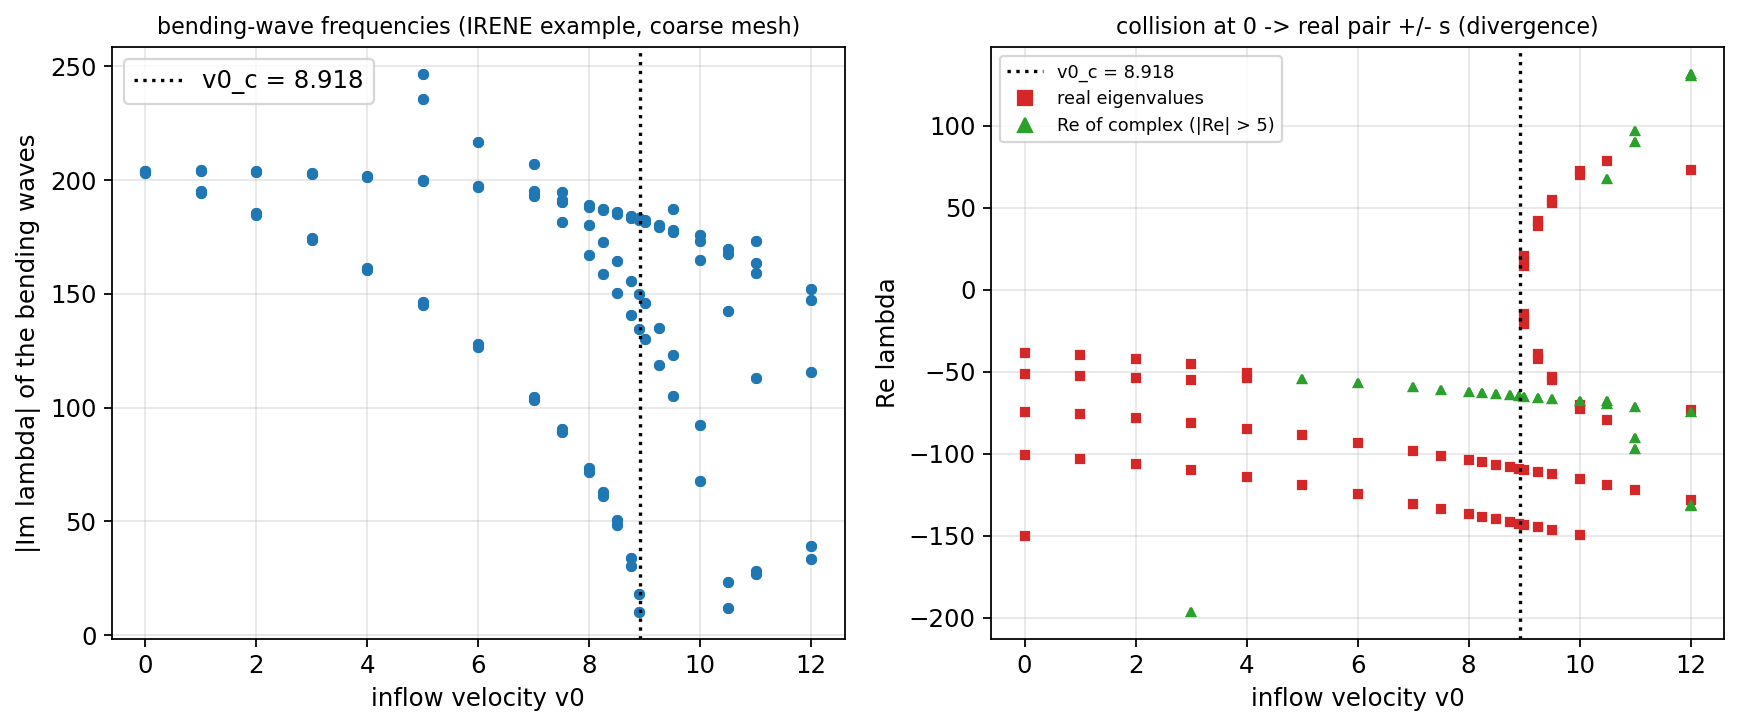
\includegraphics[width=\linewidth,height=86mm,keepaspectratio]{figures/membrane_flow_irene_example_collision.png}\captionof{figure}[Archived figure]{Inertial bending-wave collision in the slip-inclusion example. This is an illustrative high-inertia mechanism, not the overdamped lipid-membrane threshold. \textit{Source:} \path{Ruben/membrane_stability/figures/flow_irene_example_collision.png}. First added 2026-09-30.}\end{center}
\clearpage
\begin{center}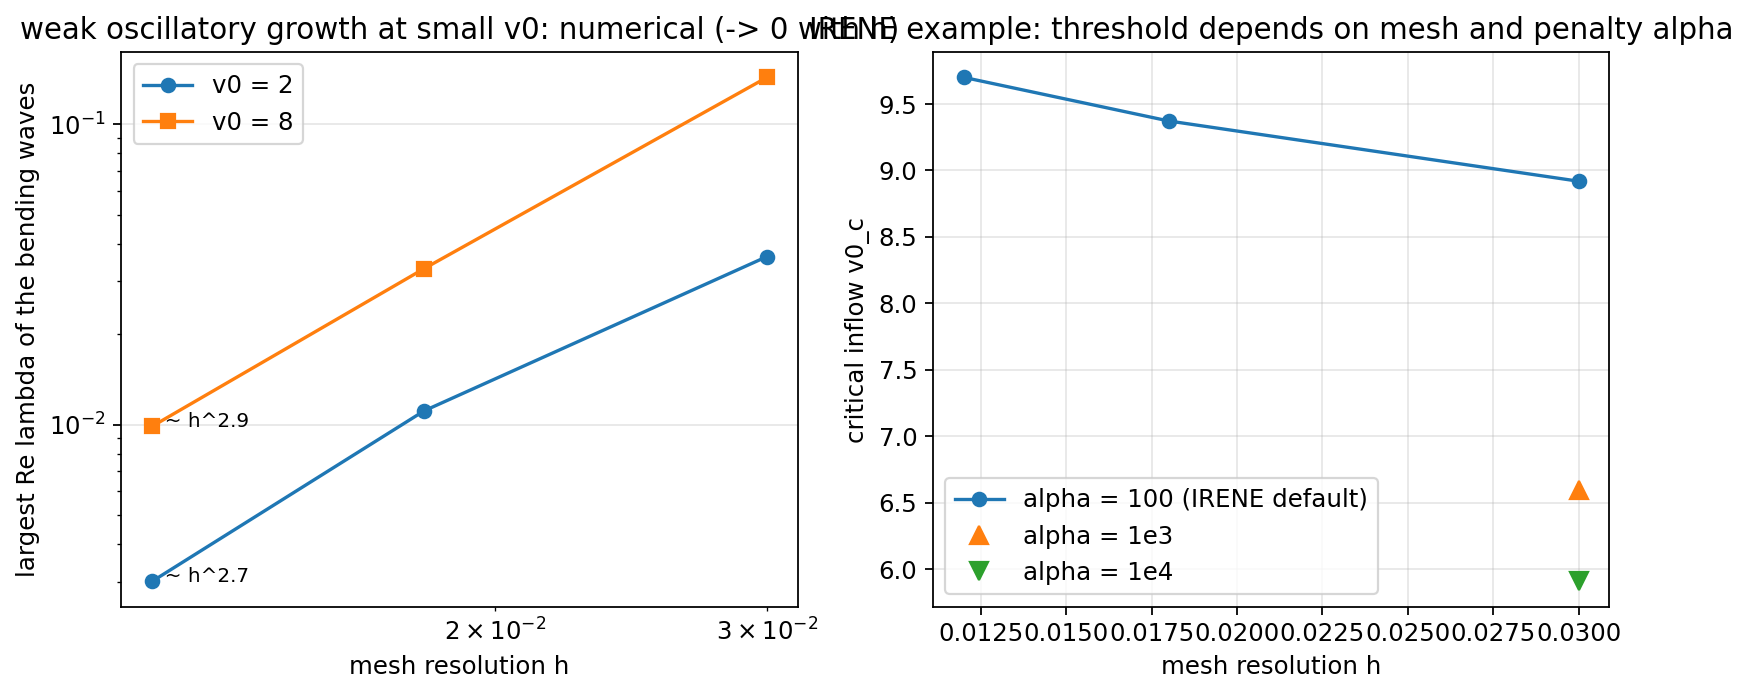
\includegraphics[width=\linewidth,height=182mm,keepaspectratio]{figures/membrane_flow_irene_example_convergence.png}\captionof{figure}[Archived figure]{Slip-penalty example: weak oscillatory growth shrinks with mesh size, while the apparent threshold depends strongly on penalty strength. These results diagnose numerical and boundary-condition sensitivity and are excluded from quantitative core claims. \textit{Source:} \path{Ruben/membrane_stability/figures/flow_irene_example_convergence.png}. First added 2026-09-30.}\end{center}
\clearpage
\begin{center}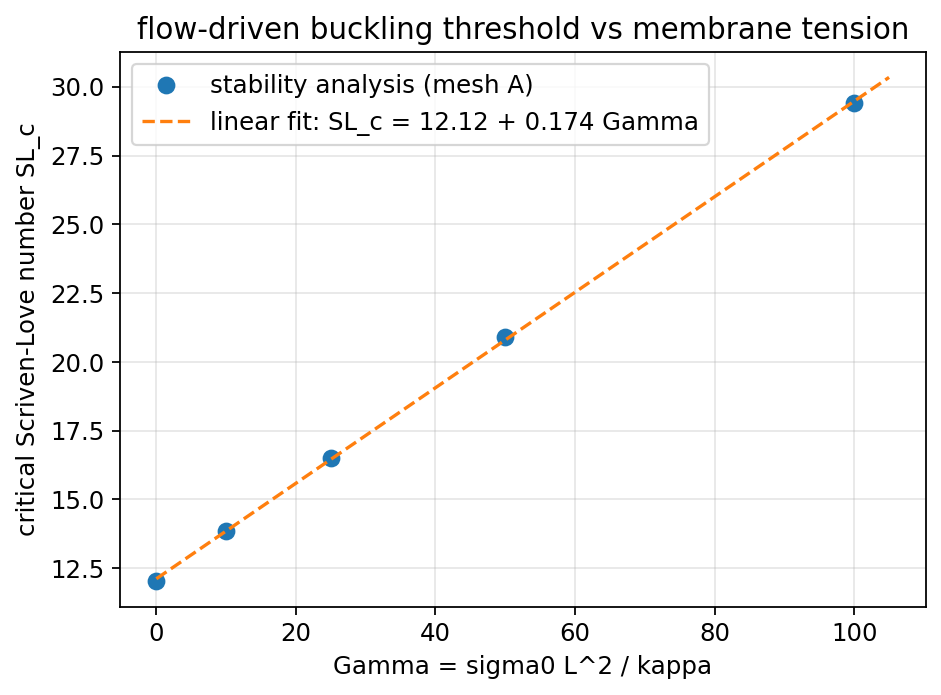
\includegraphics[width=\linewidth,height=182mm,keepaspectratio]{figures/membrane_flow_pre_SLc_vs_tension.png}\captionof{figure}[Archived figure]{Superseded original-rim calculation. Its approximate linear threshold-versus-tension fit belongs to the implementation without vertical protein force balance and must not be used for the corrected physical model. \textit{Source:} \path{Ruben/membrane_stability/figures/flow_pre_SLc_vs_tension.png}. First added 2026-09-30.}\end{center}
\clearpage
\begin{center}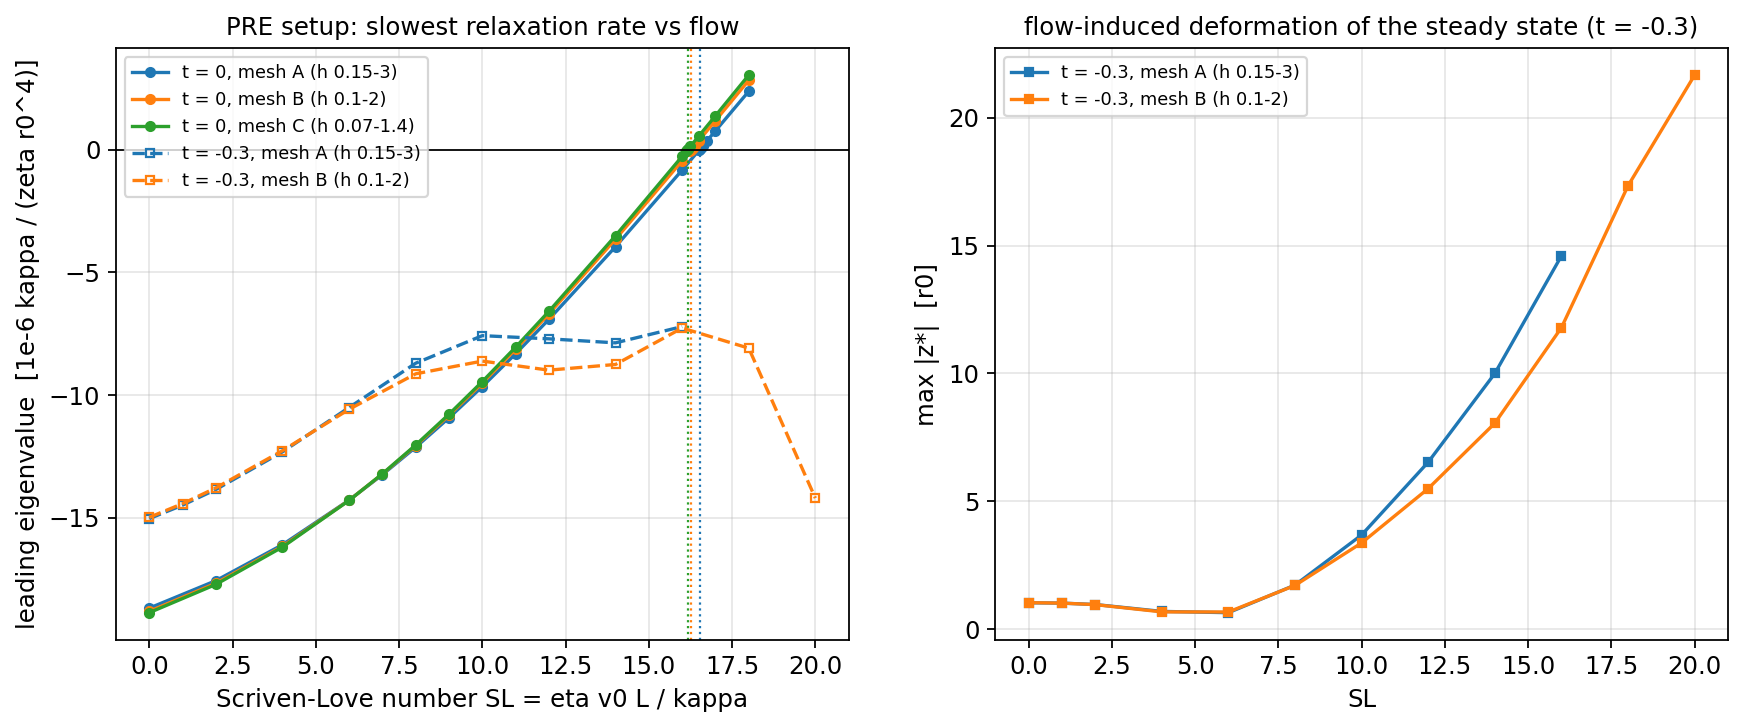
\includegraphics[width=\linewidth,height=86mm,keepaspectratio]{figures/membrane_flow_pre_eigenvalue_vs_SL.png}\captionof{figure}[Archived figure]{Superseded original-rim flow spectra and large imperfect deformation. The roughly sixteen threshold is a diagnostic of the original boundary-value problem; corrected thresholds are near twenty-seven in the reference geometry. \textit{Source:} \path{Ruben/membrane_stability/figures/flow_pre_eigenvalue_vs_SL.png}. First added 2026-09-30.}\end{center}
\begin{center}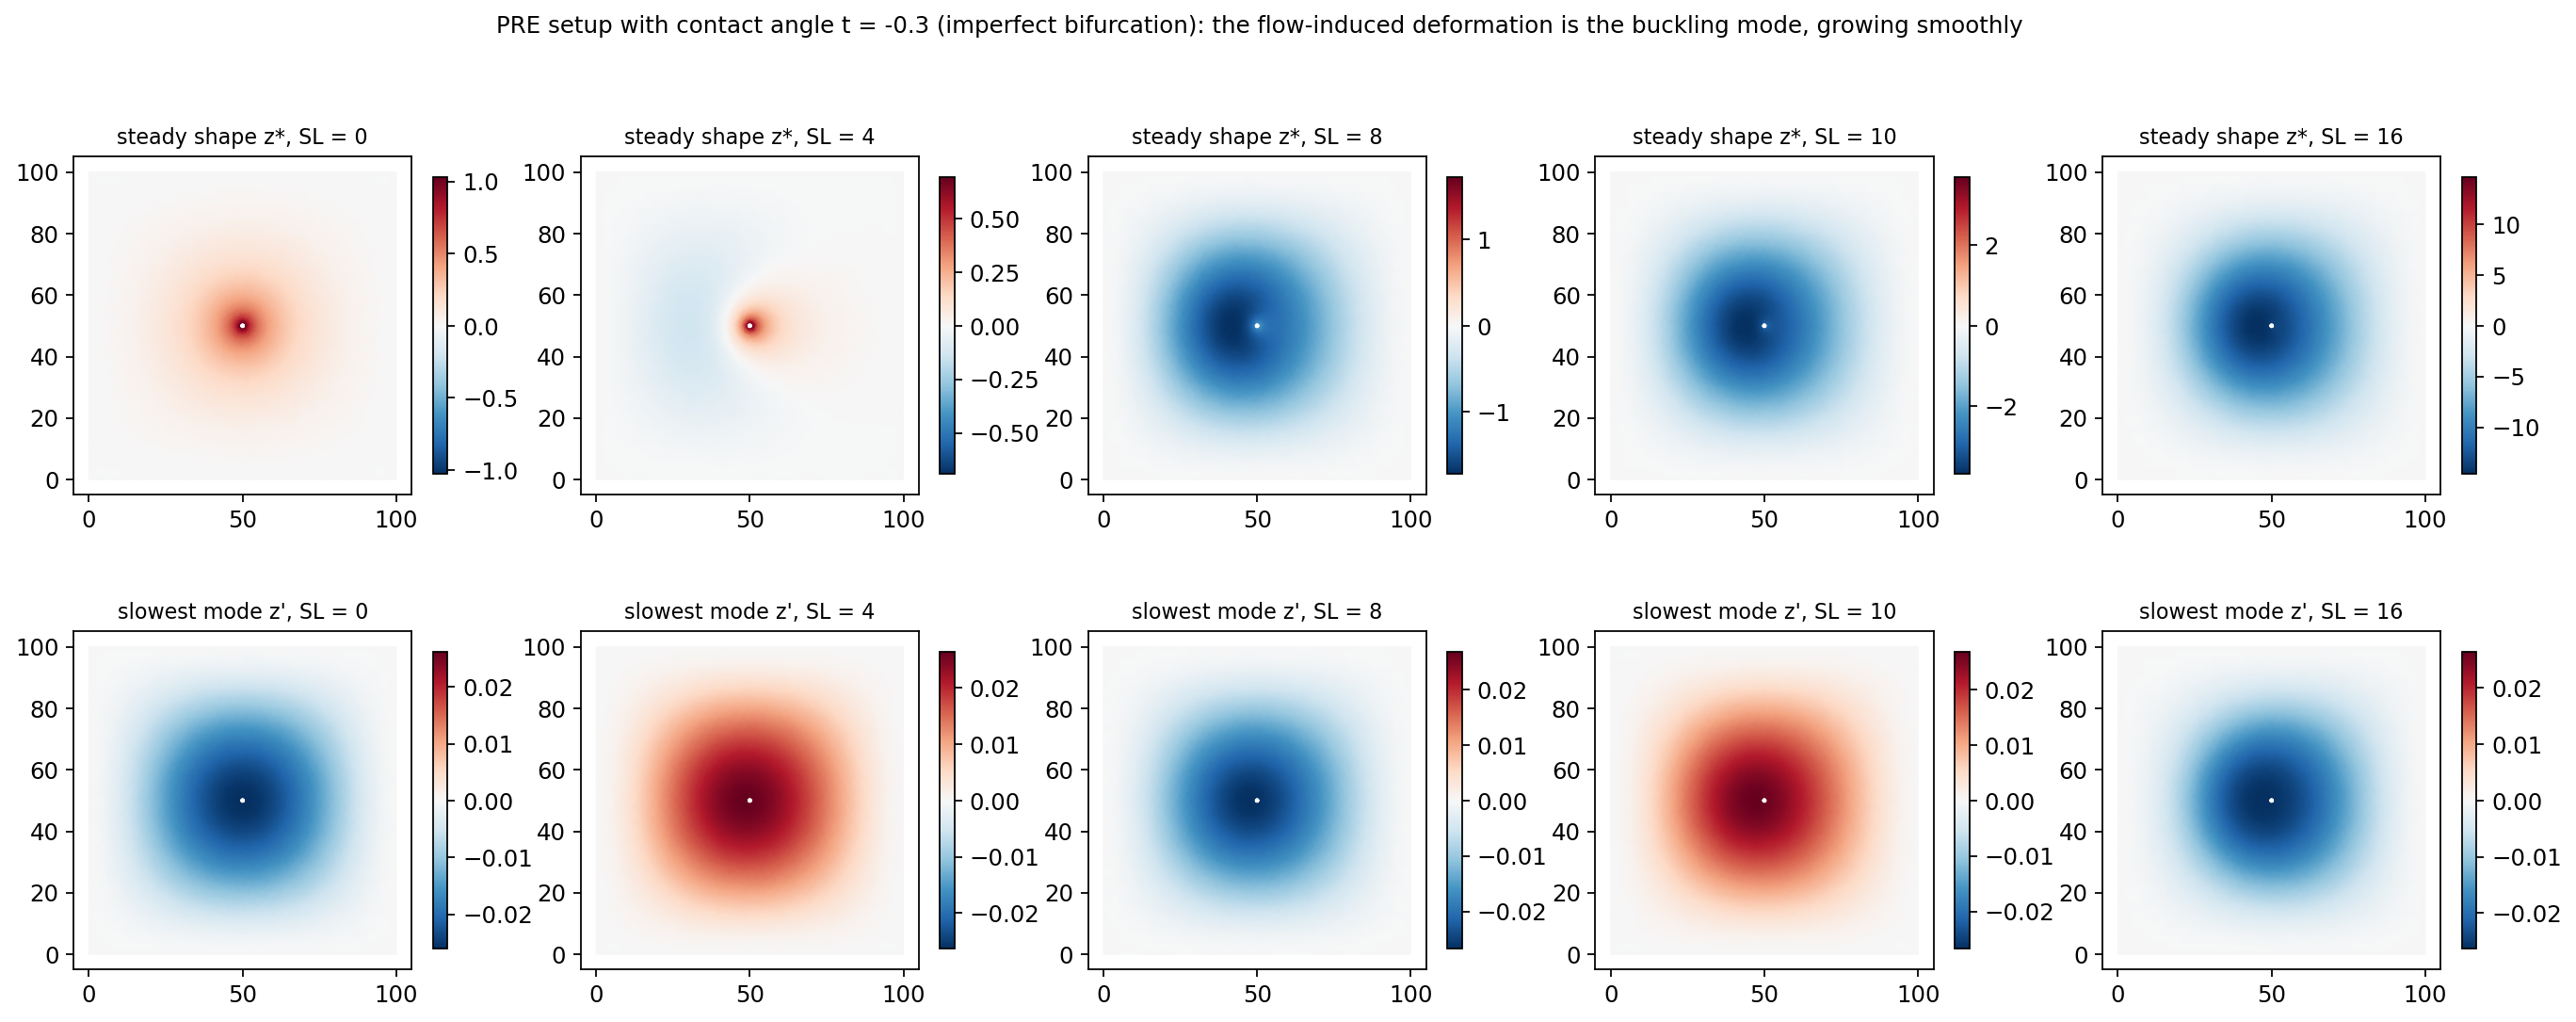
\includegraphics[width=\linewidth,height=86mm,keepaspectratio]{figures/membrane_flow_pre_imperfect_shapes.png}\captionof{figure}[Archived figure]{Superseded original-rim shapes and leading modes at nonzero contact slope. Their large smooth deformation is not evidence for a smooth transition with a physically force-free protein. \textit{Source:} \path{Ruben/membrane_stability/figures/flow_pre_imperfect_shapes.png}. First added 2026-09-30.}\end{center}
\clearpage
\begin{center}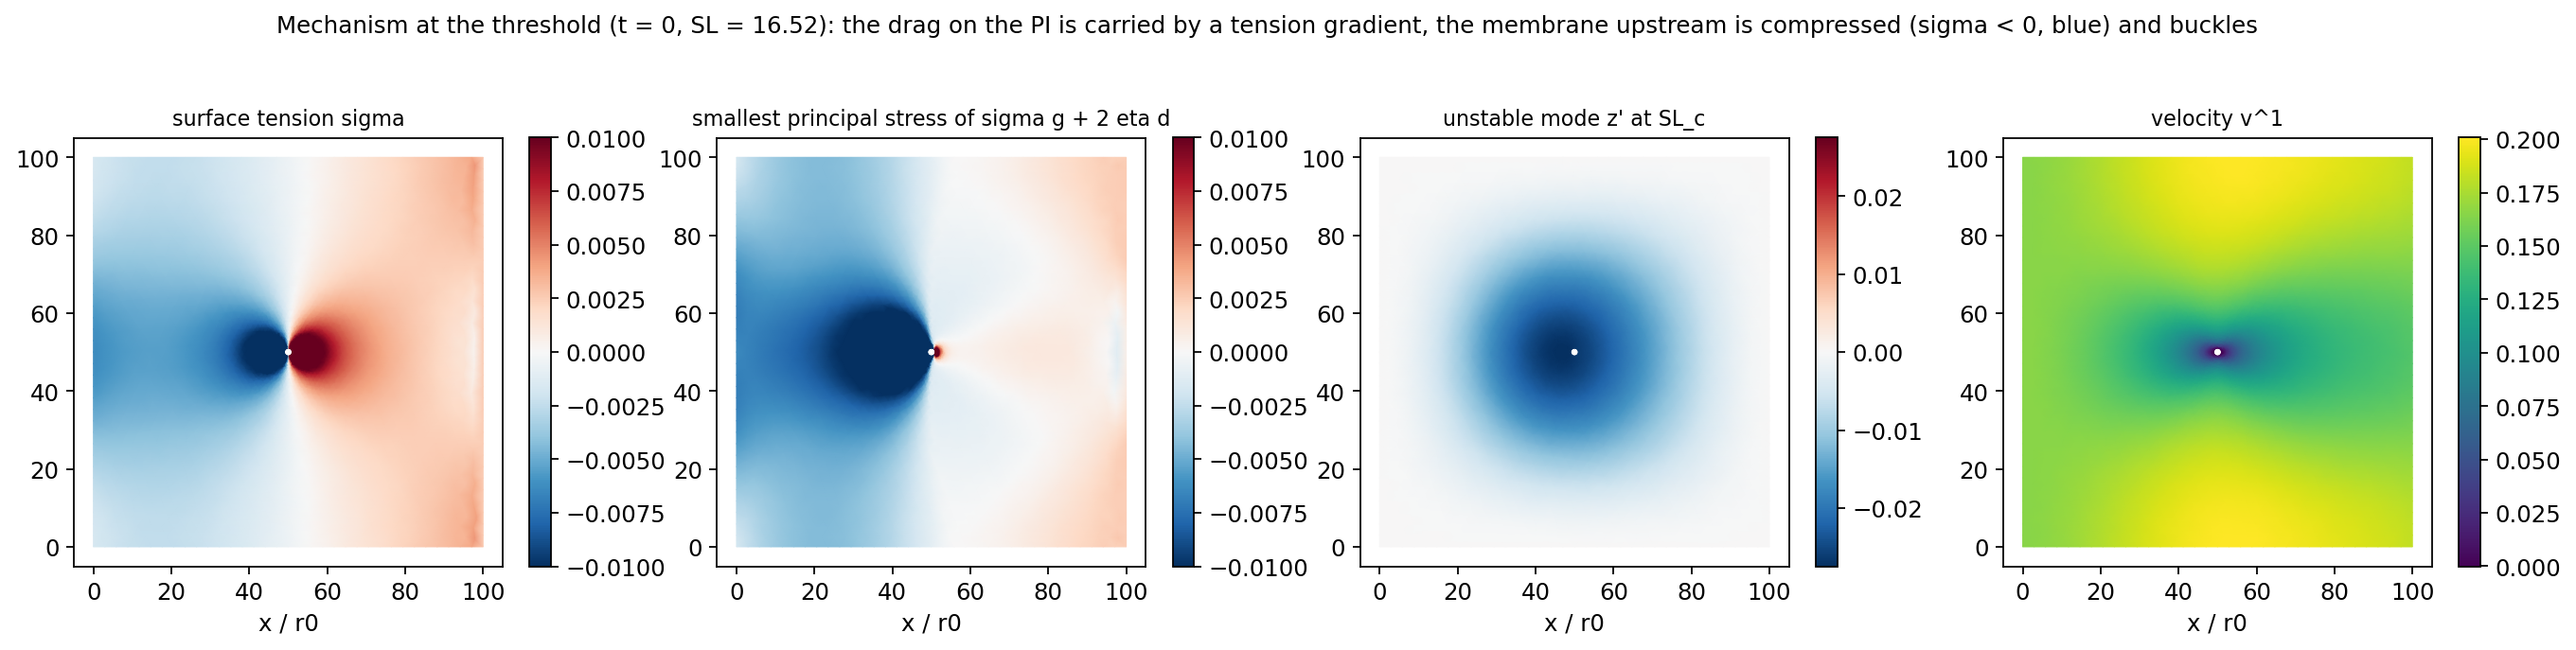
\includegraphics[width=\linewidth,height=86mm,keepaspectratio]{figures/membrane_flow_pre_mechanism.png}\captionof{figure}[Archived figure]{Superseded original-rim stress and eigenmode fields. They reveal upstream compression but place the mode nearer the protein than the corrected force-balanced problem. \textit{Source:} \path{Ruben/membrane_stability/figures/flow_pre_mechanism.png}. First added 2026-09-30.}\end{center}
\begin{center}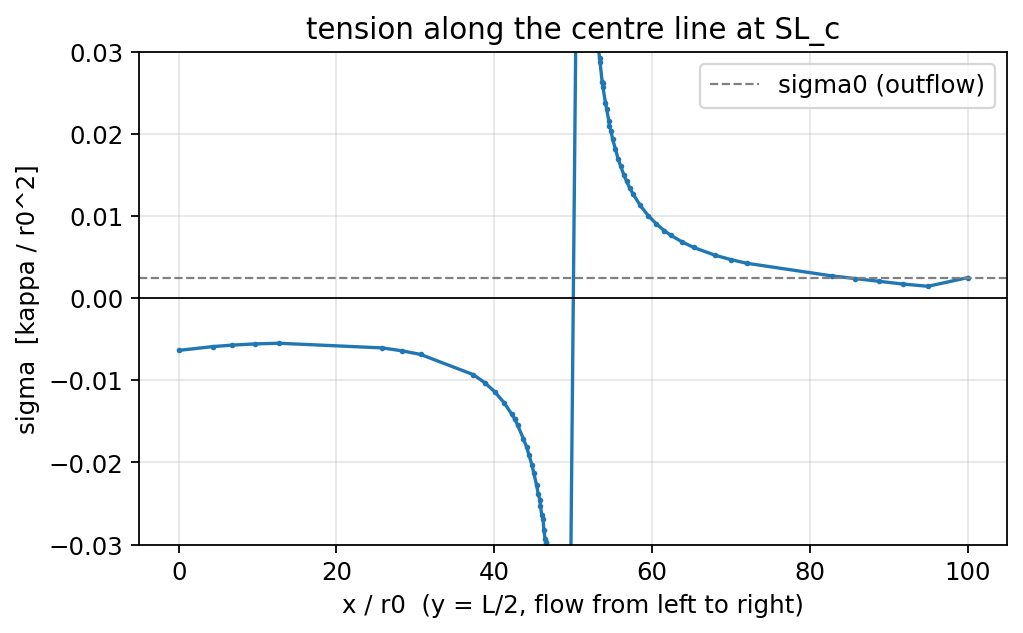
\includegraphics[width=\linewidth,height=86mm,keepaspectratio]{figures/membrane_flow_pre_tension_centreline.png}\captionof{figure}[Archived figure]{Original-rim flat base-flow tension along the centreline. The upstream tension decrease is mechanistic evidence; the onset value attached to this figure is superseded by the physical protein condition. \textit{Source:} \path{Ruben/membrane_stability/figures/flow_pre_tension_centreline.png}. First added 2026-09-30.}\end{center}
\clearpage
\begin{center}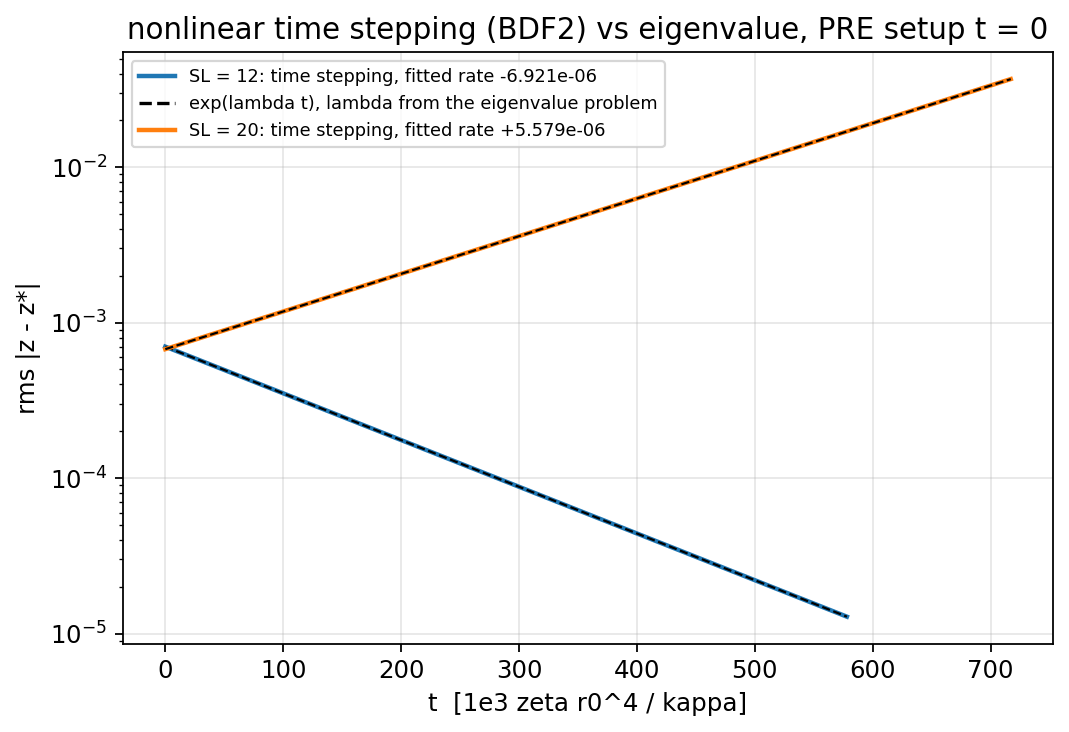
\includegraphics[width=\linewidth,height=182mm,keepaspectratio]{figures/membrane_flow_time_check.png}\captionof{figure}[Archived figure]{BDF2 versus eigenvalue growth and decay for the original-rim implementation. This checks that the numerical linearization predicts that implementation's dynamics, not that its rim condition is physically force-free. \textit{Source:} \path{Ruben/membrane_stability/figures/flow_time_check.png}. First added 2026-09-30.}\end{center}
\clearpage
\begin{center}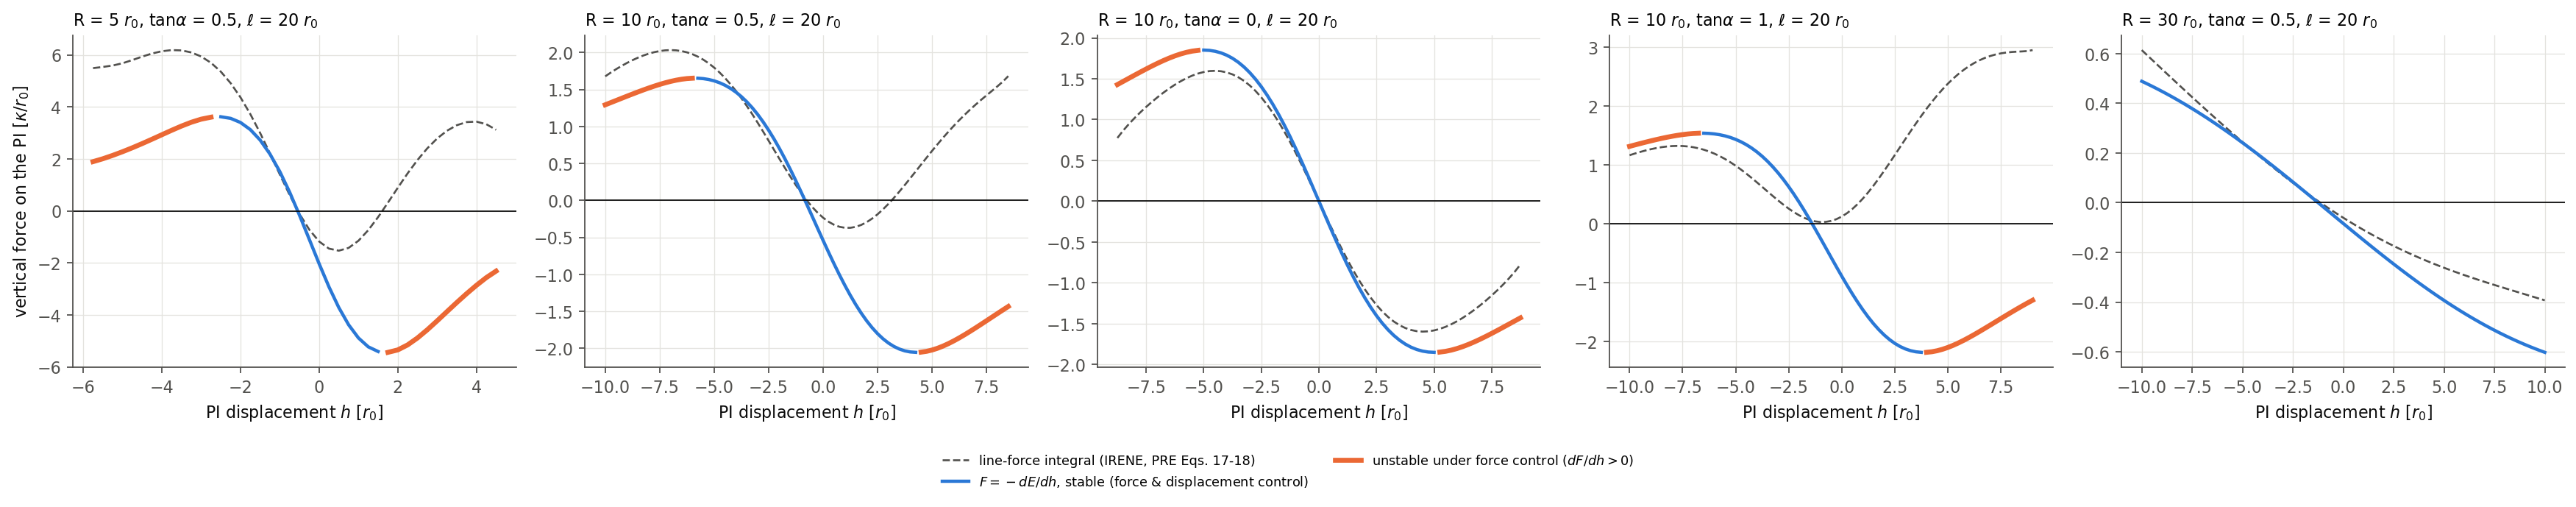
\includegraphics[width=\linewidth,height=86mm,keepaspectratio]{figures/membrane_force_displacement.png}\captionof{figure}[Archived figure]{Ring forces and fixed-height eigenvalues for several radii. Dashed original line-force curves are retained as diagnostics; extrema and force-control conclusions use virtual work. \textit{Source:} \path{Ruben/membrane_stability/figures/force_displacement.png}. First added 2026-09-29.}\end{center}
\begin{center}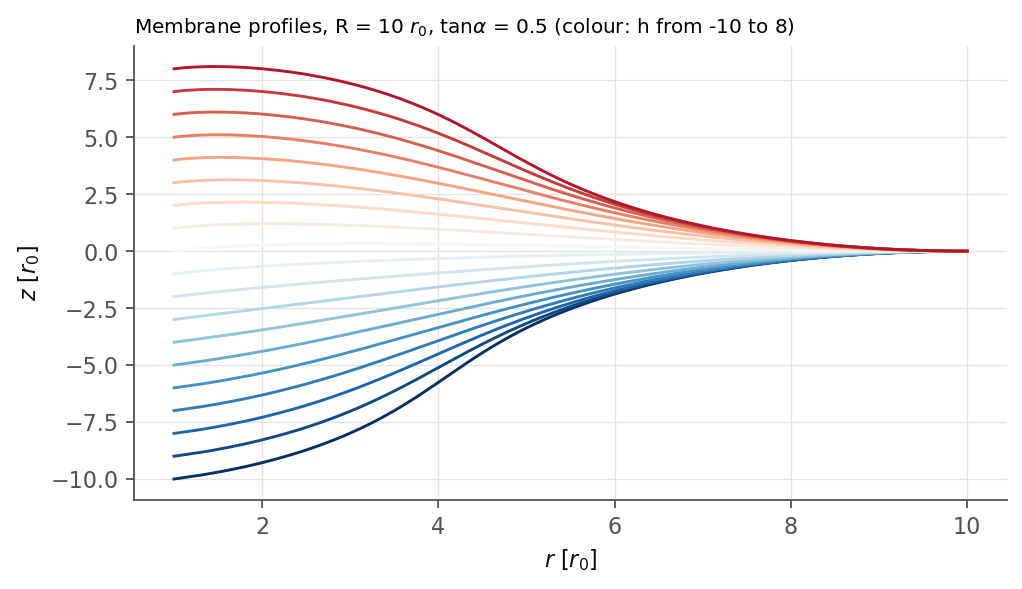
\includegraphics[width=\linewidth,height=86mm,keepaspectratio]{figures/membrane_profiles_ring_R10_tan0.5.png}\captionof{figure}[Archived figure]{Ring profiles for outer radius ten and contact slope one half. Increasing imposed height produces a steep neck while the corresponding fixed-height spectrum remains stable in the sampled range. \textit{Source:} \path{Ruben/membrane_stability/figures/profiles_ring_R10_tan0.5.png}. First added 2026-09-29.}\end{center}
\clearpage
\begin{center}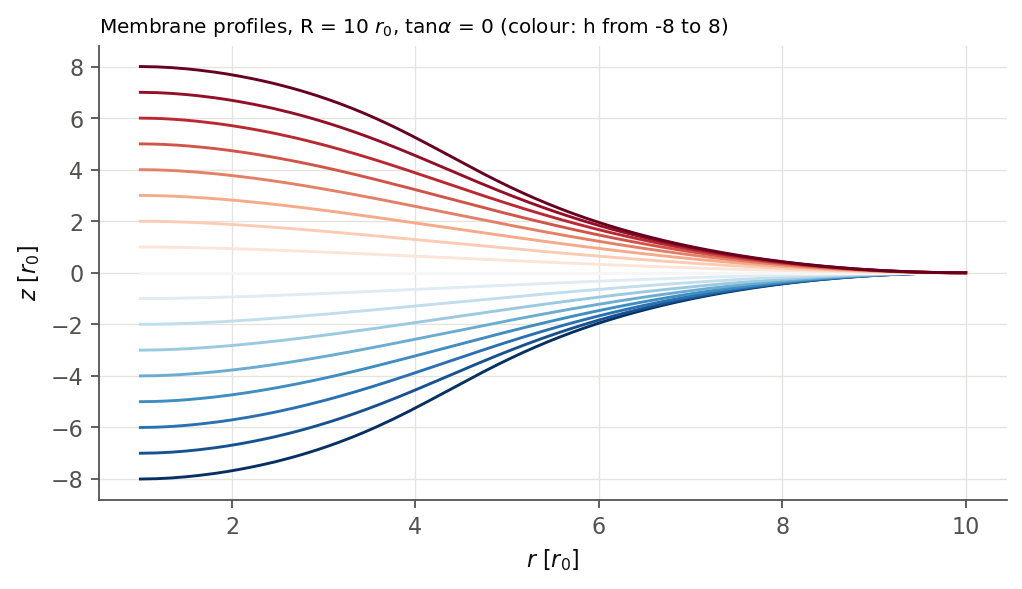
\includegraphics[width=\linewidth,height=182mm,keepaspectratio]{figures/membrane_profiles_ring_R10_tan0.png}\captionof{figure}[Archived figure]{Symmetric zero-contact-slope ring profiles at outer radius ten. Upward and downward branches are related by reflection in the reference plane. \textit{Source:} \path{Ruben/membrane_stability/figures/profiles_ring_R10_tan0.png}. First added 2026-09-29.}\end{center}
\clearpage
\begin{center}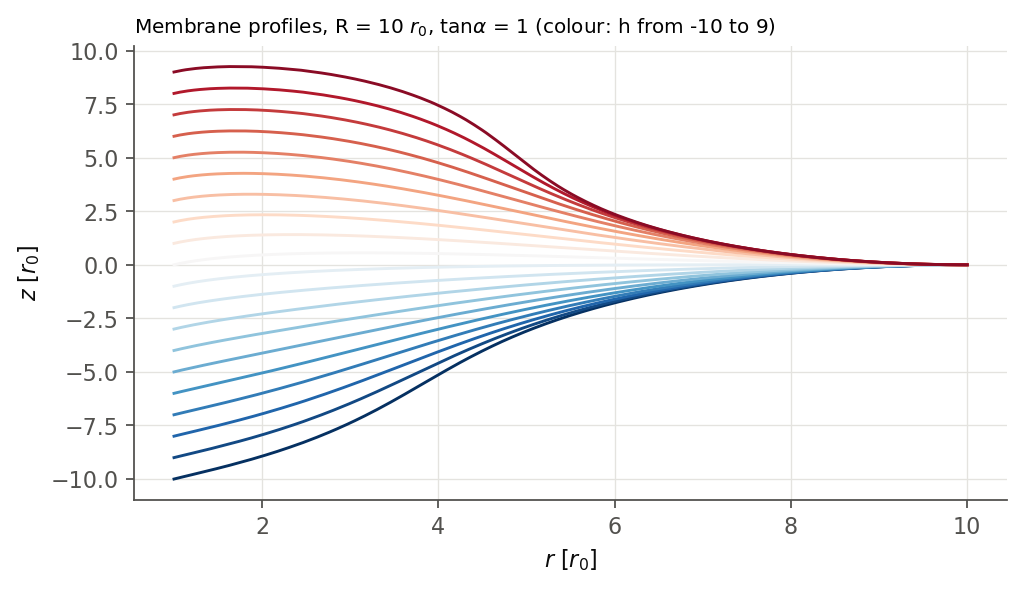
\includegraphics[width=\linewidth,height=182mm,keepaspectratio]{figures/membrane_profiles_ring_R10_tan1.png}\captionof{figure}[Archived figure]{Ring profiles at outer radius ten and unit contact slope. The imposed slope biases the spontaneous height and the two force-control barriers. \textit{Source:} \path{Ruben/membrane_stability/figures/profiles_ring_R10_tan1.png}. First added 2026-09-29.}\end{center}
\clearpage
\begin{center}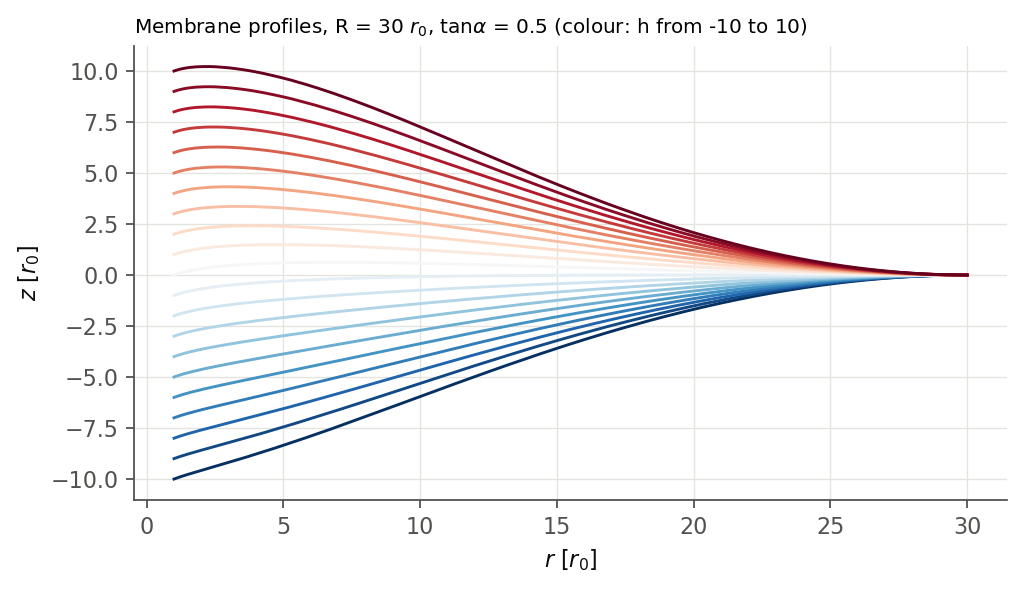
\includegraphics[width=\linewidth,height=182mm,keepaspectratio]{figures/membrane_profiles_ring_R30_tan0.5.png}\captionof{figure}[Archived figure]{Profiles for outer radius thirty and contact slope one half. The displayed Monge window does not reach the long-tube force plateau. \textit{Source:} \path{Ruben/membrane_stability/figures/profiles_ring_R30_tan0.5.png}. First added 2026-09-29.}\end{center}
\clearpage
\begin{center}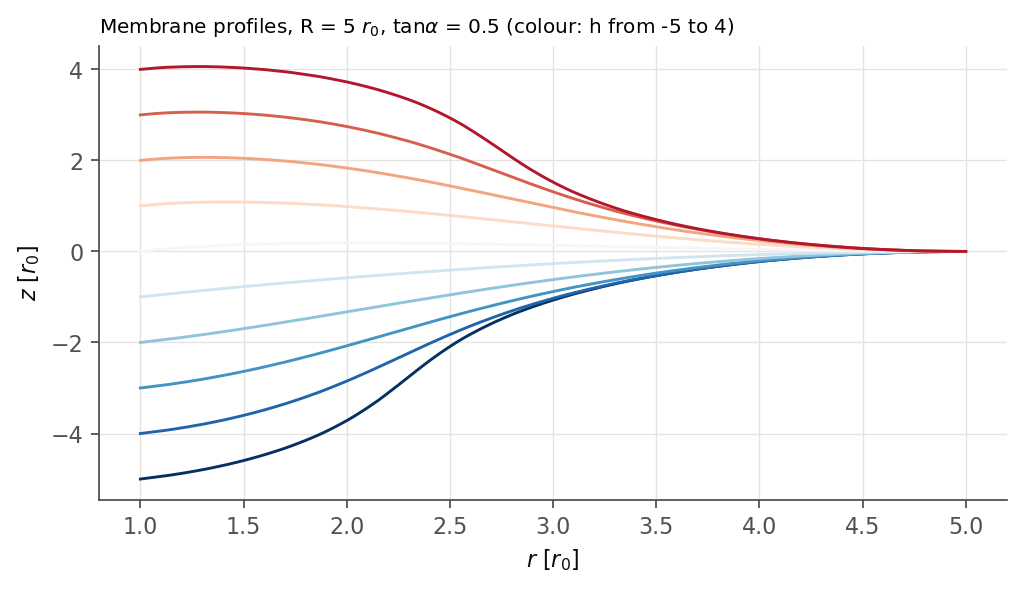
\includegraphics[width=\linewidth,height=86mm,keepaspectratio]{figures/membrane_profiles_ring_R5_tan0.5.png}\captionof{figure}[Archived figure]{Strongly confined ring profiles at outer radius five. Large end slopes limit a height representation and distinguish the confined neck from a freely developed wide tube. \textit{Source:} \path{Ruben/membrane_stability/figures/profiles_ring_R5_tan0.5.png}. First added 2026-09-29.}\end{center}
\begin{center}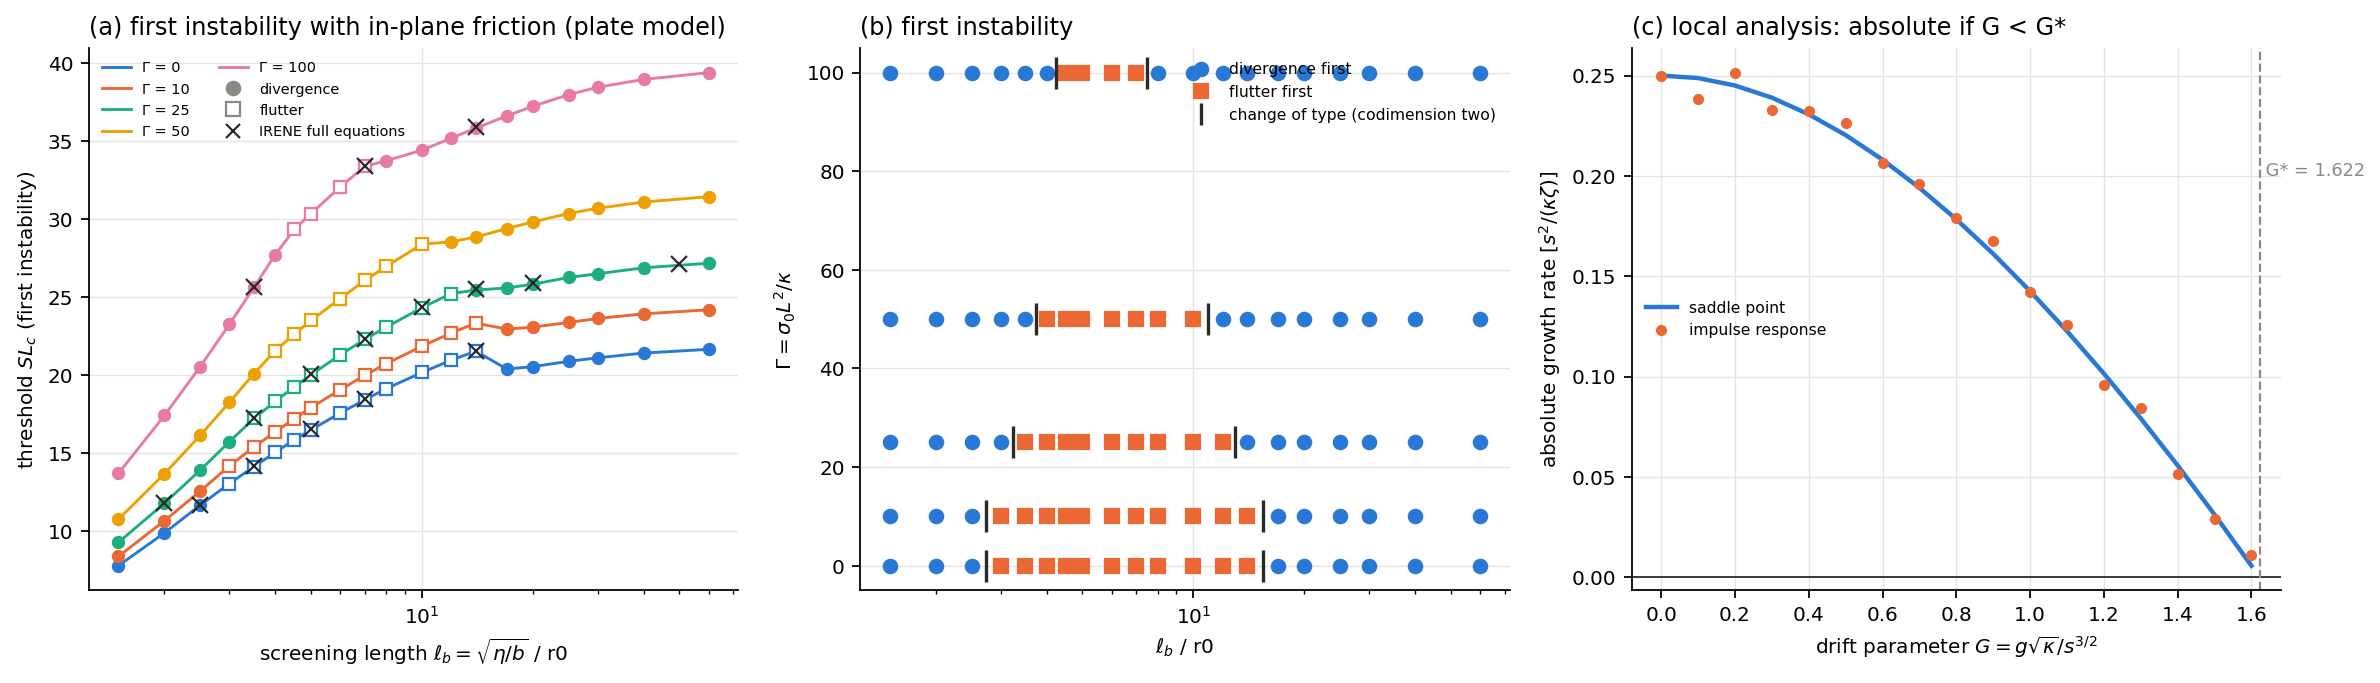
\includegraphics[width=\linewidth,height=86mm,keepaspectratio]{figures/membrane_r3_flutter_map.png}\captionof{figure}[Archived figure]{Divergence/flutter onset map versus screening length and tension, with full-equation checks. The local absolute-instability panel is a guide to the global wave source; near onset the local wavelength is comparable to the compressed region. \textit{Source:} \path{Ruben/membrane_stability/figures/r3_flutter_map.png}. First added 2026-10-01.}\end{center}
\clearpage
\begin{center}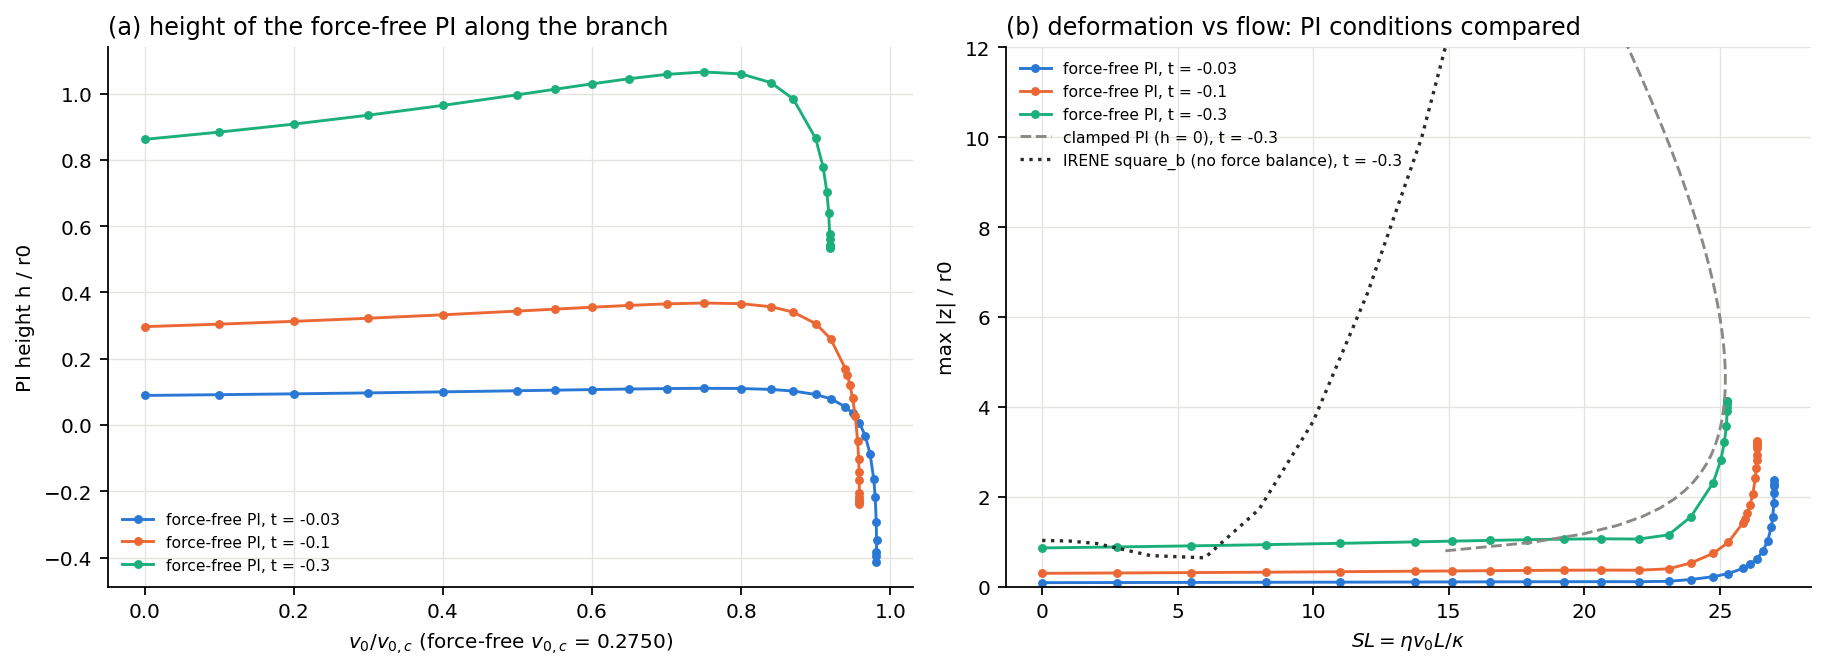
\includegraphics[width=\linewidth,height=182mm,keepaspectratio]{figures/membrane_r3_forcefree.png}\captionof{figure}[Archived figure]{Nonlinear force-free branches for nonzero contact slopes, contrasted with clamped and original-rim conditions. The corrected free protein stays near its rest deformation before an imperfection-sensitive fold. \textit{Source:} \path{Ruben/membrane_stability/figures/r3_forcefree.png}. First added 2026-10-01.}\end{center}
\clearpage
\begin{center}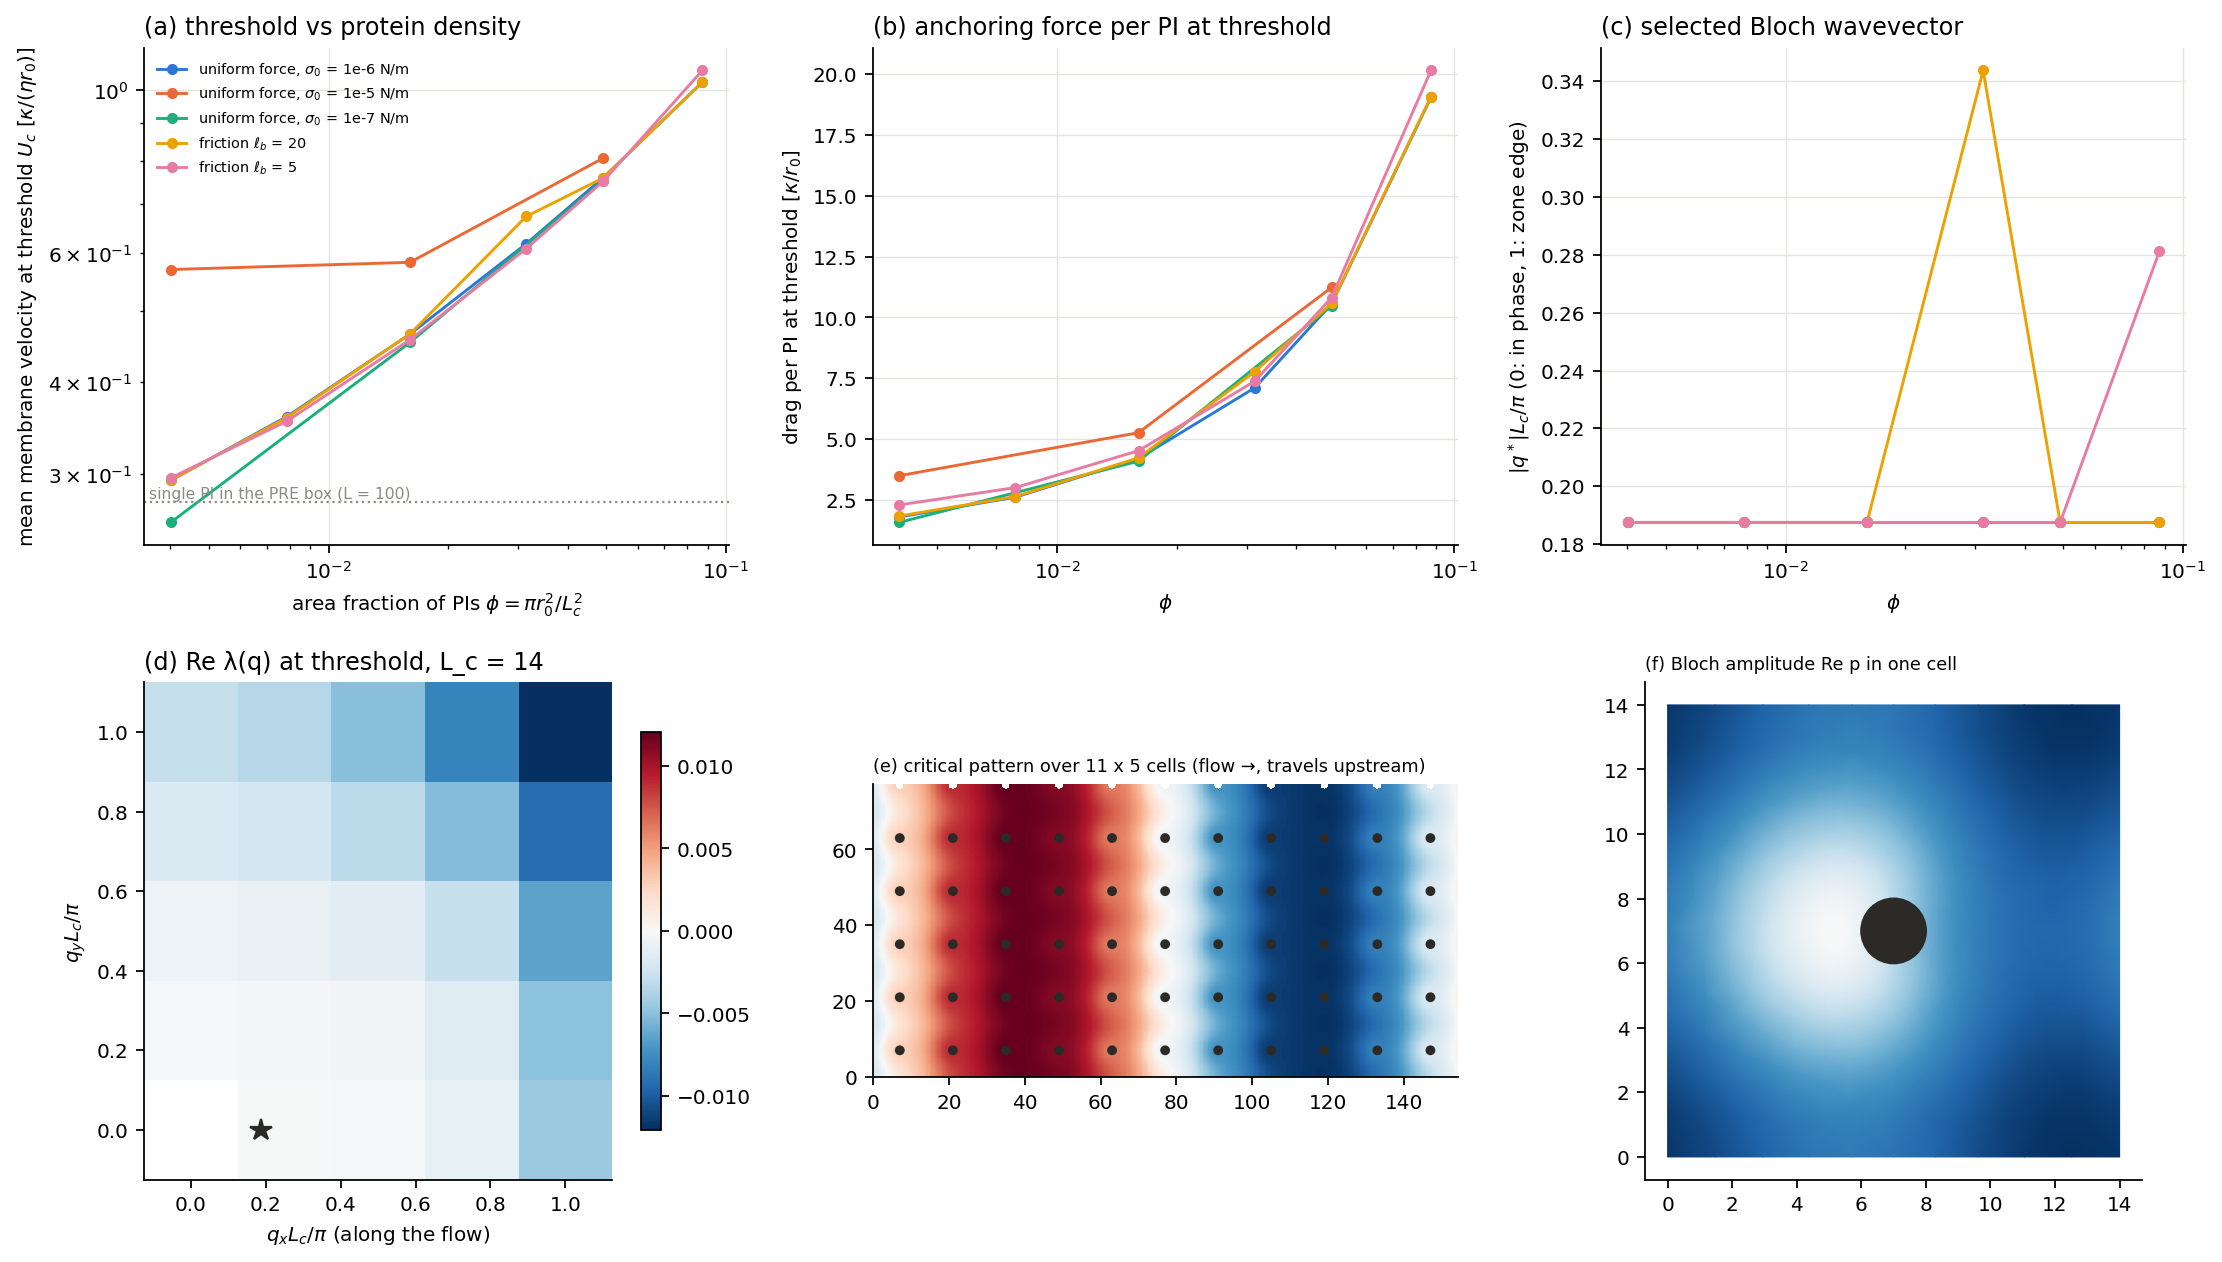
\includegraphics[width=\linewidth,height=182mm,keepaspectratio]{figures/membrane_r3_lattice.png}\captionof{figure}[Archived figure]{Periodic array spectra and patterns. Early finite-wavevector scans are interpreted with the dedicated later long-wave coefficients: a neutral uniform translation exists at zero wavevector, and the longitudinal stiffness controls onset. \textit{Source:} \path{Ruben/membrane_stability/figures/r3_lattice.png}. First added 2026-10-01.}\end{center}
\clearpage
\begin{center}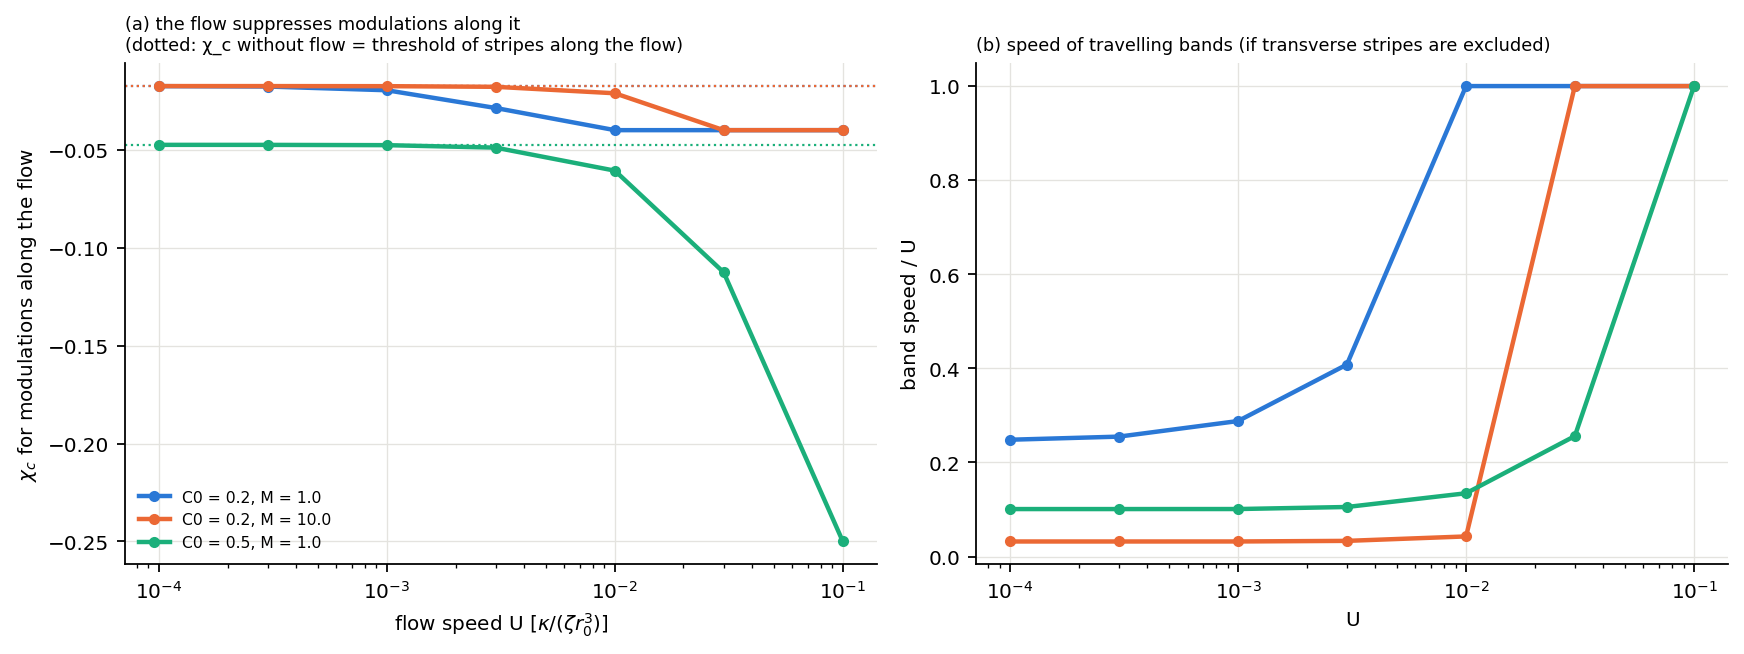
\includegraphics[width=\linewidth,height=182mm,keepaspectratio]{figures/membrane_r3_mobile.png}\captionof{figure}[Archived figure]{Uniform-plane curvature-protein dispersion under relative drift. Transverse wavevectors remain least affected, giving stripes parallel to the flow; travelling longitudinal bands require suppressing those transverse modes. \textit{Source:} \path{Ruben/membrane_stability/figures/r3_mobile.png}. First added 2026-10-01.}\end{center}
\clearpage
\begin{center}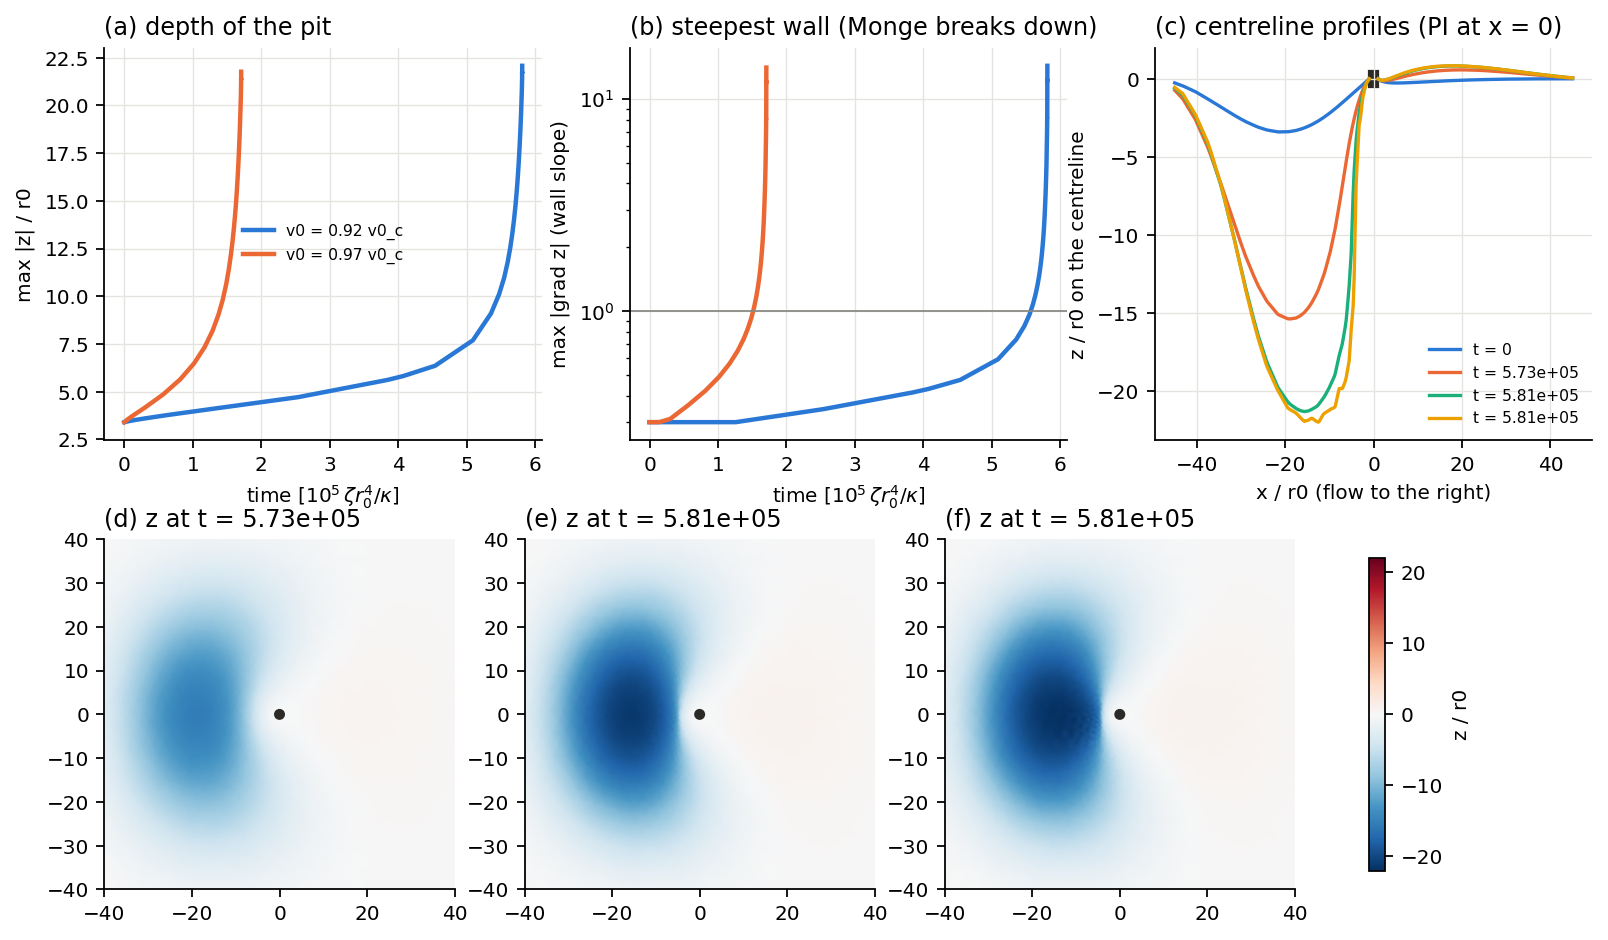
\includegraphics[width=\linewidth,height=182mm,keepaspectratio]{figures/membrane_r3_snap.png}\captionof{figure}[Archived figure]{Clamped-protein time stepping after the fold: bottleneck, deepening upstream pit, and rapid slope growth. The final steep shapes are at the Monge limit, not resolved steady attractors. \textit{Source:} \path{Ruben/membrane_stability/figures/r3_snap.png}. First added 2026-10-01.}\end{center}
\clearpage
\begin{center}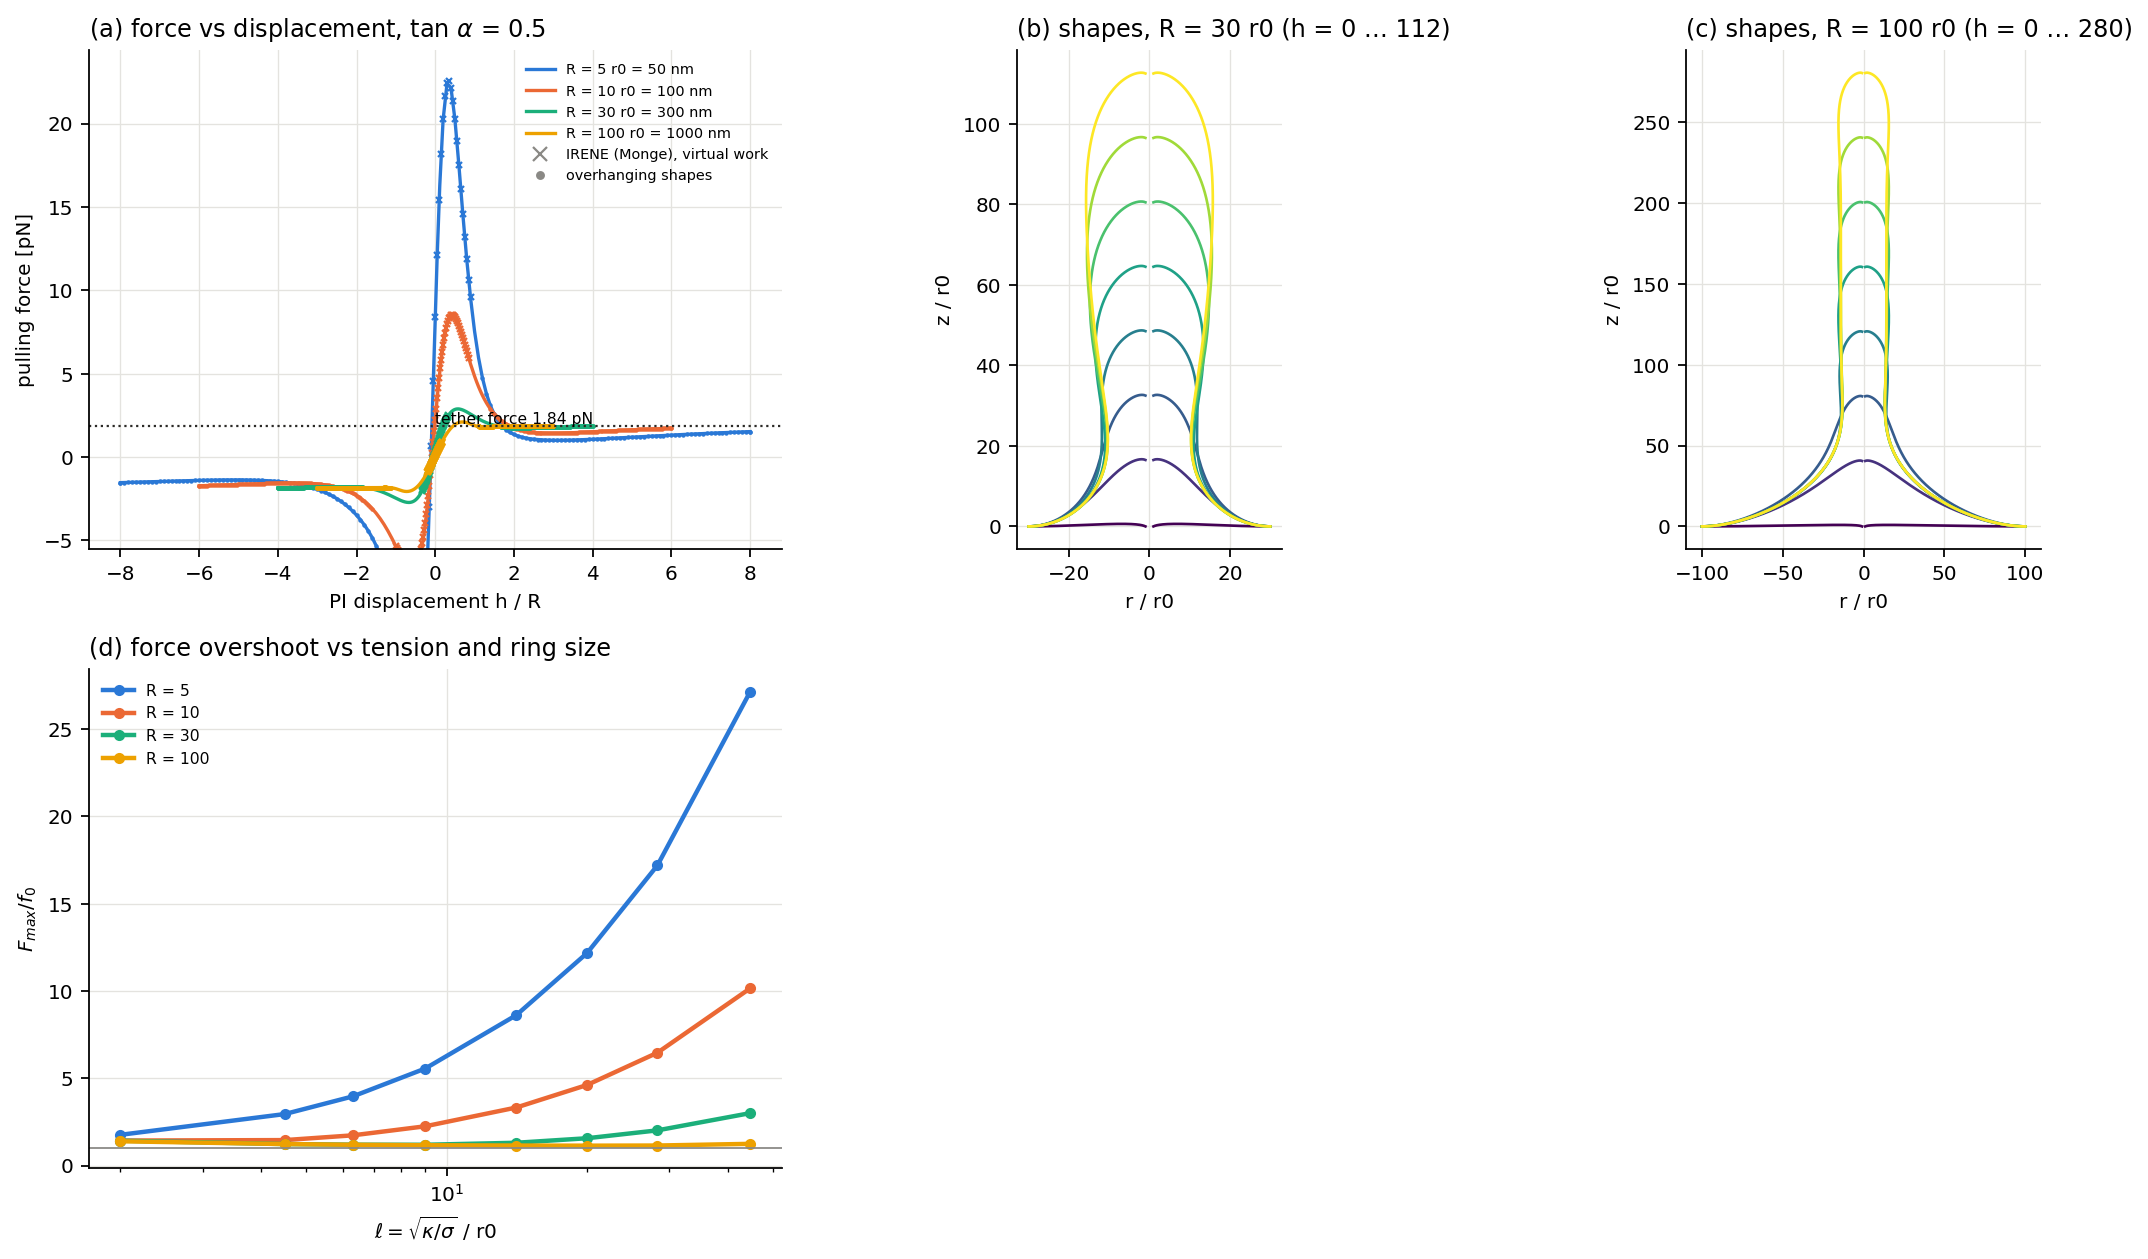
\includegraphics[width=\linewidth,height=182mm,keepaspectratio]{figures/membrane_r3_tube.png}\captionof{figure}[Archived figure]{No-flow axisymmetric arclength continuation. Large rings develop tubes tending to the tether-force plateau; small rings constrain a neck and show a large force overshoot. This is distinct from flow-driven tube growth, which remains unfinished. \textit{Source:} \path{Ruben/membrane_stability/figures/r3_tube.png}. First added 2026-10-01.}\end{center}
\clearpage
\begin{center}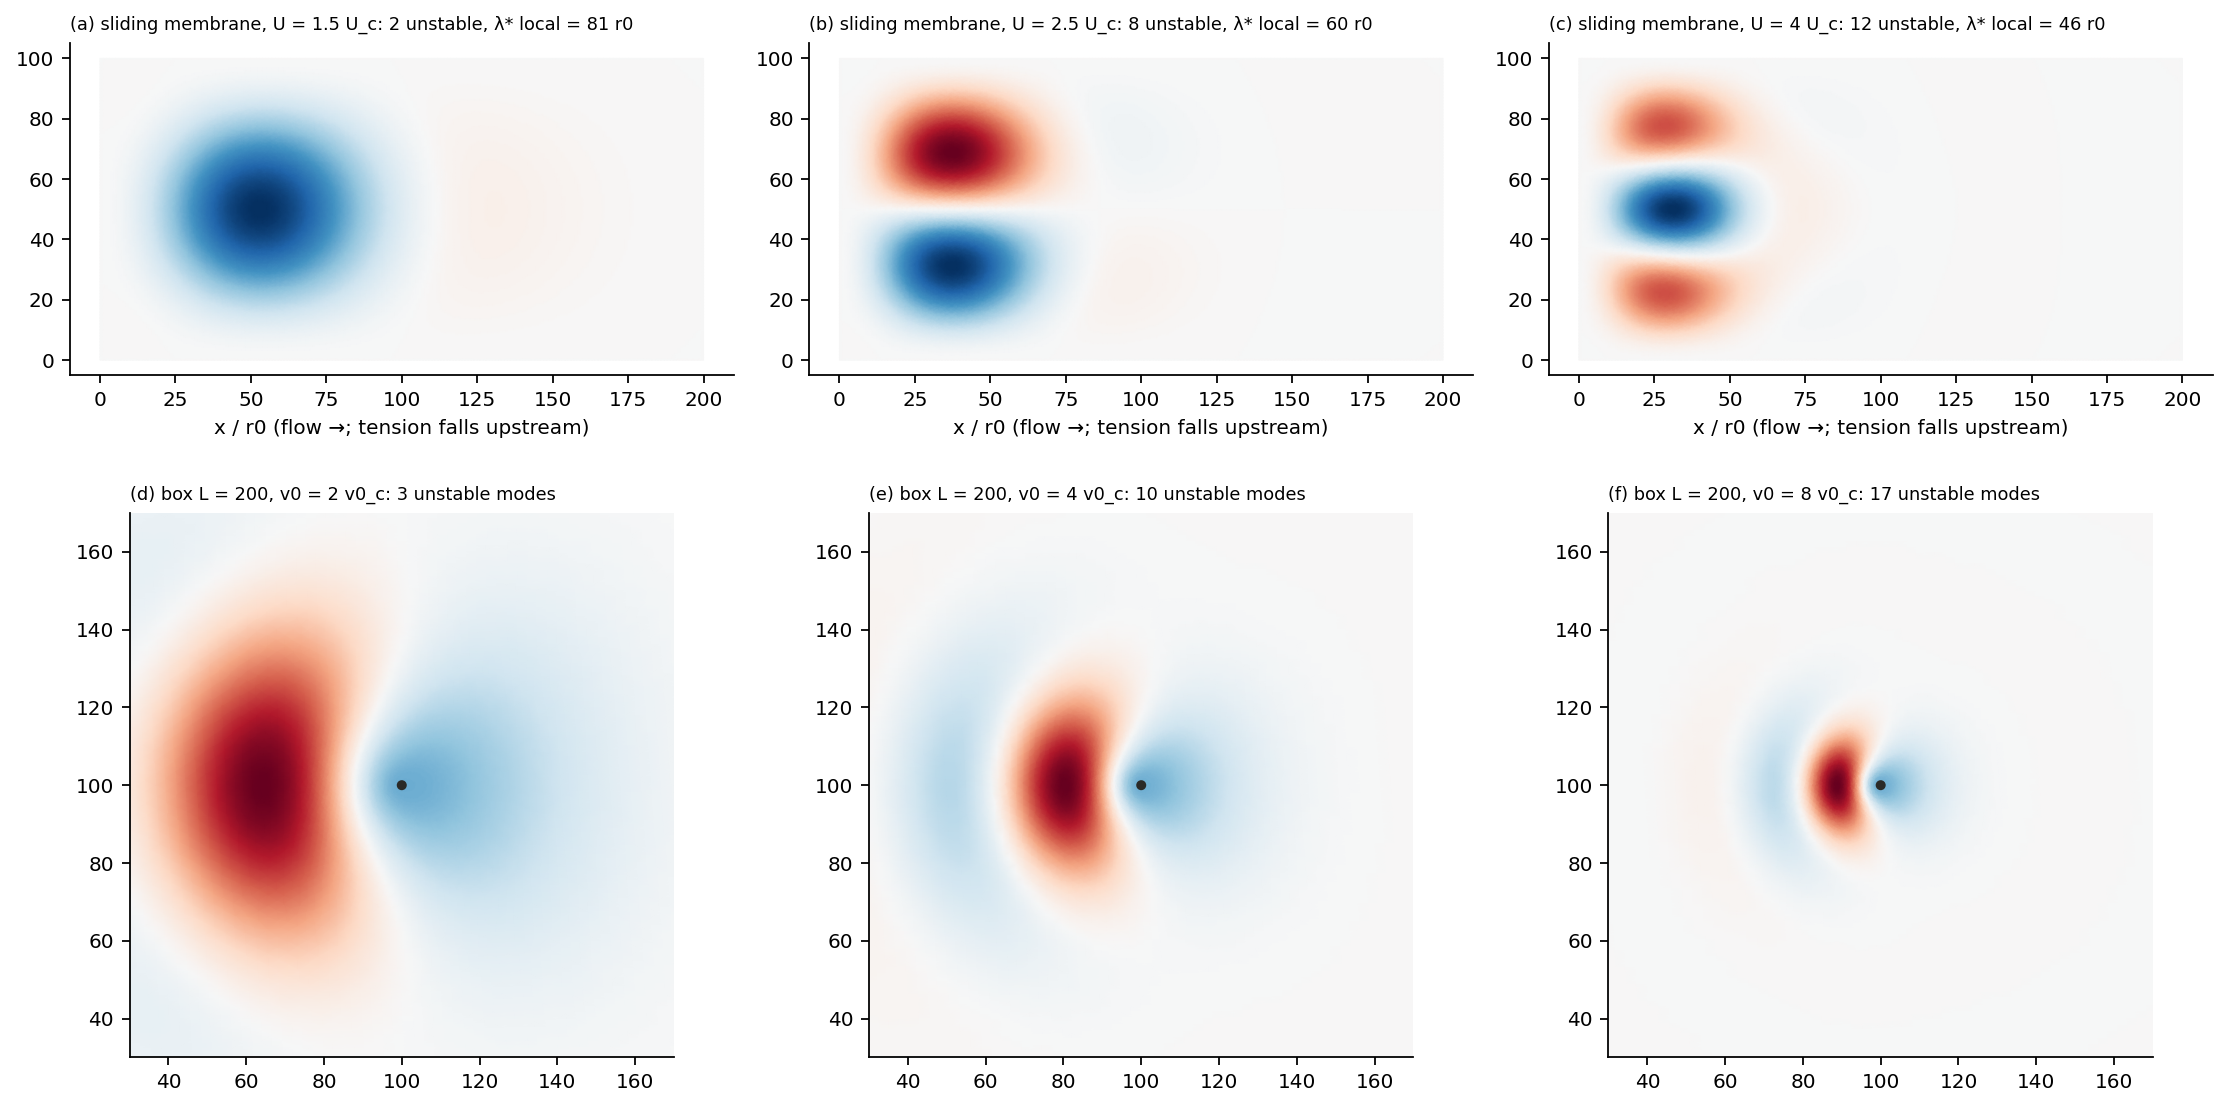
\includegraphics[width=\linewidth,height=86mm,keepaspectratio]{figures/membrane_r3_wrinkles.png}\captionof{figure}[Archived figure]{Plate-model modes well above onset and in sliding-membrane examples. Increasing compression permits multiple lobes and wrinkle trains; these modes do not establish a stable nonlinear pattern around a single protein. \textit{Source:} \path{Ruben/membrane_stability/figures/r3_wrinkles.png}. First added 2026-10-01.}\end{center}
\begin{center}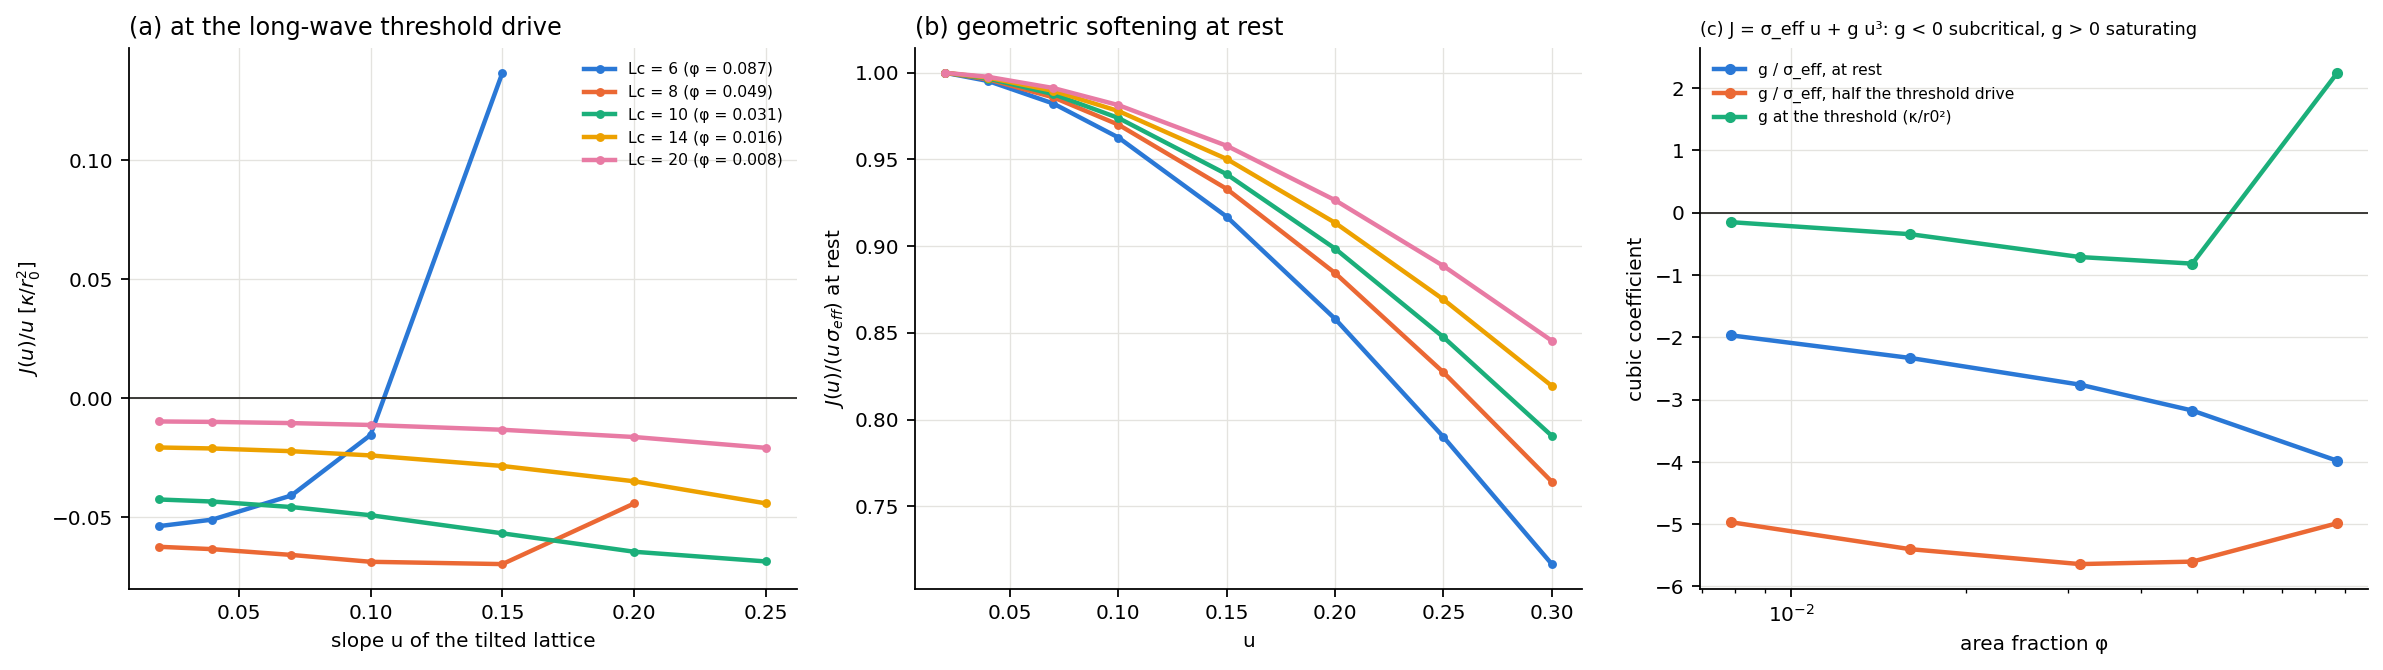
\includegraphics[width=\linewidth,height=86mm,keepaspectratio]{figures/membrane_r4_lattice_nonlinear.png}\captionof{figure}[Archived figure]{Nonlinear tilted-cell stress and geometric softening. Frozen flat-state flow is used; the small-slope cubic changes sign between intermediate and dense arrays, while the driven linear coefficient differs modestly from the dynamic Bloch value. \textit{Source:} \path{Ruben/membrane_stability/figures/r4_lattice_nonlinear.png}. First added 2026-10-01.}\end{center}
\clearpage
\begin{center}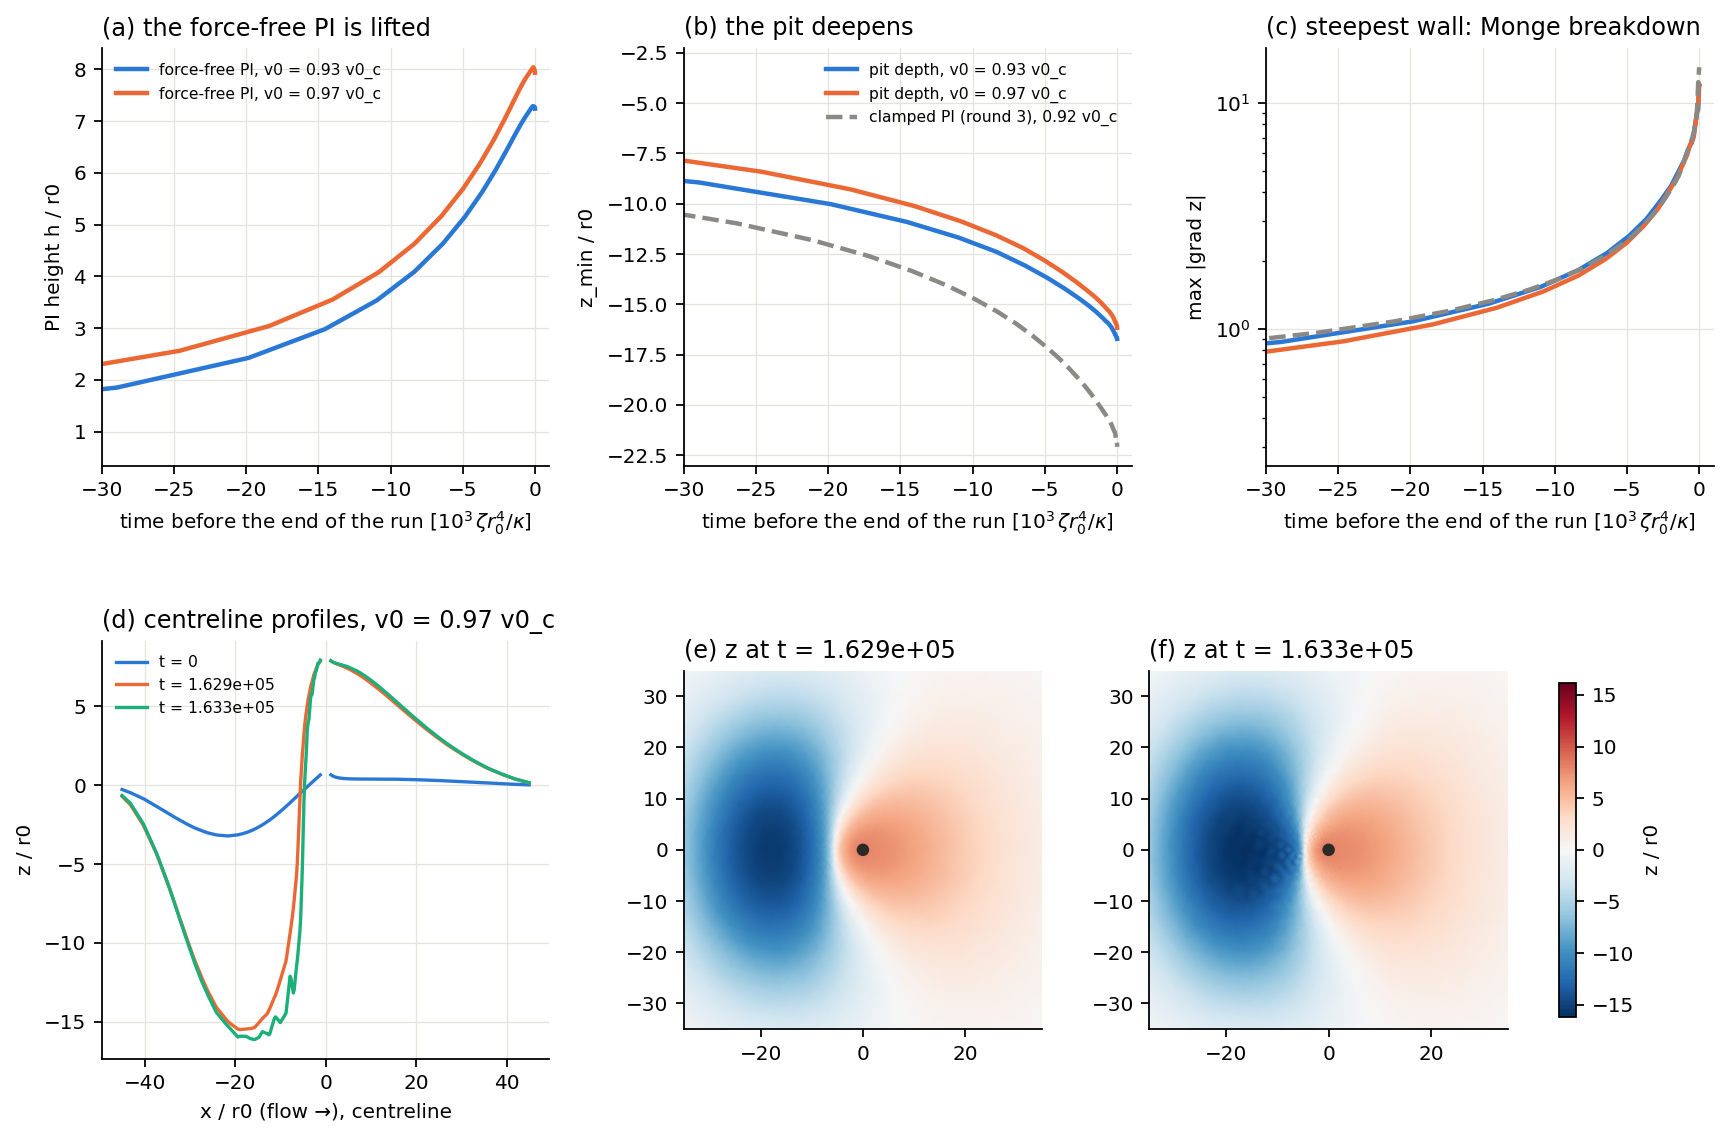
\includegraphics[width=\linewidth,height=182mm,keepaspectratio]{figures/membrane_r4_post_snap_forcefree.png}\captionof{figure}[Archived figure]{Force-free protein lift during upstream collapse. The protein rises onto a downstream crest and the wall steepens; cutoff-force consistency deteriorates at the last slopes. \textit{Source:} \path{Ruben/membrane_stability/figures/r4_post_snap_forcefree.png}. First added 2026-10-01.}\end{center}
\clearpage
\begin{center}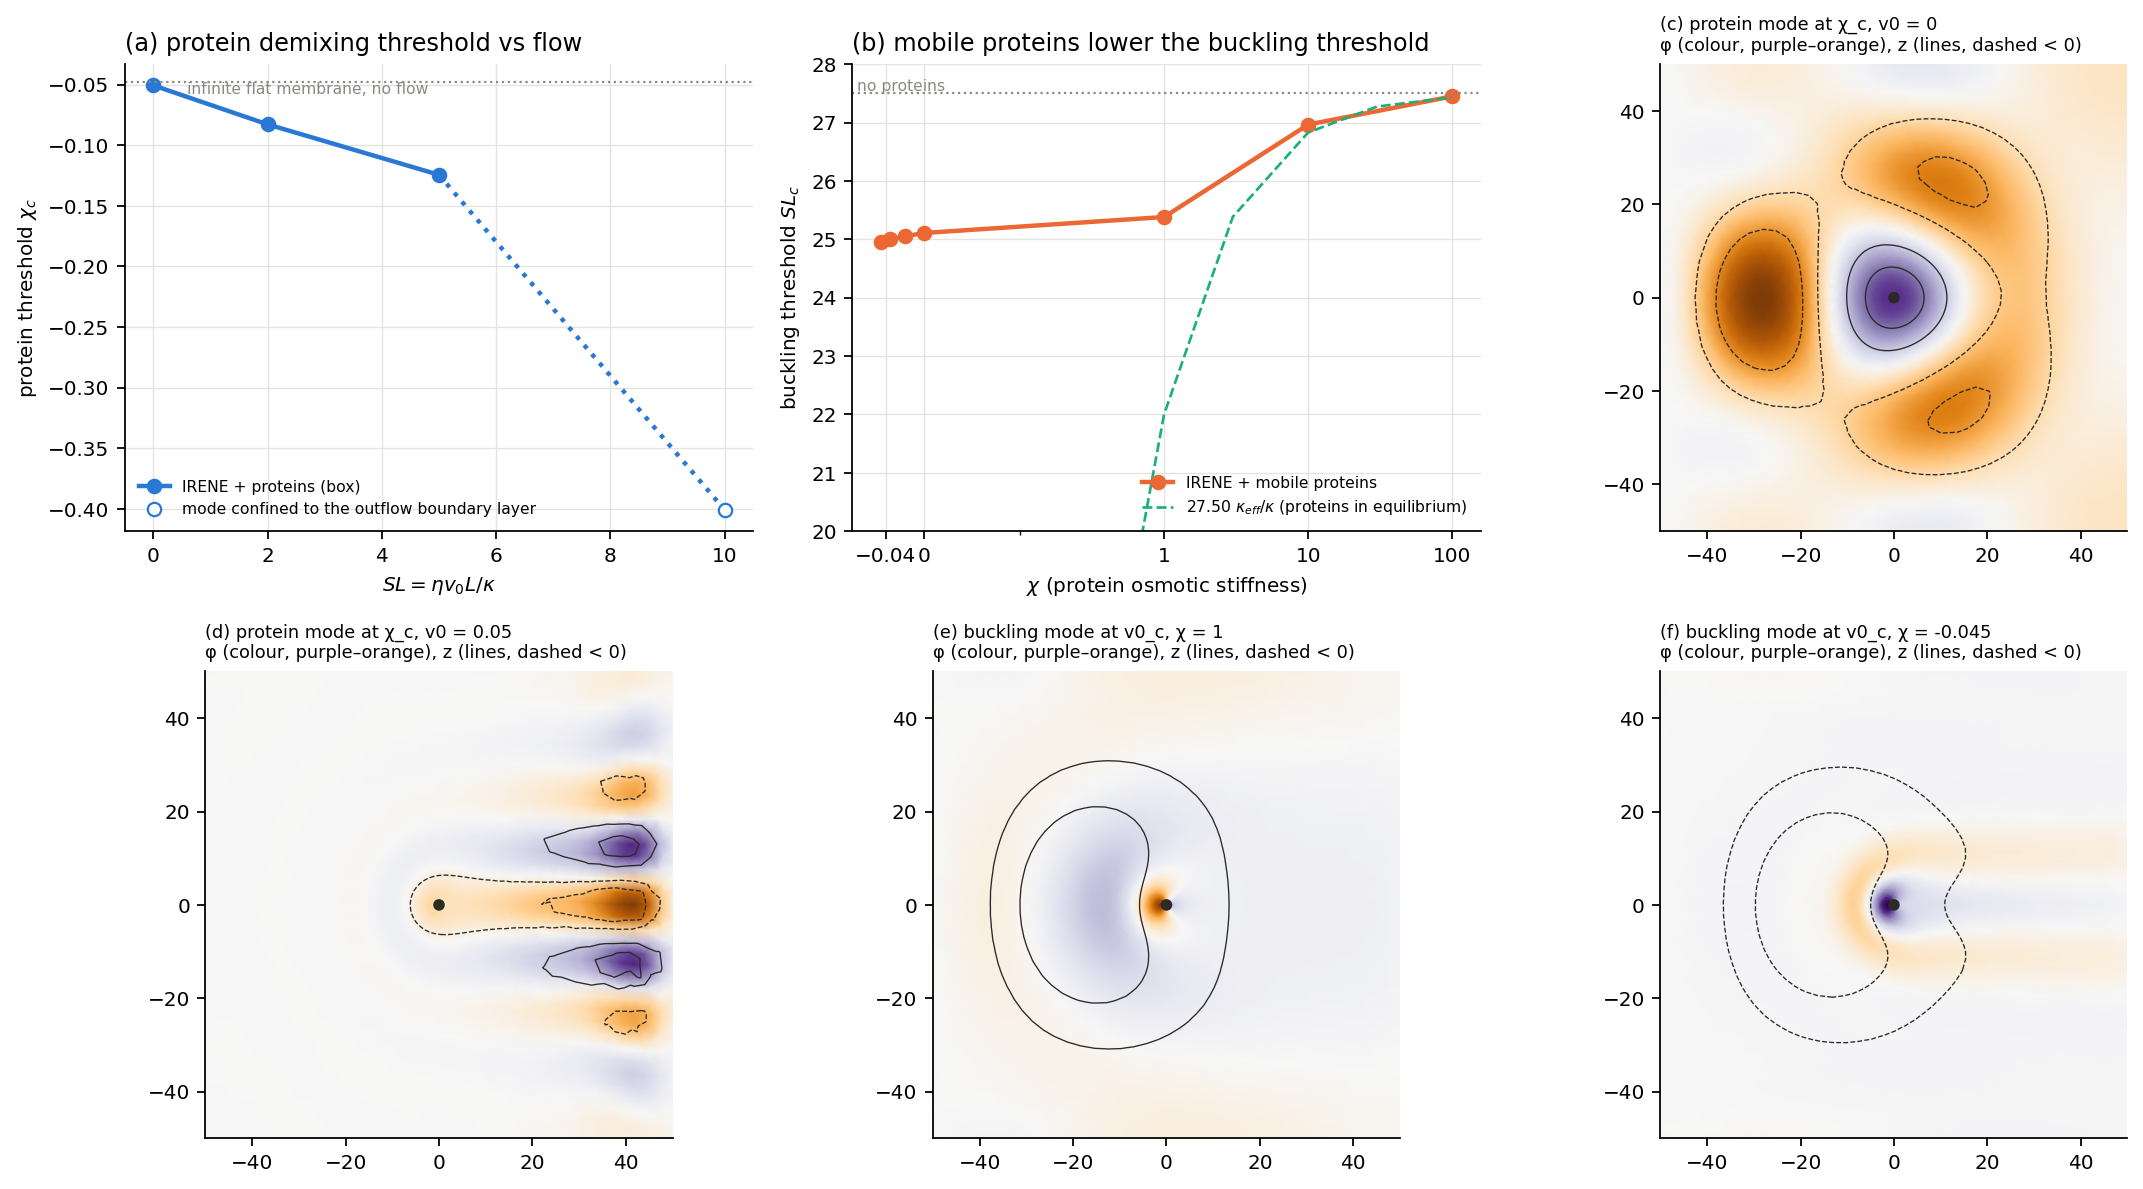
\includegraphics[width=\linewidth,height=182mm,keepaspectratio]{figures/membrane_r4_proteins.png}\captionof{figure}[Archived figure]{Earlier mobile-protein thresholds with no-flux outflow. The high-flow demixing mode is an outflow-layer artifact. The final absorbing-outflow mobility study replaces those high-flow thresholds. \textit{Source:} \path{Ruben/membrane_stability/figures/r4_proteins.png}. First added 2026-10-01.}\end{center}
\clearpage
\begin{center}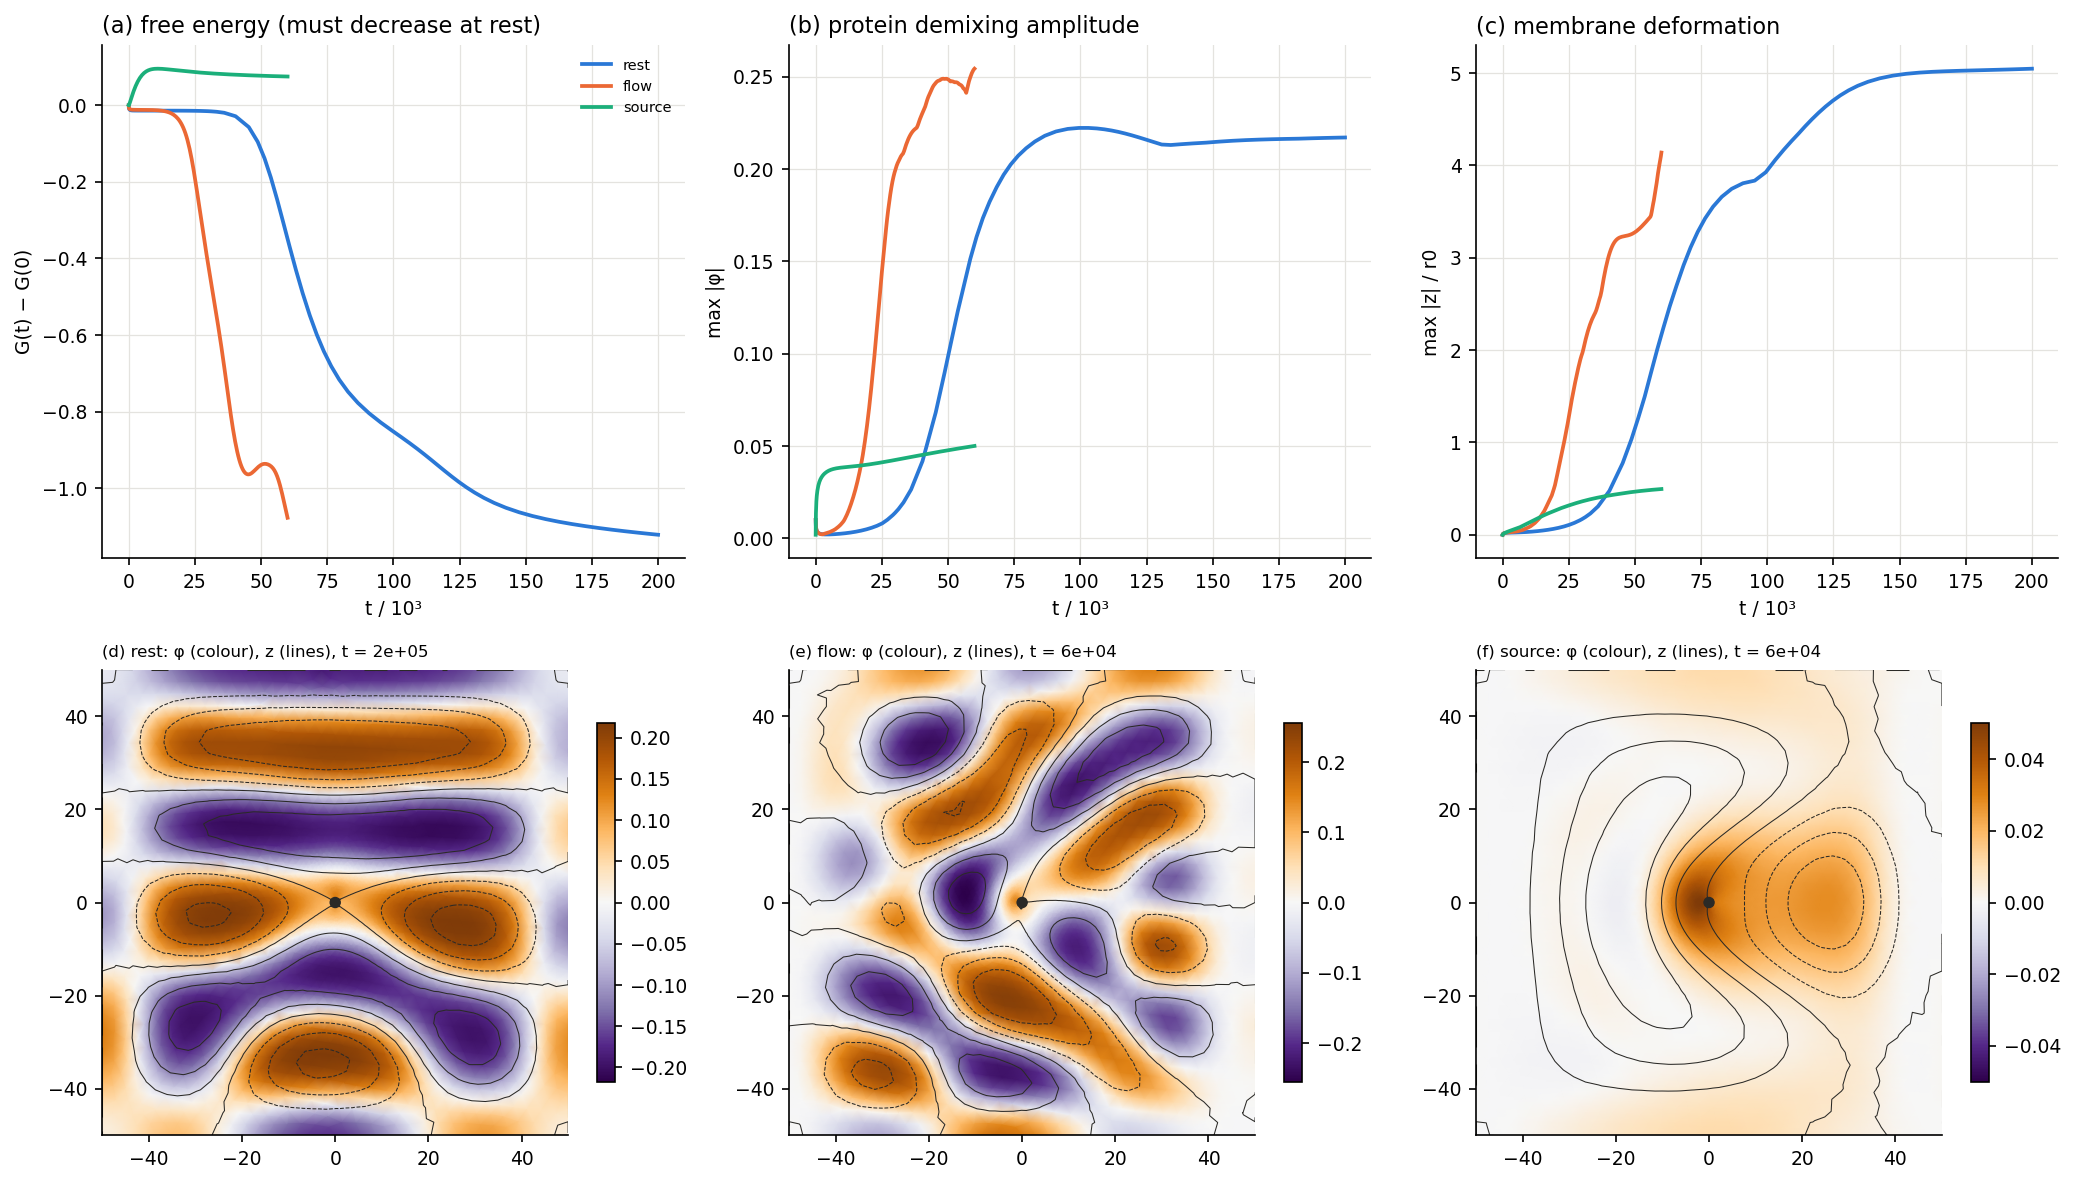
\includegraphics[width=\linewidth,height=182mm,keepaspectratio]{figures/membrane_r5_proteins_dyn.png}\captionof{figure}[Archived figure]{Consistent nonlinear mobile-protein dynamics: no-flow energy relaxation, amplitude saturation, flow-elongated domains, and a source-driven plume. Open reservoirs/sinks mean global protein conservation must include boundary exchange. \textit{Source:} \path{Ruben/membrane_stability/figures/r5_proteins_dyn.png}. First added 2026-10-02.}\end{center}
\clearpage
\begin{center}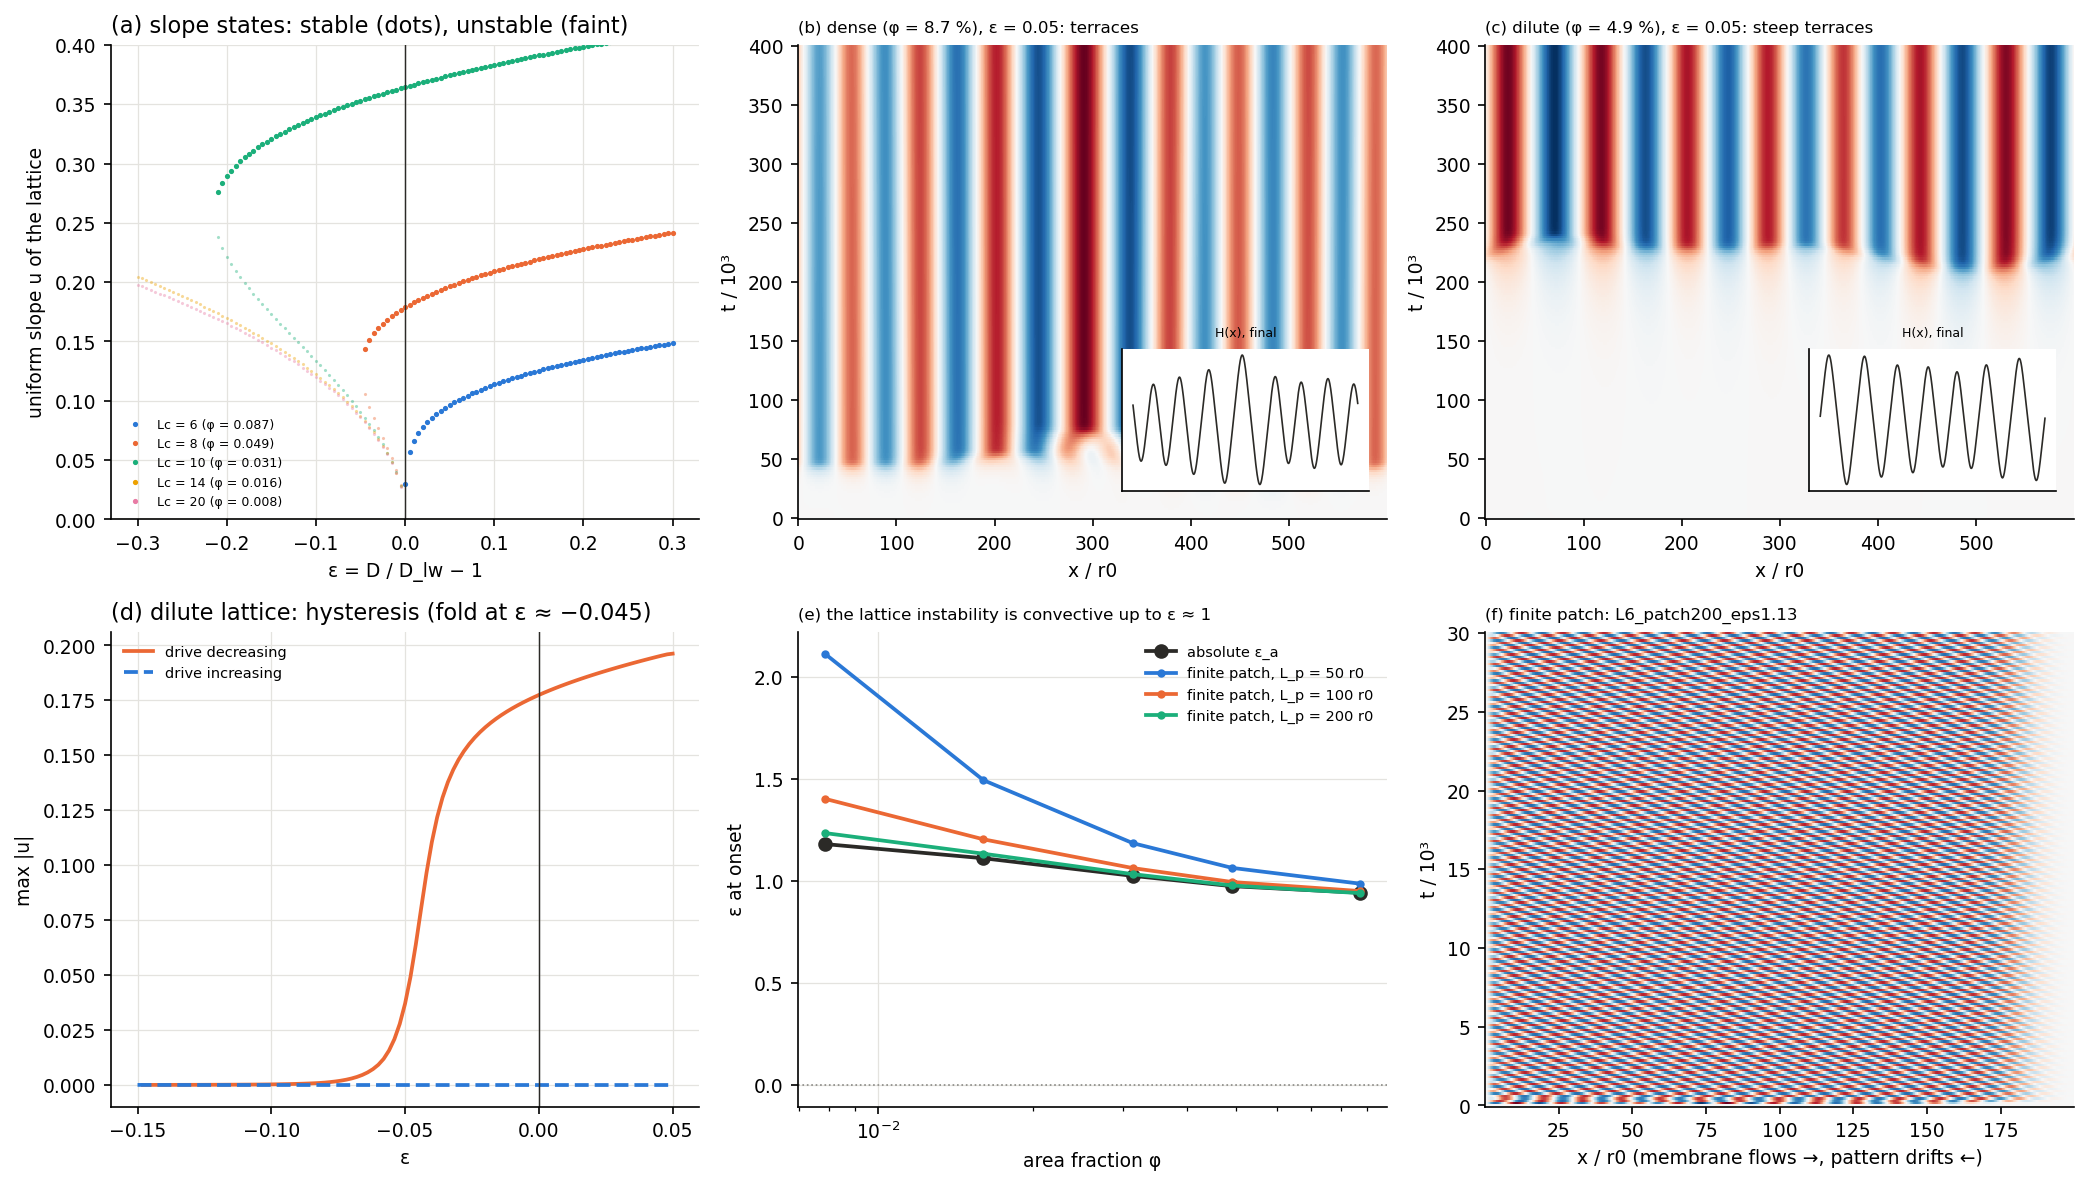
\includegraphics[width=\linewidth,height=182mm,keepaspectratio]{figures/membrane_r5_slope_equation.png}\captionof{figure}[Archived figure]{One-dimensional homogenized lattice dynamics: continuous or hysteretic slope states, coarsening terraces, and finite-patch drift. The absolute-threshold estimate uses a long-wave model near the edge of its spatial validity. \textit{Source:} \path{Ruben/membrane_stability/figures/r5_slope_equation.png}. First added 2026-10-02.}\end{center}
\clearpage
\begin{center}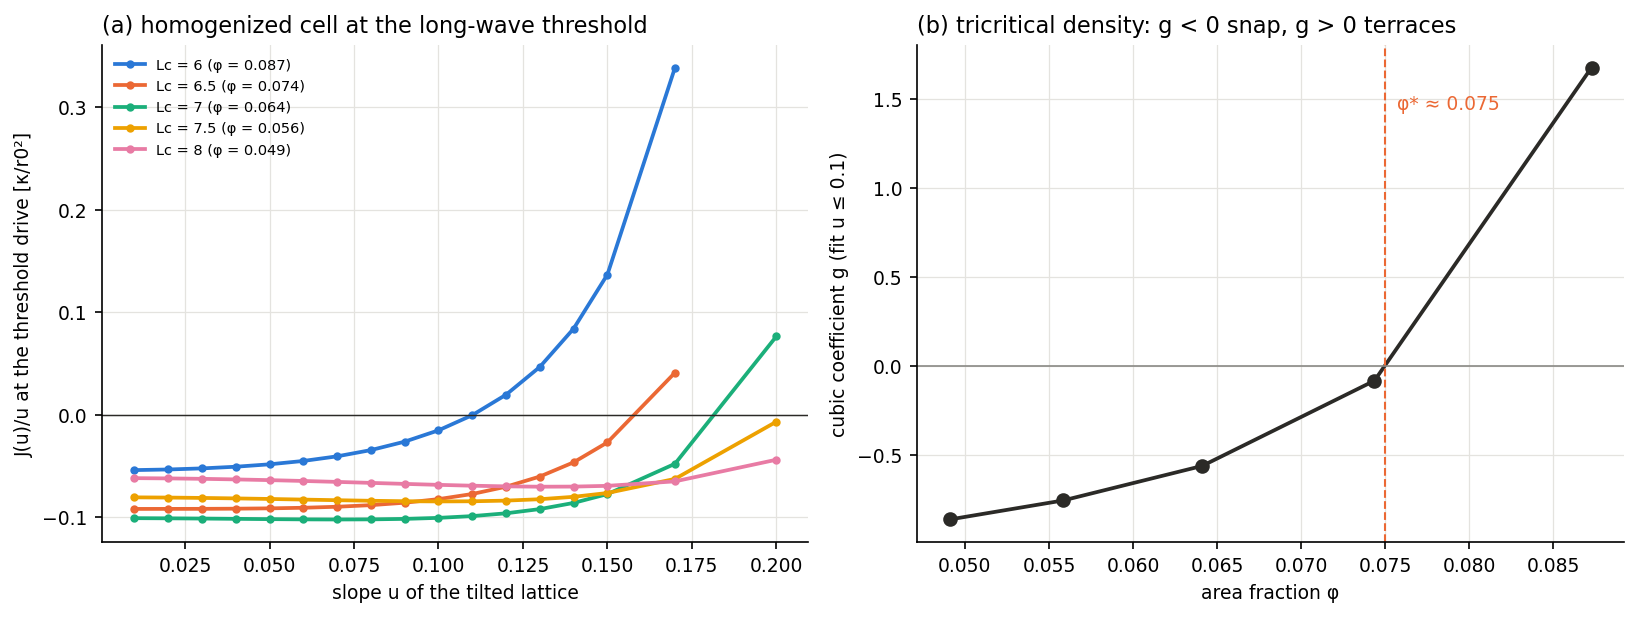
\includegraphics[width=\linewidth,height=86mm,keepaspectratio]{figures/membrane_r5_tricritical.png}\captionof{figure}[Archived figure]{Small-slope nonlinear-cell fits locating the cubic sign change near anchored-disc area fraction 7.5 percent. This onset diagnostic uses a narrower fitting window than the later two-dimensional finite-amplitude polynomial. \textit{Source:} \path{Ruben/membrane_stability/figures/r5_tricritical.png}. First added 2026-10-02.}\end{center}
\begin{center}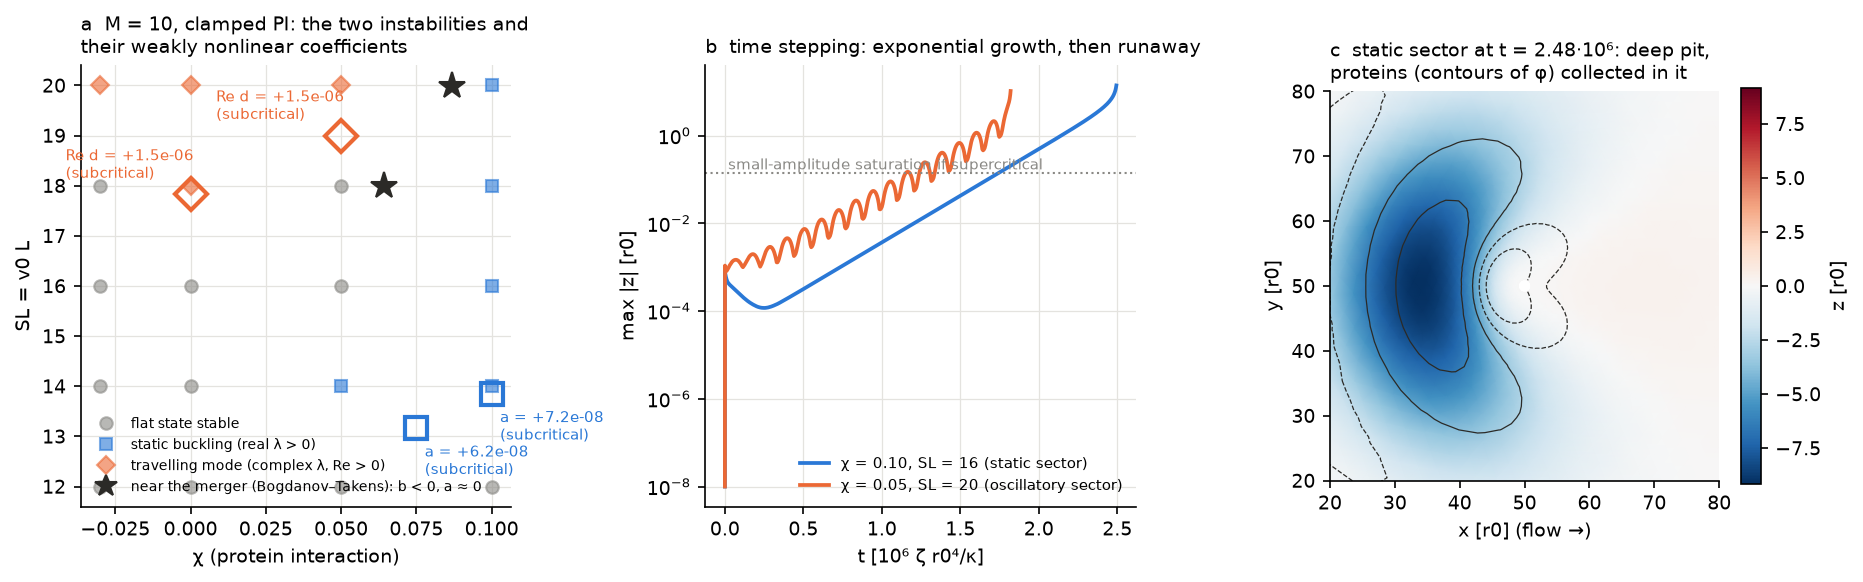
\includegraphics[width=\linewidth,height=86mm,keepaspectratio]{figures/membrane_r6_codim2.png}\captionof{figure}[Archived figure]{Clamped-protein, intermediate-mobility eigenvalue sectors and nonlinear runaway. The nearly vanishing eigenvalues motivate a degenerate Bogdanov-Takens-type interpretation; an exact double-zero location and quintic unfolding remain unresolved. \textit{Source:} \path{Ruben/membrane_stability/figures/r6_codim2.png}. First added 2026-10-03.}\end{center}
\clearpage
\begin{center}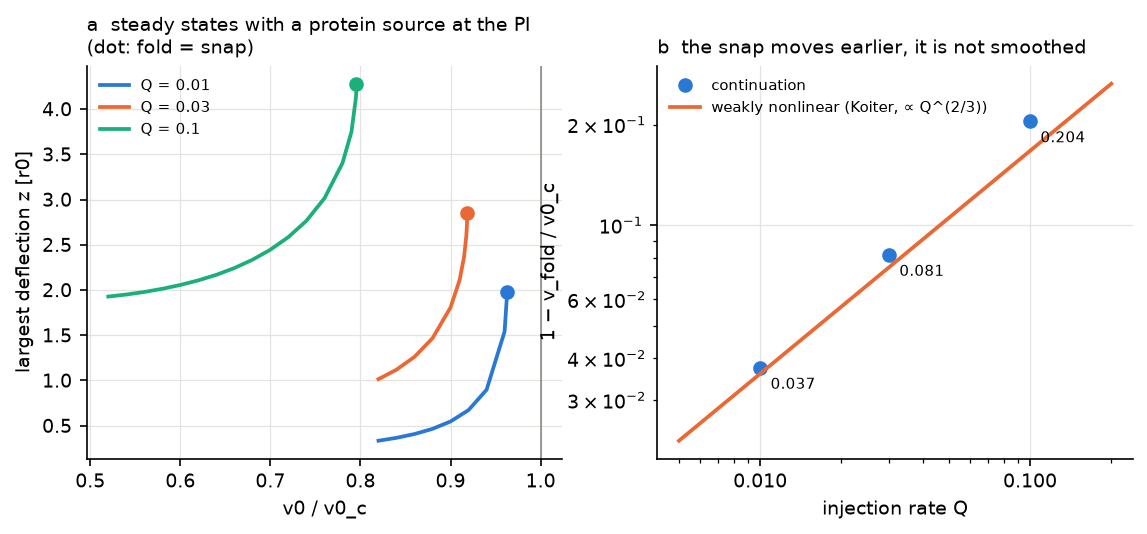
\includegraphics[width=\linewidth,height=86mm,keepaspectratio]{figures/membrane_r6_wake.png}\captionof{figure}[Archived figure]{Source-induced folds and the Koiter prediction. Recruitment is an imperfection that advances rather than removes the snap. The largest-source case is outside the smallest-amplitude cubic regime. \textit{Source:} \path{Ruben/membrane_stability/figures/r6_wake.png}. First added 2026-10-03.}\end{center}
\begin{center}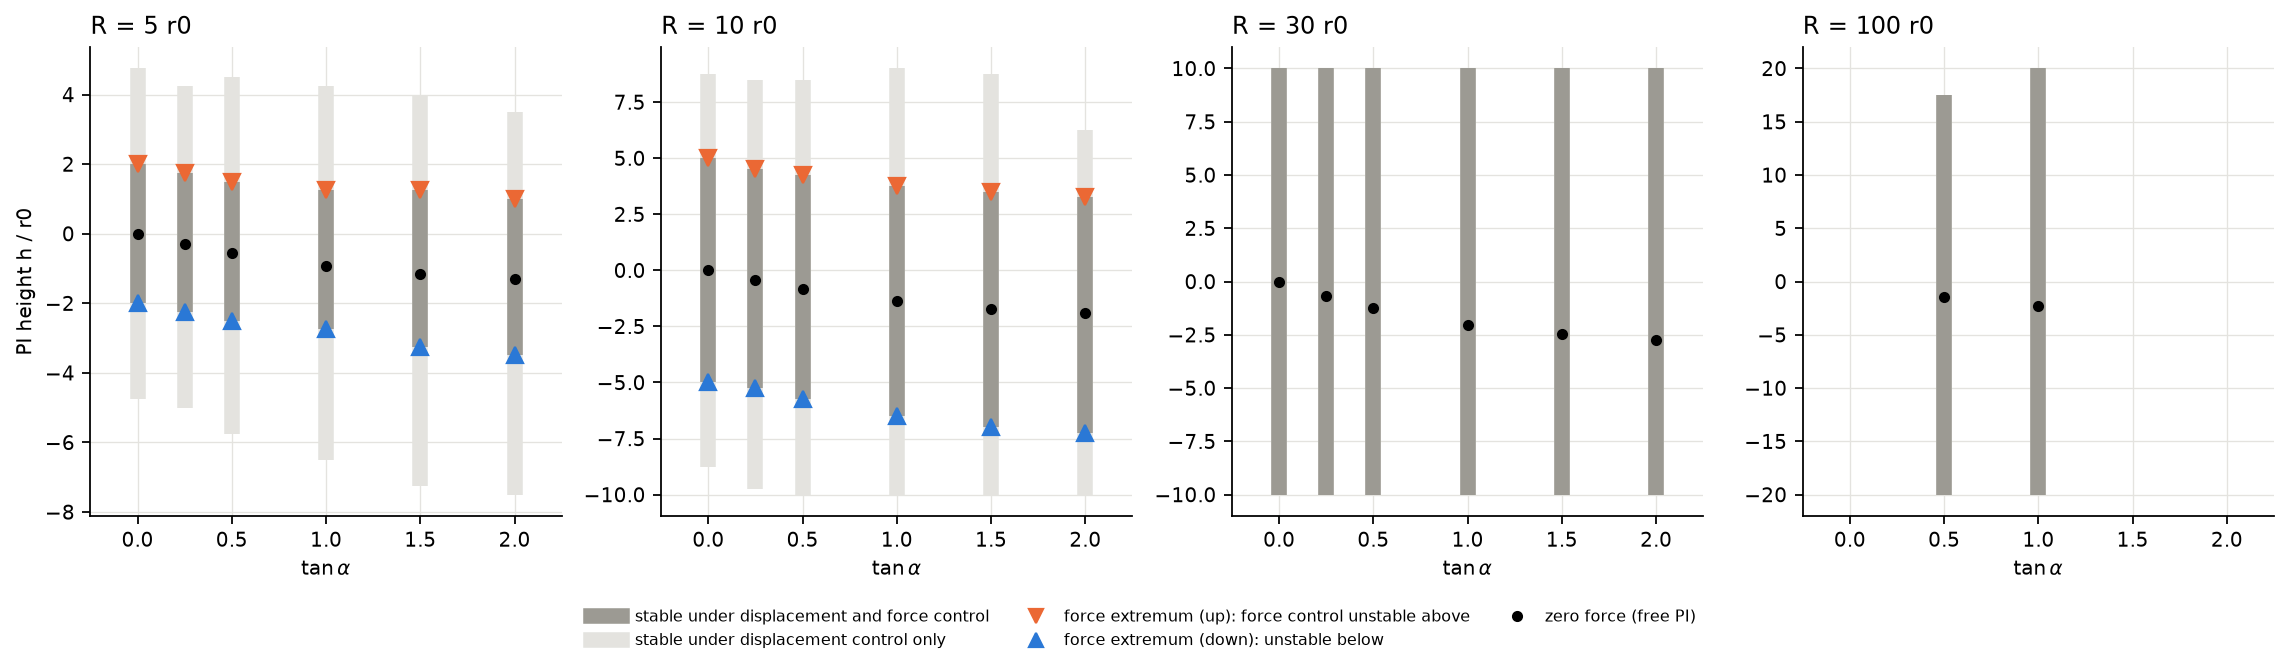
\includegraphics[width=\linewidth,height=86mm,keepaspectratio]{figures/membrane_ring_stability_diagram.png}\captionof{figure}[Archived figure]{Height/contact-slope ring stability diagram over the computed windows. The force-control boundaries are virtual-work force extrema; height-controlled branches remain stable. Grey endpoints indicate limits of the sampled branch. \textit{Source:} \path{Ruben/membrane_stability/figures/ring_stability_diagram.png}. First added 2026-09-30.}\end{center}
\clearpage
\begin{center}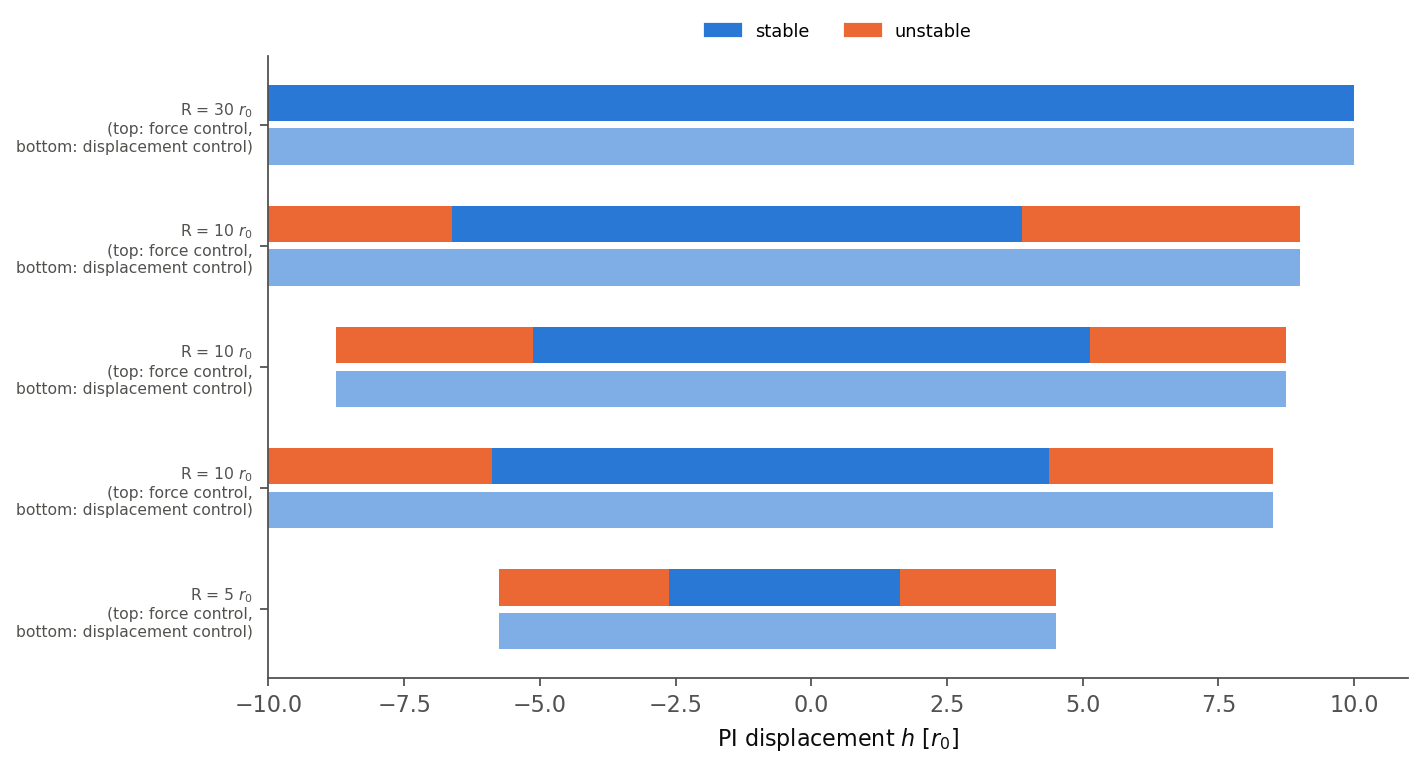
\includegraphics[width=\linewidth,height=182mm,keepaspectratio]{figures/membrane_stability_summary.png}\captionof{figure}[Archived figure]{Ring control-ensemble summary. Force-controlled softening segments are unstable even when the fixed-height shape spectrum remains stable. \textit{Source:} \path{Ruben/membrane_stability/figures/stability_summary.png}. First added 2026-09-29.}\end{center}
\clearpage
\begin{center}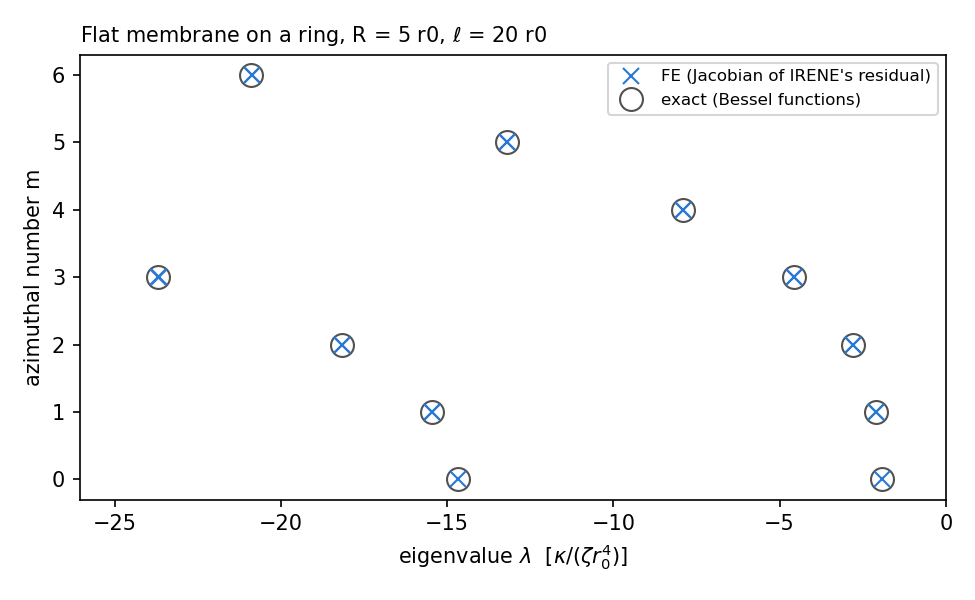
\includegraphics[width=\linewidth,height=182mm,keepaspectratio]{figures/membrane_flat_ring_R5_coarse.png}\captionof{figure}[Archived figure]{Coarse-mesh flat-annulus eigenvalues by azimuthal number compared with the exact Bessel spectrum. This is a separate asset from the fine-mesh check with the same original basename. \textit{Source:} \path{Ruben/membrane_stability/results/checks/flat_ring_R5/check_flat_membrane.png}. First added 2026-09-29.}\end{center}
\clearpage
\begin{center}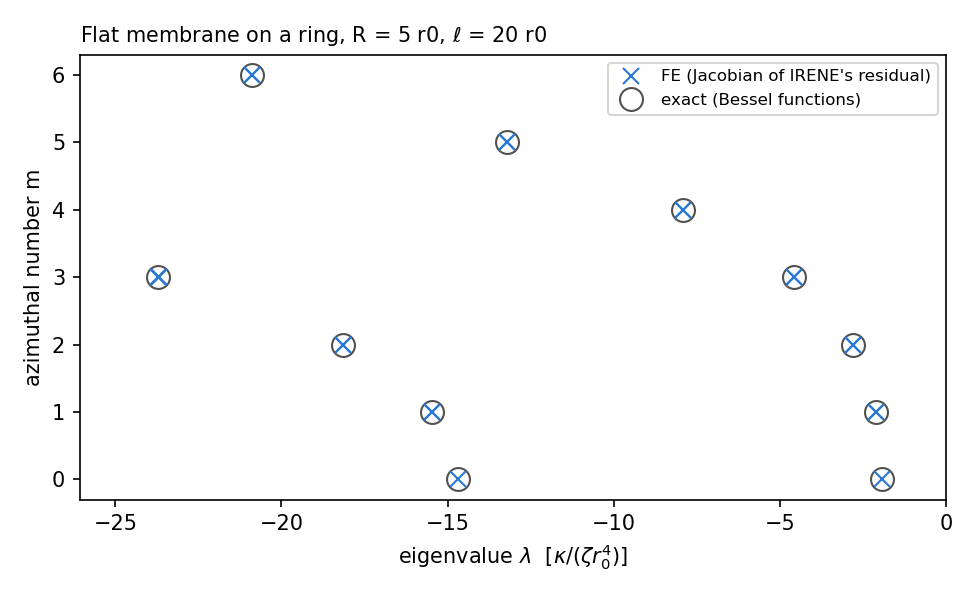
\includegraphics[width=\linewidth,height=182mm,keepaspectratio]{figures/membrane_flat_ring_R5_fine.png}\captionof{figure}[Archived figure]{Fine-mesh flat-annulus spectrum. Refinement reduces the maximum discrepancy to about 2.3 times ten to the minus four across the tested twenty eigenvalues. \textit{Source:} \path{Ruben/membrane_stability/results/checks/flat_ring_R5_fine/check_flat_membrane.png}. First added 2026-09-29.}\end{center}
\clearpage
